\documentclass[a4paper,12pt, oneside]{book}

% \usepackage{fullpage}
\usepackage[italian]{babel}
\usepackage[utf8]{inputenc}
\usepackage{amssymb}
\usepackage{amsthm}
\usepackage{csquotes}
\usepackage{graphics}
\usepackage{amsfonts}
\usepackage{listings}
\usepackage{amsmath}
\usepackage{amstext}
\usepackage{engrec}
\usepackage{rotating}
\usepackage{verbatim}
\usepackage[safe,extra]{tipa}
%\usepackage{showkeys}
\usepackage{multirow}
\usepackage{hyperref}
\usepackage{microtype}
\usepackage{fontspec}
\usepackage{enumerate}
\usepackage{svg}
\usepackage{braket}
\usepackage{physics}
\usepackage{marginnote}
\usepackage{pgfplots}
\usepackage{cancel}
\usepackage{polynom}
\usepackage{booktabs}
\usepackage{enumitem}
\usepackage{framed}
\usepackage{pdfpages}
\usepackage{pgfplots}
\usepackage{algorithm}
% \usepackage{algpseudocode}
\usepackage[cache=false]{minted}
\usepackage{mathtools}
\usepackage[noend]{algpseudocode}
\usepackage{biblatex}
\addbibresource{biblio.bib}
\usepackage{tikz}\usetikzlibrary{er}\tikzset{multi  attribute /.style={attribute
    ,double  distance =1.5pt}}\tikzset{derived  attribute /.style={attribute
    ,dashed}}\tikzset{total /.style={double  distance =1.5pt}}\tikzset{every
  entity /.style={draw=orange , fill=orange!20}}\tikzset{every  attribute
  /.style={draw=MediumPurple1, fill=MediumPurple1!20}}\tikzset{every
  relationship /.style={draw=Chartreuse2,
    fill=Chartreuse2!20}}\newcommand{\key}[1]{\underline{#1}}
  \usetikzlibrary{arrows.meta}
  \usetikzlibrary{decorations.markings}
  \usetikzlibrary{arrows,shapes,backgrounds,petri, trees}
\tikzset{
  place/.style={
        circle,
        thick,
        draw=black,
        minimum size=6mm,
    },
  transition/.style={
    rectangle,
    thick,
    fill=black,
    minimum width=8mm,
    inner ysep=2pt
  },
  transitionv/.style={
    rectangle,
    thick,
    fill=black,
    minimum height=8mm,
    inner xsep=2pt
  }
} 
\usetikzlibrary{automata,positioning}
\usepackage{fancyhdr}
\pagestyle{fancy}
\fancyhead[LE,RO]{\slshape \rightmark}
\fancyhead[LO,RE]{\slshape \leftmark}
\fancyfoot[C]{\thepage}
\definecolor{darkgreen}{rgb}{0.03,0.43, 0.30}
\usepackage[usenames,dvipsnames]{pstricks}
\usepackage{epsfig}
\usepackage{pst-grad} % For gradients
\usepackage{pst-plot} % For axes
\usepackage[space]{grffile} % For spaces in paths
\usepackage{etoolbox} % For spaces in paths
%\usepackage{authblk} % authors
\makeatletter % For spaces in paths
\patchcmd\Gread@eps{\@inputcheck#1 }{\@inputcheck"#1"\relax}{}{}
\makeatother
\title{Appunti di Machine Learning}
\author{UniShare\\\\Davide Cozzi\\\href{https://t.me/dlcgold}{@dlcgold}\\\\and\\\\Mario Avolio\\\href{https://www.marioavolio.ml/}{www.marioavolio.ml}}
\date{}

\pgfplotsset{compat=1.13}
\begin{document}
\begin{titlepage}
    \begin{center}
        \vspace*{1cm}
            
        \Huge
        \textbf{Appunti di Machine Learning}
            
        \vspace{0.5cm}
        \LARGE
        Una risorsa Free e Open Source per Studiare
            
        \vspace{1.5cm}
            
        \textbf{\href{https://t.me/dlcgold}{Davide Cozzi} \\ \href{https://www.marioavolio.ml/}{Mario Avolio}}
            
        \vfill
            
        \vspace{0.8cm}
            
            \begin{figure}[h]
                \centering
                 
\includegraphics[width=0.4\textwidth]{img/studying.png}
            \end{figure}
        \Large
        Dipartimento di Informatica Sistemistica e Comunicazione\\
        Università degli Studi di Milano-Bicocca\\
        Italia\\
    \end{center}
\end{titlepage}

\definecolor{shadecolor}{gray}{0.90}
\setlist{leftmargin = 2cm}
\newcommand{\normm}[1]{\left\lVert#1\right\rVert}
\newtheorem{teorema}{Teorema}
\newtheorem{definizione}{Definizione}
\newtheorem{esempio}{Esempio}
\newtheorem{corollario}{Corollario}
\newtheorem{lemma}{Lemma}
\newtheorem{osservazione}{Osservazione}
\newtheorem{nota}{Nota}
\newtheorem{esercizio}{Esercizio}
\algdef{SE}[DOWHILE]{Do}{doWhile}{\algorithmicdo}[1]{\algorithmicwhile\ #1}



%----------------------------------------------------------------------------------------
%	LIST OF CONTENTS/FIGURES/TABLES PAGES
%----------------------------------------------------------------------------------------

\tableofcontents % Prints the main table of contents

% \listoffigures % Prints the list of figures

\renewcommand{\chaptermark}[1]{%
  \markboth{\chaptername
    \ \thechapter.\ #1}{}}
\renewcommand{\sectionmark}[1]{\markright{\thesection.\ #1}}
\newcommand{\floor}[1]{\lfloor #1 \rfloor}
\newcommand{\MYhref}[3][blue]{\href{#2}{\color{#1}{#3}}}%


% Here is the abstract.
\chapter*{Premessa}
\textbf{Sebbene, questo nobile gesto vuole essere una risorsa free e open source per aiutare gli studenti, è doveroso sottolineare che questo libro non è stato scritto da professori dell'UnimiB ma da studenti. Non è quindi da considerarsi una risorsa ufficiale. Alcuni contenuti di questo testo riprendono slide di alcuni corsi o elementi di alcuni libri. In particolare si trarrà spesso spunto dal libro \textit{Intelligenza artificiale. Un approccio moderno di Libro di Peter Norvig e Stuart J. Russell}~\cite{russell2005intelligenza}. \\ Si vuole menzionare che alcuni appunti sono tratti dal corso di Machine Learning, dell'università di Stanford, del professor \href{https://scholar.google.com/citations?user=mG4imMEAAAAJ&hl=it&oi=ao}{Andrew Ng}. \\ Si ringrazia Freepik di www.flaticon.com per l'icona della prima pagina.}

%---------- INTRODUCTION -----
\chapter{Apprendimento delle Osservazioni}
\label{Capitolo 1}
Questo capitolo tratta dell'\textbf{apprendimento induttivo} che scaturisce dalle osservazioni. In particolare descriveremo come si possono apprendere semplici teorie nella logica proposizionale\footnote{Da Wikipedia: La logica proposizionale è un linguaggio formale con una semplice struttura sintattica, basata fondamentalmente su proposizioni elementari e su connettivi logici di tipo vero-funzionale, che restituiscono il valore di verità di una proposizione in base al valore di verità delle proposizioni connesse.}.
\section{Forme di apprendimento}
Si può pensare a un agente, che è in grado di apprendere, come un insieme di due elementi:
\begin{itemize}
    \item \textbf{elemento esecutivo} che decide quali azioni intraprendere.
    \item \textbf{elemento di apprendimento} che modifica quello esecutivo in modo che prenda decisioni migliori. Esso è influenzato da tre aspetti principali:
    \begin{itemize}
        \item Le \textbf{componenti} che dovranno essere apprese.
        \item Il tipo di \textbf{feedback} disponibile per l'apprendimento di tali componenti.
        \item La \textbf{rappresentazione} utilizzata.
    \end{itemize}
\end{itemize}
\subsection{Tipologia di feedback di un elemento di apprendimento}
Solitamente il \textit{tipo di feedback} disponibile è il fattore più importante per determinare la natura del problema di apprendimento affrontato dall'agente.
\begin{enumerate}
  \item \textbf{Apprendimento supervisionato}: vengono forniti a priori
  esempi di comportamento e si suppone che il \textit{trainer} dia la risposta
  corretta per ogni input, mentre il learner usa gli esempi forniti per
  apprendere. L'esperienza è fornita da un insieme di coppie di valori raffiguranti il \textit{Training Set}:
  \[S\equiv\{(x_1, y_1),(x_2, y_2),\ldots,(x_n, y_n)\}\]
  Per ogni input ipotetico $x_i$ il trainer restituisce il corretto
  $y_i$
  \item \textbf{Apprendimento non supervisionato}: si tentano di riconoscere degli
  \textit{schemi} nell'input senza che vengano fornite indicazioni sui valori in uscita. Non c'è
  target e si ha \textit{libertà di classificazione}. Si cerca una
  \textit{regolarità} e una \textit{struttura} insita nei dati. In questo caso
  si ha: 
  \[S\equiv\{x_1, x_2,\ldots, x_n\}\]
  Il clustering è un tipico problema di apprendimento non supervisionato. Non si
  ha spesso un metodo oggettivo per stabilire la qualità delle prestazioni che vengono quindi
  valutate da umani
  \item \textbf{Apprendimento per rinforzo}: bisogna apprendere tramite il
  \textit{learner} sulla base della risposta dell’ambiente alle proprie azioni. Si lavora con
  un \textit{addestramento continuo}, aggiornando ripetutamente le ipotesi con l'arrivo di
  nuovi dati (ad esempio per una macchina che deve giocare a un gioco). Durante la
  fase di test bisogna conoscere le prestazioni e valutare la correttezza di
  quanto appreso. Il learner viene addestrato tramite \textit{rewards} e quindi
  apprende una strategia per massimizzarle, detta
  \textbf{strategia di comportamento}.Per valutare la prestazione si cerca di
  massimizzare ``a lungo termine'' la ricompensa complessivamente ottenuta.
\end{enumerate}
%----------------------------------------------------------------------------------------
%	SECTION 
%----------------------------------------------------------------------------------------
\section{Apprendimento induttivo}
Un algoritmo per l'apprendimento deterministico supervisionato riceve in ingresso il valore di una funzione sconosciuta in alcuni punti e deve cercare di ricostruirla nel modo più fedele possibile. Più formalmente, diciamo che un \textbf{esempio} è una coppia $(x, f(x))$, in cui $x$ è l'input e $f(x)$ è l'output della funzione applicata all'input. Il compito dell'\textbf{induzione} (inferenza induttiva pura) è:\\
\textit{data una collezione di esempi di $f$, restituire una funzione $h$ che approssima $f$.}\\
Tale funzione $h$ prende il nome di \textbf{ipotesi} e la vedremo nei capitoli successivi. Il problema fondamentale risiede nel cercare di \textbf{generalizzare} bene tale funzione, ovvero trovare una $h$ che potrà predire correttamente esempi che \textbf{non ha ancora incontrato}. 
\newpage
\begin{shaded}
  \begin{itemize}
  
    \item $x\in X$, \textbf{istanza}: un singolo ``oggetto'' preso dallo
    \textbf{spazio delle istanze}. Ogni \textbf{istanza} è rappresentata tramite
    un \textbf{vettore di attributi unici} (un attributo per posizione del
    vettore). In termini probabilistici questo equivale a un \textit{evento elementare}.
    
    \item $X$, \textbf{spazio delle istanze}: ovvero la collezione di tutte le
    possibili istanze utili per qualche compito di \textit{learning}. 
    In termini statistici lo \textit{spazio delle istanze} non è altro che lo 
    \textbf{spazio campionario} \footnote{Insieme di tutti i possibili eventi elementari.}
    
    \item $c$, \textbf{concetto}, $c\subseteq X$: ovvero un sottoinsieme dello \textit{spazio delle istanze} che descrive una \textit{classe} d'istanze alla quale siamo interessati per costruire un modello di \textit{machine learning}. In pratica raccolgo quel sottoinsieme d'istanze che mi garantiscono, per esempio, uno o più attributi validi al mio modello. La nozione statistica equivalente è quella di \textit{evento} (ovvero un sottoinsieme dello \textit{spazio campione}).\\ 
    Si ha quindi che, preso un concetto $A\subseteq X$:
    \[f_A:X\to\{0, 1\}\]
    
    Si ottiene: 
    
    \[f_a(x)=
      \begin{cases}
        1& \mbox{se } x\in A\\
        0& \mbox{altrimenti}
      \end{cases}
    \]
    
    \item $(x, f(x))$, \textbf{esempio}: Ovvero un'istanza etichettata con la sua classe di appartenenza. La funzione $f$ è detta \textbf{funzione target}.
    
    \item $D=\{(x_1, f(x_1)),\ldots,(x_n, f(x_n))\}$, \textbf{Training Set}:
    ovvero è la raccolta degli esempi. Qualora si avesse a che fare con un \textit{training non supervisionato} si avrebbe:
    $D=\{x_1,\ldots, x_n\}$
    
    \item \textbf{Ipotesi (o Modello)}, $h\subseteq X$: Essa rappresenta una possibile soluzione al problema. Normalmente simboleggiata da un vettore booleano dove ogni elemento di esso si riferisce a un attributo.
    \begin{itemize}
        \item \textbf{Ipotesi h}: ovvero una congiunzione di vincoli sugli
    attributi. Tale ipotesi è \textbf{consistente}, ovvero è coerente con tutti gli esempi.
    \item \textbf{soddisfazione di un'ipotesi}: un'istanza $x$ soddisfa
    un'ipotesi $h$ sse tutti i vincoli espressi da $h$ sono soddisfatti dai
    valori di $x$ e si indica con:
    \[h(x)=1\]
    \begin{esempio}
      Avendo:
      \[x=\langle S, W, N, S, W, S\rangle \mbox{\textnormal{e}
        }h=\langle S,?,?, S,?, S\rangle\]
      posso dire che $x$ soddisfa $h$.\\
      se invece ho che:
      \[h=\langle S,?,?,\emptyset,?, S\rangle\]
      posso dire che $x$ non soddisfa $h$.
    \end{esempio} 
    \end{itemize}
    
    \item $H$, \textbf{spazio delle ipotesi (spazio dei Modelli)}: insieme d'ipotesi.
    
    
    \item $\{(x_1', f(x_1')),\ldots,(x_n', f(x_n'))\}$, \textbf{test}
    
    
    \item un \textbf{Modello di machine learning} è
    quindi l'\textit{ipotesi migliore}. Questo \textbf{modello predittivo} viene
    addestrato tramite il \textit{training set} e servirà per inferire nuove
    informazioni mai state osservate nel \textit{training set}. 
    
    
    \item \textbf{Linguaggio delle ipotesi}: è il linguaggio che definisce lo
    \textit{spazio delle ipotesi / modelli}
    \begin{esempio}
      Prendiamo un problema semplice di \textit{regressione lineare}.\\
      In questo contesto un'istanza è un punto $(x, y)$, lo spazio delle ipotesi
      è quello formato dalle rette $y=a+bx$ (dove $a$ è il nostro
      \textbf{bias}). Tra tutte queste rette cerco quella che sarà il
      \textbf{modello predittivo}, tramite la quale poter prevedere l'andamento
      dei vari punti (di modo che dato un $x$ sia in grado di stabilire un buon
      $y$)
    \end{esempio}
    
    \item \textbf{Cross validation}: ovvero ripeto $m$ volte la validazione su
    campioni diversi d'input per evitare che un certo risultato derivi dalla
    fortuna. 
  \end{itemize}
\end{shaded}


Il tipo di dato che studieremo comunemente sarà il \textbf{vettore booleano} e la risposta sarà anch'essa di tipo booleano. In questo contesto l'ipotesi è una \textbf{congiunzione di variabili}.\\
Il Machine learning si occupa di trovare, all'interno dello spazio dei modelli, l'ipotesi migliore mediante strategie che si basano sull'analisi del Training Set.
%------------------
Quindi un \textbf{sistema di apprendimento automatico} ricava da un insieme di dati
una conoscenza non fornita a priori al fine di creare dei modelli in grado di \textit{soddisfarli}. 
L'idea è quella di creare un modello in grado di approssimare il più possibile i dati proposti 
in modo tale da trovare una correlazione tra essi. In
quest'ottica bisogna mediare tra \textbf{fit} e \textbf{complessità}. Ogni
sistema dovrà cercare di mediare tra questi due aspetti, dove un \textit{fit}
migliore comporta alta \textit{complessità}. Si ha sempre il rischio di \textbf{overfitting} 
\footnote{In statistica e in informatica, si parla di overfitting (in italiano: adattamento eccessivo, sovradattamento) quando un modello statistico molto complesso si adatta ai dati osservati (il campione) perché ha un numero eccessivo di parametri rispetto al numero di osservazioni.
Un modello assurdo e sbagliato può adattarsi perfettamente se è abbastanza complesso rispetto alla quantità di dati disponibili.
Si sostiene che l'overfitting sia una violazione del principio del rasoio di Occam.}, ovvero:
\begin{itemize}
    \item occorre accettare un inevitabile compromesso tra la complessità dell'ipotesi e il grado di corrispondenza con i dati.
    \item è necessario accettare un compromesso tra l'espressività dello spazio delle ipotesi e la complessità della ricerca d'ipotesi semplici e consistenti all'interno di tale spazio.
\end{itemize}
Definiamo alcuni concetti base:
\begin{itemize}
  \item \textbf{Task (\textit{T})}: il compito da apprendere. È più facile
  apprendere attraverso esempi che codificare conoscenza o definire alcuni
  compiti. Il comportamento della macchina in un ambiente può essere
  diverso da quello desiderato a causa della mutabilità di quest'ultimo, ed è più
  semplice cambiare gli esempi piuttosto che ridisegnare un intero sistema. 
  \item \textbf{Performance (\textit{P})}: la misura della bontà
  dell'apprendimento.
  \item \textbf{Experience (\textit{E})}: l'esperienza sui cui basare
  l'apprendimento. Il tipo di esperienza scelto può variare di molto il risultato e
  il suo successo.
\end{itemize}
In merito alle parti ``software'' distinguiamo:
\begin{itemize}
  \item \textbf{Learner}: la parte di programma che impara dagli esempi in modo
  automatico.
  \item \textbf{Trainer}: il \textit{dataset (o Training Set)} che fornisce esperienza al
  \textit{learner}.
\end{itemize}
Durante l'\textbf{apprendimento} si analizzano gli esempi dati in ingresso al fine di generare un modello che li soddisfi.\\
Approfondiamo il discorso relativo all'\textit{esperienza}. Innanzitutto nel
momento della scelta bisogna valutare la rappresentatività dell'esperienza. 
Oltre ad apprendere, il \textit{learner} ha la facoltà di controllare e manipolare la propria esperienza:
\begin{itemize}
  \item L'esperienza può essere fornita al learner senza che esso possa
  interagire.
  \item Il learner può porre domande su quegli esempi che non risultano chiari. 
\end{itemize}
\textbf{L'esperienza DEVE essere presentata in modo causale.}\\
Esistono due tipi di esperienza:
\begin{enumerate}
  \item \textbf{Diretta}: dove il learner può acquisire informazioni utili
  direttamente dagli esempi o dover inferire indirettamente da essi
  l’informazione necessaria.
  \item \textbf{Indiretta}
\end{enumerate}
Possiamo inoltre distinguere due tipi di apprendimento rispetto al \textbf{learner}:
\begin{enumerate}
  \item \textbf{Attivo}: il \textit{learner} può fare ``domande'' sui dati
  a sua disposizione. 
  \item \textbf{Passivo}: il \textit{learner} apprende solo a partire dai
  dati disponibili. 
\end{enumerate}

%1

%---------- Concept Learning -----
\chapter{Concept Learning}
\label{Capitolo 2}
%%%%
In questo capitolo studieremo metodi di apprendimento che possono mettere a frutto la \textbf{conoscenza a priori}. In particolare essa verrà rappresentata come un insieme di teorie generali di \href{https://it.wikipedia.org/wiki/Linguaggio_del_primo_ordine}{logica del primo ordine\footnote{Da Wikipedia: Nella logica matematica il linguaggio del primo ordine è un linguaggio formale che serve per gestire meccanicamente enunciati e ragionamenti che coinvolgono i connettivi logici, le relazioni e i quantificatori "per ogni ..." (∀) ed "esiste..." (∃). L'espressione "del primo ordine" indica che c'è un insieme di riferimento e i quantificatori possano riguardare solo gli elementi di tale insieme e non i sottoinsiemi; ad esempio si può dire "per tutti gli x elementi dell'insieme vale P(x)" ma non si può dire "per tutti i sottoinsiemi A vale P(A)" (le teorie in cui ci sono quantificatori che spaziano sui sottoinsiemi dell'insieme di riferimento sono dette invece del secondo ordine).}}.
\section{Una formulazione logica dell'apprendimento}
Nel capitolo precedente abbiamo definito l'apprendimento induttivo puro come il processo mediante il quale si cerca un'ipotesi che concorda con gli esempi osservati. Ora specializzeremo tale definizione per il caso in cui l'ipotesi sia rappresentata da un insieme di formule logiche. Questo approccio consente di creare delle ipotesi in maniera incrementale; inoltre consente di sfruttare la conoscenza pregressa, perché le formule già note possono aiutare la classificazione di nuovi esempi. Il \textbf{concept learning} è la ricerca, nello spazio delle ipotesi, di funzioni che assumano valori all'interno di $\{0, 1\}$. In altre parole si parla di funzioni che hanno come dominio lo \textbf{spazio delle ipotesi} e come codominio $\{0, 1\}$:
\[f:H\to\{0, 1\}\]
Volendo si possono usare insiemi e non funzioni.\\
\subsection{Esempi e Ipotesi}
Un esempio è un oggetto descritto da una formula logica e gli attributi sono predicati unari. L'intero insieme di addestramento sarà quindi espresso da una congiunzione di tutte le descrizioni e delle formule di classificazione. Lo scopo dell'apprendimento induttivo in ambito logico è trovare un'espressione equivalente al \textbf{predicato obiettivo} (la nostra ipotesi) utilizzabile per classificare correttamente gli esempi.
Si cerca quindi con opportune procedure la miglior ipotesi che si adatta
meglio al concetto implicato dal \textit{training set}.
In questo contesto si cerca di capire quale funzione booleana è adatta al mio addestramento. In altre parole si cerca di apprendere un'ipotesi booleana partendo da esempi di training composti da input e output (etichetta target + label) della funzione. \\
Nel concept learning un'ipotesi è un insieme di valori di attributi e ogni valore può essere:
\begin{itemize}
  \item Specificata
  \item Non importante: che si indica con ``?'', e che può assumere qualsiasi
  valore. Avere un'ipotesi con tutti i valori del vettore pari a ``?'' implica
  avere l'ipotesi più generale, avendo classificato tutte le istanze solo come
  esempi positivi. 
  \item Nulla: si indica con $\emptyset$. Avere un'ipotesi con tutti i valori
  del vettore pari a $\emptyset$ implica avere l'ipotesi più specifica, avendo
  classificato tutte le istanze solo come esempi negativi. 
\end{itemize}
\begin{esempio}
  Vediamo quindi la rappresentazione di una ipotesi (ipotizzando di avere a che
  fare con solo 4 attributi $A_i$, sempre in prospettiva booleana):
  \[h=\langle 0, 1, ?, 1\rangle = \langle A_1=0, A_2=1, A_3=\,?, A_4=1\rangle\]
  nella realtà, grazie al ``?'' riferito all'istanza, l'ipotesi $h$ è un insieme
  di due ipotesi: 
  \[h\in\{(0, 1, 0, 1),\,(0, 1, 1, 1)\}\]
  passando quindi da una notazione per ipotesi a una insiemistica.\\
  Ricordiamo inoltre che lo spazio delle istanze $X$, dal punto di vista
  insiemistico è:
  \[X=\{(x_1, x_2, x_3, x_3): \,\, x_1\in A_1, x_2\in A_2, x_3\in A_3, x_4\in A_4\}\]
\end{esempio}
\subsubsection{Soddisfacimento e Consistenza}
Ogni ipotesi predice che un certo insieme di esempi e, precisamente quelli che la soddisfano, saranno anche esempi del \textbf{predicato obiettivo}. Questo insieme è chiamato \textbf{estensione del predicato}. \begin{definizione}
  Due ipotesi con estensioni differenti sono quindi logicamente inconsistenti l'una con l'altra, perché le loro previsioni sono discorsi su almeno un esempio.
\end{definizione}
Sia \textit{c(x)} una \textbf{funzione target}, ovvero la funzione che, all'interno di un certo \textit{training set} $D$, esprime il valore di verità di un'istanza.
\begin{definizione}
Si dice che un'istanza $x$ \textbf{soddisfa} i vincoli di $h$ sse $h$ classifica $x$ come
esempio positivo:
\[h(x)=1\]  
Ciò è \textbf{indipendente} dal valore della funzione target associato ad x.
\end{definizione}

\begin{definizione}
 Si dice \textbf{consistente} un'ipotesi $h\in H$ nei confronti di un determinato insieme addestramento sse essa dev'essere consistente con ogni esempio di tale insieme. Ovvero: 
\[h(x)=c(x),\,\forall x\in D\]  
\end{definizione}

Si evince la teoria delle \textbf{ipotesi di apprendimento induttivo} che dice che se la mia $h$ approssima bene nel \textit{training set} allora approssima bene su tutti gli esempi non ancora osservati.\\
Il concept learning è quindi una ricerca del \textit{fit} migliore.
\subsubsection{Falso negativo e Falso positivo}
Se un esempio è un falso positivo o un falso negativo per un'ipotesi, l'esempio e l'ipotesi sono logicamente inconsistenti. Presumendo che l'esempio rappresenti l'osservazione corretta di un fatto, l'ipotesi può quindi essere scartata. Possiamo quindi caratterizzare l'apprendimento induttivo in ambito logico come un processo di \textbf{eliminazione graduale} delle ipotesi che si rivelano inconsistenti con gli esempi.
\begin{itemize}
    \item Un esempio può essere un \textbf{falso negativo} per l'ipotesi se essa predice che dovrebbe essere negativo ma, in effetti, è positivo. L'ipotesi e l'esempio sono quindi logicamente inconsistenti.
    \item Un esempio può essere un \textbf{falso positivo} per l'ipotesi se essa dice che dovrebbe essere positivo ma, in effetti, è negativo.
\end{itemize}
%----------------------------------------------------------------------------------------
%	SECTION 
%----------------------------------------------------------------------------------------
\section{Generalità delle ipotesi}
\begin{definizione}
  Date $h_j, h_k\in H$ booleane e definite su $X$. Si ha che $h_j$ è \textbf{più
    generale o uguale a} $h_k$ (e si scrive con $h_j\geq h_k$) sse:
  \[(h_k(x)=1)\longrightarrow (h_j(x)=1),\,\,\forall x\in X\]
  \textbf{Si impone quindi un ordine parziale}.\\
  Si ha che $h_j$ è \textbf{più generale di} $h_k$ (e si scrive con $h_j> h_k$)
  sse:
  \[(h_j\geq h_k)\land (h_k\not\geq h_j)\]
  Riscrivendo dal punto di vista insiemistico si ha che $h_j$ è \textbf{più
    generale o uguale a} $h_k$ sse:
  \[h_j\supseteq h_k\]
  e che è \textbf{più generale di} $h_k$ sse:
  \[h_j\supset h_k\]
  Dal punto di vista logico si ha che $h_j$ è \textbf{più generale di} $h_k$ sse
  impone meno vincoli di $h_k$ \ref{fig:eulero}
\end{definizione}
\begin{esempio}
  Facciamo un esempio ``giocattolo'' di situazione di \textbf{concept
    learning}.\\ 
  La \textbf{funzione target} (o target concept), ovvero la domanda che ci si pone, è:\\
  \begin{center}
    \textit{In quali tipologie di giorni $A$ apprezza fare sport acquatici?}
  \end{center}
  Abbiamo quindi una serie di attributi per il meteo con i vari valori che
  possono assumere:
  \begin{table}[H]
    \centering
    \begin{tabular}[H]{|c|c|}
      \hline
      \textbf{Attributo} & \textbf{\textit{Possibili valori}}\\
      \hline
      sky & \textit{Sunny, Cloudy, Rainy}\\
      temp & \textit{Warm, Cold}\\
      humid & \textit{Normal, High}\\
      wind & \textit{Strong, Weak}\\
      water & \textit{Warm, Cold}\\
      forecast & \textit{Same, Change}\\
      \hline
    \end{tabular}
  \end{table}
  In ottica \textit{concept learning} si cerca quindi la \textbf{funzione
    target} $enjoySport$ (che sarebbe la nostra funzione $c$): 
  \[enjoySport:X\to\{0, 1\}\]
  Vediamo quindi anche un esempio di \textit{training set} $D$ (per praticità i
  valori degli attributi sono indicati con la sola iniziale):
  \begin{table}[H]
    \centering
    \begin{tabular}[H]{|c|c|c|c|c|c|c|}
      \hline
      \textbf{sky} & \textbf{temp} & \textbf{humid} & \textbf{wind} &         
      \textbf{water} & \textbf{forecast} & \textbf{enjoySport}\\
      \hline
      S & W & N & S & W & S & \color{darkgreen} yes\\
      S & W & H & S & W & S & \color{darkgreen} yes\\
      R & C & H & S & W & C & \color{red} no\\
      S & W & H & S & C & C & \color{darkgreen} yes\\
      \hline
    \end{tabular}
  \end{table}
  Dove nella colonna finale si ha la risposta booleana al problema, è infatti
  l'\textbf{etichetta target} (valore della funzione target per un determinato attributo).\\
  Bisogna quindi cercare un'ipotesi $h$ tale che $h(x)=c(x)$,
  per tutte le istanze nel \textit{training set}.\\
  Un'ipotesi $h$, anch'essa rappresentata come vettore, sarà quindi una
  congiunzione $\land$ di vincoli di valore sugli attributi.
  \label{es:tab}
\end{esempio}
\begin{esempio}
  Vediamo un esempio anche relativo alle nozioni di \textbf{più generale di}.\\
  Si hanno due ipotesi:
  \[h_J=\langle S,?,?,?,?,?\rangle\]
  \[h_k=\langle S,?,?, S,?,?\rangle\]
  e quindi si ha che:
  \[h_J\geq h_k \mbox{\textnormal{ovvero} }h_j(x)=1\implies h_k(x)=1\]
  infatti un'istanza positiva per $h_j$ è sicuramente positiva anche per $h_k$,
  in quanto $h_k$ ha un vincolo più restrittivo sul quarto attributo, che deve
  assumere il valore $S$, mentre il quarto attributo di $h_j$ può assumere
  qualsiasi valore. Questo aspetto si potrebbe rappresentare con un
  \textbf{diagramma di Eulero-Venn} dal punto di vista insiemistico (con il
  ``cerchio'' di $h_j$ che conterrebbe quello di $h_k$ (essendo un insieme più
  esterno e quindi più generale), nello spazio delle istanze).
  \begin{figure}
    \centering
    
    \psscalebox{1 1} % Change this value to rescale the drawing.
    {
      \begin{pspicture}(0,-2.3375487)(4.0, 2.3375487)
        \definecolor{colour0}{rgb}{0.99607843, 0.30980393, 0.30980393}
        \definecolor{colour1}{rgb}{0.25490198, 0.41960785, 0.94509804}
        \definecolor{colour2}{rgb}{0.4117647, 0.6784314, 0.31764707}
        \psframe[linecolor=colour0, linewidth=0.04, dimen=outer]
        (4.0, 1.6624511)(0.0,-2.3375487)
        \pscircle[linecolor=colour1, linewidth=0.04, dimen=outer]
        (2.0,-0.33754882){1.6}
        \rput{-271.73}(1.0203394,-1.7267202){
          \psellipse[linecolor=colour2, linewidth=0.04, dimen=outer]
          (1.4,-0.33754882)(0.6, 0.4)}
        \psdots[linecolor=black, dotsize=0.1](2.4,-0.33754882)
        \psdots[linecolor=black, dotsize=0.1](2.4,-0.7375488)
        \psdots[linecolor=black, dotsize=0.1](1.6,-1.1375488)
        \psdots[linecolor=black, dotsize=0.1](1.2,-0.33754882)
        \psdots[linecolor=black, dotsize=0.1](0.4, 1.2624512)
        \psdots[linecolor=black, dotsize=0.1](3.6, 1.2624512)
        \psdots[linecolor=black, dotsize=0.1](3.6, 0.8624512)
        \psdots[linecolor=black, dotsize=0.1](3.2,-1.9375489)
        \psdots[linecolor=black, dotsize=0.1](0.4,-1.9375489)
        \psdots[linecolor=black, dotsize=0.1](0.8,-1.9375489)
        \psdots[linecolor=black, dotsize=0.1](2.8, 0.46245116)
        \psdots[linecolor=black, dotsize=0.1](3.2,-0.33754882)
        \psdots[linecolor=black, dotsize=0.1](3.2,-0.33754882)
        \psdots[linecolor=black, dotsize=0.1](2.8,-0.7375488)
        \psdots[linecolor=black, dotsize=0.1](2.0, 0.8624512)
        \rput[bl](0.1, 1.8624511){Spazio delle ipotesi $X$}
        \rput[bl](0.28, 0.46245116){$h_j$}
        \rput[bl](1.7, 0.062451173){$h_k$}
      \end{pspicture}
    }
    \label{fig:eulero}
    \caption{Rappresentazione di \textbf{più generale di} con i diagrammi di
      Eulero-Venn, dove si nota come, in $X$, $h_j\geq h_k$} 
  \end{figure}
\end{esempio}
\begin{esempio}
  Consideriamo un'ipotesi $h$, con quattro attributi, dal punto di vista
  insiemistico: 
  \[h\in\{( 0, 1, 1, 1)\,(0, 1, 0, 0)\}\]
  e ci si chiede se $h\in H$.\\
  In primis possiamo ``comprimere'' questa rappresentazione insiemistica in:
  \[h=\langle 0, 1, ?, ?\rangle\]
  $h$ ora è rappresentata come tipicamente fatto nel \textit{concept
    learning}.\\
  Quindi $h\in H$, avendo un'ipotesi con quattro attributi. 
\end{esempio}
\begin{esempio}
  Consideriamo un concetto $c$, con cinque attributi, dal punto di vista
  insiemistico:
  \[c\in
    \begin{cases}
      \begin{rcases}
        (0, 1, 0, 1, 0),\\
        (0, 1, 1, 1, 0),\\
        (0, 1, 0, 1, 1),\\
        (0, 1, 1, 1, 1)
      \end{rcases}
    \end{cases}
  \]
  e ci si chiede se $c\in H$, quindi se la strategia è di ricerca è buona esso
  può essere ritrovato (altrimenti nessuna strategia lo potrebbe riconoscere).\\
  Studiando $c$ otteniamo che:
  \[c=\langle 0, 1,?, 1,?\rangle\]
  \textbf{Usiamo la stessa rappresentazione usata per le ipotesi}
\end{esempio}
\begin{esempio}
  Vediamo un esempio di studio dello spazio delle istanze $X$.\\
  Considero che le istanze sono specificate da due attributi: $A_1=\{0, 1, 2\}$ e
  $A_2=\{0, 1\}$.
  Quindi, sapendo che $X=A_1\times A_2$ (con $\times$ \textbf{prodotto
    cartesiano}), ho che: 
  \[|X|=|A_1|\times |A_2|\]
  e quindi in questo caso $|X|=6$
\end{esempio}
\begin{esempio}
  Vediamo un esempio di studio del numero di concetti.\\
  in $X$ abbiamo 3 attributi, ciascuno con 3 possibili valori:
  $A_i=\{0, 1, 2\},\,\, i= 1, 2, 3$
  Abbiamo già visto come calcolare $|X|$ e quindi sappiamo che:
  \[|X|=3^3=27\]
  
  Sappiamo che un concetto $c$ è un sottoinsieme di $X$, quindi, chiamato
  $C=\{c_i\subseteq X\}$ l'insieme di tutti i concetti so che la sua cardinalità
  è pari alla cardinalità dell'\textbf{insieme delle parti}\footnote{In matematica, dato un insieme S, l'insieme delle parti di S, scritto P (S), è l'insieme di tutti i possibili sottoinsiemi di S. Questa collezione d'insiemi viene anche detta insieme potenza di S o booleano di S.} di $X$:
  \[|C|=|\mathcal{P}(X)|=2^{|X|}=2^{27}\]
\end{esempio}
\begin{esempio}
  Vediamo un esempio di studio del numero delle ipotesi, ovvero si studia la
  cardinalità dello spazio delle ipotesi (che altro non è che il numero di
  differenti combinazioni di tutti i possibili valori per ogni possibile
  attributo).\\
  Bisogna notare che l'uso di $\emptyset$ come valore di un attributo in
  un'ipotesi rende tale ipotesi \textbf{semanticamente equivalente} a qualsiasi
  altra che contenga un $\emptyset$ (anche non per lo stesso attributo). Inoltre
  tutte queste sono ipotesi che rifiutano tutto. Tutte queste ipotesi conteranno
  come un unico caso nel conteggio delle ipotesi.\\
  Quindi per conteggiare tutte ipotesi \textbf{semanticamente differenti} dovrò
  fare (indicando con $|A|$ il numero di valori possibili per l'attributo $A$):
  \[|H|_{sem}=1+\prod (|A_i|+1)\]
  quindi moltiplicare tutti il numero di valori di ogni attributo più 1
  (indicante ``?'' e che quindi va conteggiato come possibile valore per ogni
  attributi) e sommare 1 (indicante $emptyset$ che va conteggiato solo una volta
  per il discorso fatto sopra in merito all'equivalenza semantica di tali
  ipotesi) a questo risultato finale.\\
  \textbf{La seguente affermazione è un esercizio dato a casa, che io risolverei
  come scritto.}\\
  Qualora volessi conteggiare tutte ipotesi \textbf{sintatticamente differenti}
  dovrò contare $\emptyset$ come ipotetico valore per ogni attributo e quindi:
  \[|H|_{sint}=\prod (|A_i|+2)\]
\end{esempio}
\newpage
%----------------------------------------------------------------------------------------
%	SECTION 
%----------------------------------------------------------------------------------------
\section{Primi algoritmi}
\subsection{Algoritmo find-S}
Parliamo ora dell'algoritmo \textbf{Find-S}. Questo algoritmo permette di
partire dall'ipotesi più specifica (attributi nulli, indicati con
$\emptyset$) e generalizzarla, 
trovando ad ogni passo un'ipotesi più adatta e consistente con il training
set $D$. L'ipotesi in uscita sarà anche consistente con gli esempi negativi
dando prova che il target è effettivamente in $H$. Con questo algoritmo non si
può dimostrare di aver trovato l'unica ipotesi consistente con gli esempi e,
ignorando gli esempi negativi non posso capire se $D$ contiene dati
inconsistenti. Inoltre non ho l'ipotesi più generale.
\begin{algorithm}[H]
  \begin{algorithmic}
    \Function{findS}{}
    \State $h\gets \mbox{l'ipotesi più specifica in } H$
    \For {\textit{ogni istanza di training positiva $x$}}
    \For {\textit{ogni vincolo di attributo $a_i$ in $h$}}
    \If {il vincolo di attributo $a_i$ in $h$ è soddisfatto da $x$}
    \State \textit{non fare nulla}
    \Else
    \State \textit{sostituisci $a_i$ in $h$ con il successivo vincolo più}
    \State \textit{generale che è soddisfatto da $x$}
    \EndIf
    \EndFor
    \EndFor
    \Return \textit{ipotesi $h$}
    \EndFunction
  \end{algorithmic}
  \caption{Algoritmo Find-S}
\end{algorithm}
\subsubsection{Esercitazione sull'algoritmo find-S}
\textit{Verranno usati concetti spiegati più avanti in questi appunti.}\\
Si ha che il \textbf{bias induttivo} permette di studiare anche esempi non
visti nel training set, tuttavia è una situazione rara da analizzare a causa
dell'inconsistenza stessa degli esempi e del loro rumore.
\begin{esempio}
  Prendiamo il seguente \textit{training set} $D$:
  \begin{table}[H]
    \centering
    \begin{tabular}[H]{c|cccc|c}
      esempio & $A_1$  & $A_2$  & $A_3$  & $A_4$ & label\\
      \hline
      $x_1$ & 1 & 0 & 1 & 0 & 1\\
      $x_2$ & 0 & 1 & 0 & 0 & 0\\
      $x_3$ & 1 & 0 & 1 & 1 & 0\\
      $x_4$ & 0 & 0 & 0 & 0 & 1\\
      $x_5$ & 0 & 0 & 1 & 0 & 1\\
    \end{tabular}
  \end{table}
  Applico \textbf{find-S}, che ad ogni iterazione cerca di generalizzare l'ipotesi.\\
  Parto dall'ipotesi più specifica in assoluto:
  \[S=\{\langle\emptyset,\emptyset,\emptyset,\emptyset\rangle\}\]
  Si presenta il primo esempio $x_1=(1, 0, 1, 0)$ che ha label 1, quindi
  $t(x_1)=1$. Il primo valore non soddisfa il vincolo imposto da
  $S$, quindi in $S$ faccio il \textit{replace} del valore del primo attributo
  di $x_1$ con quello di $S$. Visto che $S$ è però l'ipotesi più specifica dovrò
  farlo per tutti i vincoli, ottenendo che $S$ diventa, di fatto, una copia di
  $x_1$: 
  \[S=\{\langle 1, 0, 1, 0\rangle\}\]
  Si presenta il secondo esempio $x_2=(0, 1, 0, 0)$ che ha label 0, quindi
  $t(x_2)=0$. Essendo un esempio negativo viene ignorato dall'algoritmo,
  lasciando inalterato $S$.\\
  Si presenta il terzo esempio $x_3=(1, 0, 1, 1)$ che ha label 0, quindi
  $t(x_3)=0$. Essendo un esempio negativo viene ignorato dall'algoritmo,
  lasciando inalterato $S$.\\
  Si presenta il quarto esempio $x_4=(0, 0, 0, 0)$ che ha label 1, quindi
  $t(x_4)=1$. Controllo quindi con $S$ i vari valori. Dove si ha lo stesso
  valore lo tengo in $S$, altrimenti pongo il caso generico ``?'' (sempre
  nell'ottica voler generalizzare il più possibile), in quanto ho
  due esempi che mi dicono che avere, per quell'attributo, 1 o 0 va ugualmente
  bene. Ottengo:
  \[S=\{\langle ?, 0,?, 0\rangle\}\]
  Si presenta il quinto esempio $x_5=(0, 0, 1, 0)$ che ha label 1, quindi
  $t(x_5)=1$. Procedo come sopra e ottengo, infine:
  \[S=\{\langle ?, 0,?, 0\rangle\}\]
  Si arriva quindi a dire che $S=\{\langle ?, 0,?, 0\rangle\}$ è la nuova ipotesi
  più specifica che verrà restituita dall'algoritmo \textbf{find-S}.
\end{esempio}
\begin{esempio}
  Si ha la richiesta opposta allo scorso esempio. \\
  Data l'ipotesi:
  \[S=\{\langle ?, 0,?,?\rangle\}\]
  Si trovino 5 esempi (3 positivi e due negativi) che portino, secondo
  \textbf{find-S}, a restituire quell'ipotesi.\\
  Parto sempre da:
  \[S=\{\langle\emptyset,\emptyset,\emptyset,\emptyset\rangle\}\]
  e mi invento gli esempi.\\
  Un primo è $x_1=(1, 0, 1, 0)$ (dato che il secondo attributo ha sicuro valore 0)
  tale che $t(x_1)=1$. Raggiungo quindi: 
  \[S=\{\langle 1, 0, 1, 0\rangle\}\]
  ora me ne bastano due che rendano ``?'' tutti gli attributi tranne il secondo,
  che deve restare 0. Prendo quindi un esempio positivo che, tranne per il secondo
  valore che deve restare 0 e per un'altro dei tre che deve restare come per
  $x_1$ in modo da avere un ulteriore esempio positivo, sia il complemento del
  primo. Ho quindi $x_2=(1, 0, 0, 1)$, con 
  $t(x_2)=1$. Ho già ottenuto:
  \[S=\{\langle 1, 0,?,?\rangle\}\]
  Ora, per il terzo esempio, prendo $x_3=(0, 0, 0, 1)$, con $t(x_3)=1$. Ottengo
  esattamente:
  \[S=\{\langle ?, 0,?,?\rangle\}\]
  Gli altri due esempi possono essere con qualsiasi valori ma devono essere
  negativi, non influenzando il risultato.\\
  \begin{shaded}
    Nell'esercitazione il prof usa altri esempi:
    \begin{itemize}
      \item $x_1=(1, 0, 1, 0)$ con $t(x_1)=1$
      \item $x_2=(0, 1, 0, 0)$ con $t(x_2)=0$
      \item $x_3=(1, 0, 1, 1)$ con $t(x_3)=1$
      \item $x_4=(0, 0, 0, 0)$ con $t(x_4)=0$
      \item $x_5=(0, 0, 0, 0)$ con $t(x_5)=1$
    \end{itemize}
    Con gli ultimi due che rappresentano, in un contesto reale,
    un \textbf{errore} e un \textbf{rumore}, in quanto gli stessi valori portano
    ad avere le due \textit{label} opposte, si ha quindi inconsistenza. Sono
    infatti detti \textbf{esempi inconsistenti} e vengono completamente ignorati
    da \textbf{find-S}.
  \end{shaded}
\end{esempio}
Sono evidenti i problemi di \textbf{find-S}:
\begin{itemize}
  \item Non si ha la garanzia che l'ipotesi in output sia l'unica consistente per il dato training set.
  \item I training set inconsistenti possono ingannare l'algoritmo.
\end{itemize}
D'altro canto:
\begin{itemize}
  \item Garantisce che l'ipotesi in output sia quella piu specifica
  e consistente per gli esempi positivi del training set.
  \item L'ipotesi finale è consistente anche con gli esempi negativi, a patto
  che il \textit{target concept} sia contenuto in $H$ e gli esempi siano
  corretti.
\end{itemize}
\subsection{Algoritmi di eliminazione}
\begin{definizione}
  Definiamo \textbf{soddisfacibilità} quando un esempio $x$ soddisfa un'ipotesi
  $h$ a priori sul fatto che $x$ sia un esempio positivo o negativo del
  \textit{target concept}. Questo evento viene indicato con:
  \[h(x)=1\]
  Si ha quindi che i valori $x$ soddisfano i vincoli $h$. 
\end{definizione}
\begin{definizione}
  Si dice che $h$ è \textbf{consistente} con il training set $D$ di concetti
  target sse: 
  \[Consistent(h, D):=h(x)=c(x),\,\,\forall \langle x, c(x)\rangle\in D\]
\end{definizione}
\begin{definizione}
  Si definisce \textbf{version space}, rispetto ad $H$ e $D$, il
  sottoinsieme delle ipotesi da $H$ consistenti con $D$ e si indica con:
  \[VS_{H, D}=\{h\in H|\, Consistent(h, D)\]
\end{definizione}
\begin{esempio}
  Vediamo un esempio per capire la consistenza. Riprendiamo la situazione
  dell'esempio \ref{es:tab} con un \textit{training set} $D$ leggermente
  diverso: 
  \begin{table}[H]
    \centering
    \begin{tabular}[H]{|c|c|c|c|c|c|c|c|}
      \hline
      \textbf{example} & \textbf{sky} & \textbf{temp} & \textbf{humid}
      & \textbf{wind} & \textbf{water} & \textbf{forecast} &
      \textbf{enjoySport}\\
      \hline
      1 & S & W & N & S & W & S & \color{darkgreen} yes\\
      2 & S & W & H & S & W & S & \color{darkgreen} yes\\
      3 & R & C & H & S & W & C & \color{red} no\\
      4 & S & W & H & S & C & C & \color{darkgreen} yes\\
      \hline
    \end{tabular}
  \end{table}
  e prendiamo l'ipotesi:
  \[h=\langle S, W, ?, S, ?, ?\rangle\]
  e studiamo se $h$ sia \textbf{consistente} con $D$.\\
  Studio l'esempio 1: ($\langle S, W, N, S, W, S\rangle$,\textit{yes}). Vedo che
  ogni valore va bene e, avendo la classificazione 
  \textit{yes}, ho la stessa etichetta assegnata dalla \textbf{funzione target}
  $enjoySport$, quindi l'ipotesi è consistente con l'esempio. \\
  Questo vale per tutti e quattro gli esempi (il terzo non ``appare'' ma questo
  è confermato dalla label \textit{no}) e quindi la mia ipotesi è
  \textbf{consistente} con il \textit{training set}.
\end{esempio}

Vediamo quindi algoritmo \textbf{List-Then Eliminate}:
\begin{algorithm}[H]
  \begin{algorithmic}
    \Function{LTE}{}
    \State $vs \gets$ \textit{una lista connettente tutte le ipotesi di } $H$
    \For {\textit{ogni esempio di training $\langle x, c(x)\rangle$}}
    \State \textit{rimuovi da $vs$ ogni ipotesi $h$ non consistente con}
    \State \textit{l'esempio di training, ovvero $h(x)\neq c(x)$}
    \EndFor
    \Return \textit{la lista delle ipotesi in $vs$}
    \EndFunction
  \end{algorithmic}
  \caption{Algoritmo List-Then Eliminate}
\end{algorithm}
Questo algoritmo è irrealistico in quanto richiede un numero per forza esaustivo
d'ipotesi.
\begin{definizione}
  Definiamo:
  \begin{itemize}
    \item $G$ come il confine generale di $VS_{H, D}$, ovvero l'insieme dei
    membri generici al massimo. È l'insieme delle ipotesi più generali:
    \[G=\{g\in H|\, g\mbox{è consistente con }D \land\]
    \[ (\nexists g'\in H \mbox{t.c } g'\geq g \land g'\mbox{è consistente con
      }D\})\]
    Possiamo dire che $G=\langle ?,?,?,\ldots ?\rangle$.\\
    $G$ è detto anche \textbf{insieme massimamente generico d'ipotesi}
    \item $S$ come il confine specifico di $VS_{H, D}$, ovvero l'insieme dei
    membri specifici al massimo. È l'insieme delle ipotesi più specifiche:
     \[S=\{s\in H|\, s\mbox{è consistente con }D \land\]
    \[ (\nexists s'\in H \mbox{t.c } s'\geq s \land s'\mbox{è consistente con
      }D\})\]
    Possiamo dire che $S=\langle \emptyset,\emptyset,\emptyset,\ldots \emptyset
    \rangle$.\\
        $G$ è detto anche \textbf{insieme massimamente specifico d'ipotesi}

      \end{itemize}
    \end{definizione}
    \begin{definizione}
      Ogni elemento di $VS_{H, D}$ si trova tra i confini definiti da $S$ e $G$:
      \[VS_{H, D}=\{h\in H|\,(\exists s\in S)\,\,(\exists g\in G)\,\,(g\geq h\geq
        s)\}\]
      con $\geq$ che specifica che è \textit{più generale o uguale}
    \end{definizione}
    Vediamo quindi algoritmo \textbf{candidate eliminate}
\begin{algorithm}[H]
  \begin{algorithmic}
    \Function{CE}{}
    \State $G\gets$ \textit{insieme delle ipotesi più generali in $H$}
    \State $S\gets$ \textit{insieme delle ipotesi più specifiche in $H$}
    \For {\textit{ogni esempio di training $d=\langle x, c(x)\rangle$}}
    \If {\textit{d è un esempio positivo}}
    \State \textit{rimuovi da $G$ ogni ipotesi inconsistente con $d$}
    \For {\textit{ogni ipotesi $s$ in $S$ inconsistente con $d$}}
    \State \textit{rimuovi $s$ da $S$}
    \State
    \State \textit{aggiungi a $S$ tutte le generalizzazioni minime $h$ di $s$}
    \State \textit{tali che $h$ sia consistente con $d$ e qualche membro di $G$}
    \State \textit{sia più generale di $h$}
    \EndFor
    \State \textit{rimuovi da $S$ ogni ipotesi più generale di un'altra in $S$}
    \Else
    \State \textit{rimuovi da $S$ ogni ipotesi inconsistente con $d$}
    \For {\textit{ogni ipotesi $g$ in $G$ inconsistente con $d$}}
    \State \textit{rimuovi $g$ da $G$}
    \State
    \State \textit{aggiungi a $G$ tutte le generalizzazioni minime $h$ di $g$}
    \State \textit{tali che $h$ sia consistente con $d$ e qualche membro di $S$}
    \State \textit{sia più generale di $h$}
    \EndFor
    \State \textit{rimuovi da $G$ ogni ipotesi più generale di un'altra in $G$}
    \EndIf
    \EndFor
    \Return \textit{la lista delle ipotesi in $vs$}
    \EndFunction
  \end{algorithmic}
  \caption{Algoritmo Candidate Eliminate}
\end{algorithm}
Questo algoritmo ha alcune proprietà:
\begin{itemize}
  \item Converge all'ipotesi $h$ corretta provando che non ci sono errori in $D$
  e che $c\in H$.
  \item Se $D$ contiene errori allora l'ipotesi corretta sarà eliminata dal
  \textit{version space}.
  \item Si possono apprendere \textbf{solo} le congiunzioni.
  \item Se $H$ non contiene il concetto corretto $c$, verrà trovata l'ipotesi
  vuota.
\end{itemize}
Il nostro spazio delle ipotesi non è in grado di rappresentare un semplice
concetto di target disgiuntivo, si parla infatti di \textbf{Biased Hypothesis
  Space}. \\
Studiamo quindi un \textbf{unbiased learner}.\\Si vuole scegliere un $H$ che
esprime ogni concetto insegnabile, ciò significa che $H$ è l'insieme di tutti i
possibili sottoinsiemi di $X$. $H$ sicuramente contiene il concetto target. $S$
diventa l'unione degli esempi positivi e $G$ la negazione dell'unione di quelli
negativi. Per apprendere il concetto di target bisognerebbe presentare ogni
singola istanza in $X$ come esempio di training.\\
Un learner che non fa assunzioni a priori in merito al concetto target non ha
basi ``razionali'' per classificare istanze che non vede.\\
Introduciamo quindi il \textbf{bias induttivo} considerando:
\begin{itemize}
  \item Un algoritmo di learning del concetto $L$.
  \item Degli esempi di training $D_C=\{\langle x, c(x)\rangle\}$.
\end{itemize}
Si ha che $L(x_i, D_c$) denota la classificazione assegnata all'istanza $x_1$, da
$L$, dopo il training con $D_c$.
\begin{definizione}
  Il \textbf{bias induttivo} \footnote{un \textbf{bias} normalmente denota una
  \emph{distorsione} o uno \emph{scostamento} dei dati.} di $L$ è un insieme
  minimale di asserzioni $B$ tale 
  che, per ogni concetto target $c$ e $D_c$ corrispondente si ha che:
  \[[B\land D_c\land x_i]\,\vdash\, L(x_i, D_c),\,\,\forall x_i\in X\]
  con $\vdash$ che rappresenta l'implicazione logica
\end{definizione}
Possiamo quindi distinguere:
\begin{itemize}
  \item \textbf{Sistema induttivo}: si hanno in input gli esempi di
  training e la nuova istanza; viene usato l'algoritmo \textit{candidate
    eliminate} con $H$ e si ottiene la classificazione della nuova istanza
  nulla.
  \item \textbf{Sistema deduttivo}: equivalente al sistema induttivo sopra
  descritto dove in input si aggiunge l'asserzione ``$H$ contiene il concetto
  target'' e si produce lo stesso output tramite un \textbf{prover di teoremi}.
\end{itemize}
Abbiamo quindi visto tre tipi di \textit{learner}:
\begin{enumerate}
  \item Il \textbf{rote learner}: si ha classificazione sse $x$ corrisponde
  a un esempio osservato precedentemente. Non si ha \textit{bias induttivo}.
  \item L'algoritmo \textbf{candidare eliminate} con \textbf{version space}:
  il \textit{bias} corrisponde al fatto che lo spazio delle ipotesi contiene il concetto target. 
  \item L'algoritmo \textbf{Find-S}: il \textit{bias} corrisponde al fatto
  che lo spazio delle ipotesi contiene il concetto target e tutte le istanze
  sono negative a meno che il target opposto sia implicato in un altro modo. 
\end{enumerate}
\newpage
%----------------------------------------------------------------------------------------
%	SECTION 
%----------------------------------------------------------------------------------------%2

%---------- Alberi Decisionali -----
\chapter{Alberi decisionali}
%%%%%%%%%%%%%%%%%%%%%%%%%%%%%%
Vediamo come sfruttare una struttura dati discreta, l'\textbf{albero di
  decisione}, per affrontare problemi di \textit{concept learning}. Su questa
struttura implementeremo l'algoritmo chiamato \textbf{ID3} che tra le ipotesi
sceglie il risultato dell'apprendimento tramite esempi di addestramento. La
lista delle ipotesi in questo caso è enorme e la scelta è guidata dal cosiddetto
\textit{information gain}.
\section{Alberi di decisione come elementi esecutivi}
\begin{definizione}
Un albero di decisione prende in input un oggetto o una situazione descritta da un insieme di \textbf{attributi} e restituisce una \textit{"decisione"}, ovvero il valore predetto di uscita per tale input.
\end{definizione}
Gli attributi dell'input possono essere discreti o continui sebbene in questo libro ci limiteremo a studiare i casi discreti. L'apprendimento di una funzione a valori discreti viene chiamata \textbf{classificazione}, mentre nel caso continuo \textbf{regressione}. In particolare ci concentreremo sulla classificazione \textbf{booleana}, dove ogni esempio è classificato come vero o falso.\\  Un albero di decisione funziona eseguendo in sequenza una serie di test, dove \textbf{ogni nodo} interno all'albero corrisponde a un test sul valore di una delle proprietà, e le diramazioni uscenti dal nodo sono etichettate con tutti i possibili risultati. Ogni foglia specifica il valore da fornire in uscita. Lo scopo è quello di apprendere una definizione del \textbf{predicato obiettivo}. Se vogliamo esprimere un problema come un problema di apprendimento, per prima cosa dobbiamo definire gli attributi disponibili per descrivere gli esempi del dominio (proprio come abbiamo fatto durante il Concept Learning).\\
In figura \ref{dt} si ha un esempio dove si hanno attributi che hanno anche più di due valori. In rosso si hanno gli
attributi, in blu i valori degli attributi e in arancione le foglie con i
risultati. Le foglie sono le risposte booleane.
\section{Espressività degli alberi di decisione}
Ogni particolare ipotesi per un albero di decisione del \textbf{predicato obiettivo} preposto può essere vista come un'asserzione nella forma:
\[\forall s\,\,\, PredicatoObiettivo(s)\,\,\,\iff\,\,\,(P1(s)\vee P2(s)  \vee ... Pn(s))\]
Dove ogni condizione $P_H(s)$ è una congiunzione di test corrispondente a un cammino dalla radice dell'albero a un nodo foglia con esito positivo.
Possiamo quindi scegliere, al posto delle classiche funzioni booleane,
\textbf{alberi di decisione} per rappresentare un modello che applicato ad
esempi non visti ci dirà se applicare in output un'etichetta vera o falsa in
base a quanto appreso. Siamo in ambito di \textbf{apprendimento
  supervisionato}.Possiamo dire che gli alberi decisionali descrivono tutte le funzioni booleane (figura \ref{dt2} e figura \ref{dt3}). 
Notiamo a questo punto come l'albero decisionale in figura \ref{dt} è la
rappresentazione di:
\[(Outlook=Sunny\,\land\, Humidity=Hight)\]
\[\lor(Outlook=Overcast)\]
\[\lor(Outlook=Rain \land Wind=Weak) \] \\ Avendo $n$ funzioni booleane avremo un numero distinto di tabelle diverità (e quindi di alberi decisionali), ciascuna con $2^n$ righe, pari a $2^{2^{n}}$. In altre parole, gli alberi decisionali vanno bene per alcuni tipi di funzione e non per altri.\\
  \textbf{NOTA:} non esiste alcuna funzione booleana che non possa essere scritta sotto forma di un albero di decisione.\\
\begin{figure}
  \centering
  \begin{tikzpicture}[nodes={draw}, -, sibling distance=70pt, level
      distance=30pt]  
      \node{\color{red} outlook}
      child {node {\color{blue} sunny}
        child{node {\color{red} humidity}
          child{node {\color{blue} high}
            child{node {\color{orange} yes}}}
          child{node {\color{blue} normal}
            child{node {\color{orange} no}}}}}
      child {node {\color{blue} overcast}
        child {node {\color{orange} yes}}}
      child {node {\color{blue} rain}
        child{node {\color{red} wind}
          child{node {\color{blue} strong}
            child{node {\color{orange} no}}}
          child{node {\color{blue} weak}
            child{node {\color{orange} yes}}}}};
    \end{tikzpicture}
  \caption{Esempio di albero decisionale}
  \label{dt}
\end{figure}

\begin{figure}[H]
  \centering
  \begin{tikzpicture}[nodes={draw}, -, sibling distance=70pt, level
    distance=30pt]  
    \node{\color{red} outlook}
    child {node {\color{blue} sunny}
      child{node {\color{red} wind}
        child{node {\color{blue} strong}
          child{node {\color{orange} no}}}
        child{node {\color{blue} weak}
          child{node {\color{orange} yes}}}}}
    child {node {\color{blue} overcast}
      child {node {\color{orange} no}}}
    child {node {\color{blue} rain}
      child{node {\color{orange} no}}};
  \end{tikzpicture}
  \caption{Esempio di albero decisionale per la formula $(Outlook=Sunny)\land
    (Wind=Weak)$} 
  \label{dt2}
\end{figure}
\begin{figure}[H]
  \centering
  \begin{tikzpicture}[nodes={draw}, -, sibling distance=70pt, level
    distance=30pt]  
    \node{\color{red} outlook}
    child {node {\color{blue} overcast}
      child{node {\color{red} wind}
        child{node {\color{blue} strong}
          child{node {\color{orange} no}}}
        child{node {\color{blue} weak}
          child{node {\color{orange} yes}}}}}
    child {node {\color{blue} sunny}
      child{node {\color{orange} yes}}}
    child {node {\color{blue} rain}
      child{node {\color{red} wind}
        child{node {\color{blue} strong}
          child{node {\color{orange} no}}}
        child{node {\color{blue} weak}
          child{node {\color{orange} yes}}}}};
  \end{tikzpicture}
  \caption{Esempio di albero decisionale  per la formula $(Outlook=Sunny)\lor
    (Wind=Weak)$}
  \label{dt3}
\end{figure}
\section{Introduzione di alberi di decisione dagli esempi}
Un esempio per un albero di decisione booleano consiste in un vettore di attributi in input, $X$, e un singolo valore booleano in output $y$: ovvero un \textbf{Training Set} (come quello visto nel precedente capitolo).
Il problema di trovare un albero decisionale che si accorda con l'insieme di addestramento potrebbe sembrare difficile, ma in effetti esiste una soluzione banale: possiamo semplicemente costruire un albero che ha un cammino verso una foglia per ogni esempio, e lungo il cammino verificare ordinatamente il valore di ogni attributo ed eseguire il valore dato nell'esempio. Il problema di questo albero è che si limita a \textbf{memorizzare} le osservazioni senza estrarre dagli esempi alcuno schema, per cui non ci possiamo aspettare che sia capace di estrapolare soluzioni che non ha già incontrato. Per evitare queste problematiche ricorriamo all'algoritmo \textbf{ID3}: verificare per primo il valore dell'attributo più "significativo", ovvero quello che ha il maggiore impatto sulla classificazione. In questo modo cerchiamo di arrivare a una soluzione in un numero ridotto di test, ovvero: creare un albero più piccolo ma equivalente logicamente. In generale, dopo che il test del primo attributo suddivide gli esempi, ognuno dei suoi esiti può essere considerato un problema di apprendimento completamente nuovo, con un attributo in meno e un insieme di esempi più piccolo. Possiamo perciò identificare quattro casi:
\begin{itemize}
    \item Se ci sono esempi sia positivi che negativi, scegliamo l'attributo che li suddivide meglio.
    \item Se tutti gli esempi rimanenti sono positivi \textbf{o} negativi, abbiamo finito: possiamo rispondere Y o N rispettivamente agli esempi.
    \item Se non riesco a classificare alcun esempio, allora non è stata osservata alcuna situazione con quei valori di attributi. Restituiamo un valore di default.
    \item Se non rimane alcun attributo ma ci sono ancora esempi sia positivi che negativi, significa che tali esempi hanno esattamente la stessa descrizione (di valori sugli attributi) ma classificazione diverse. Questo può accadere quando alcuni dati sono scorretti, ovvero c'è \textbf{rumore} (vedremo in seguito come occuparcene).
\end{itemize}
\subsection{Rappresentazione degli alberi}
Ricordiamo che un albero decisionale è formato da:
\begin{itemize}
  \item \textbf{Nodes (\textit{nodi})}: etichettati da i vari attributi.
  \item \textbf{Branches \textit{rami}}: etichettati con i possibili valori
  dell'attributo che etichetta il nodo sorgente del ramo.
  \item \textbf{Leef nodes (\textit{foglie})}: etichettati con gli outcome della
  previsione.
\end{itemize}
Un percorso dalla radice fino alla foglia mi rappresenta una congiunzione di
attributi mentre l'albero in se è una disgiunzione di congiunzioni, una
per ogni percorso radice-foglia. Un albero formalizza la congiunzione di
vincoli su attributi ma può estendere il linguaggio per accettare delle disgiunzioni di vincoli su questi ultimi.\\
Usando funzioni booleane \footnote{un attributo può avere valore $\top,\,\,\, T$ o
$\bot,\,\,\, F$} posso convertire tabelle di verità in alberi decisionali, avendo ogni percorso dalla radice a una foglia che rappresenta una
\textbf{regola}, e l'intero albero rappresenta la congiunzione di tutte le
regole. Le foglie quindi sono gli assegnamenti di verità della tabella.\\ 
Posso avere alberi diversi a seconda della scelta del nodo radice.\\
\begin{esempio}
  Vediamo i due alberi per la funzione booleana $\lor$ e $\oplus$.\\
  La seguente tabella e le figure \ref{OR decision tree} e \ref{XOR decision tree} ne mostrano le informazioni.
  \begin{table}[H]
    \centering
    \begin{tabular}{c|c|c|c}
      $A$ & $B$ & $A\lor B$ & $A\oplus B$ \\
      \hline
      $T$ & $T$ & $T$ & F\\
      $T$ & $F$ & $T$ & T\\
      $F$ & $T$ & $T$ & T\\
      $F$ & $F$ & $F$ & F
    \end{tabular}
  \end{table}
  
  \begin{figure}[h]
    \centering
    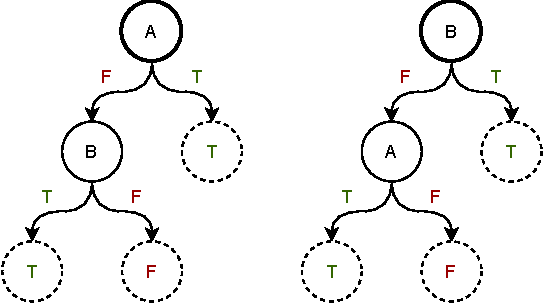
\includegraphics[scale = 0.9]{img/dt1.pdf}
    \caption{OR decision tree}
    \label{OR decision tree}
  \end{figure}
 
  \begin{figure}[h]
    \centering
    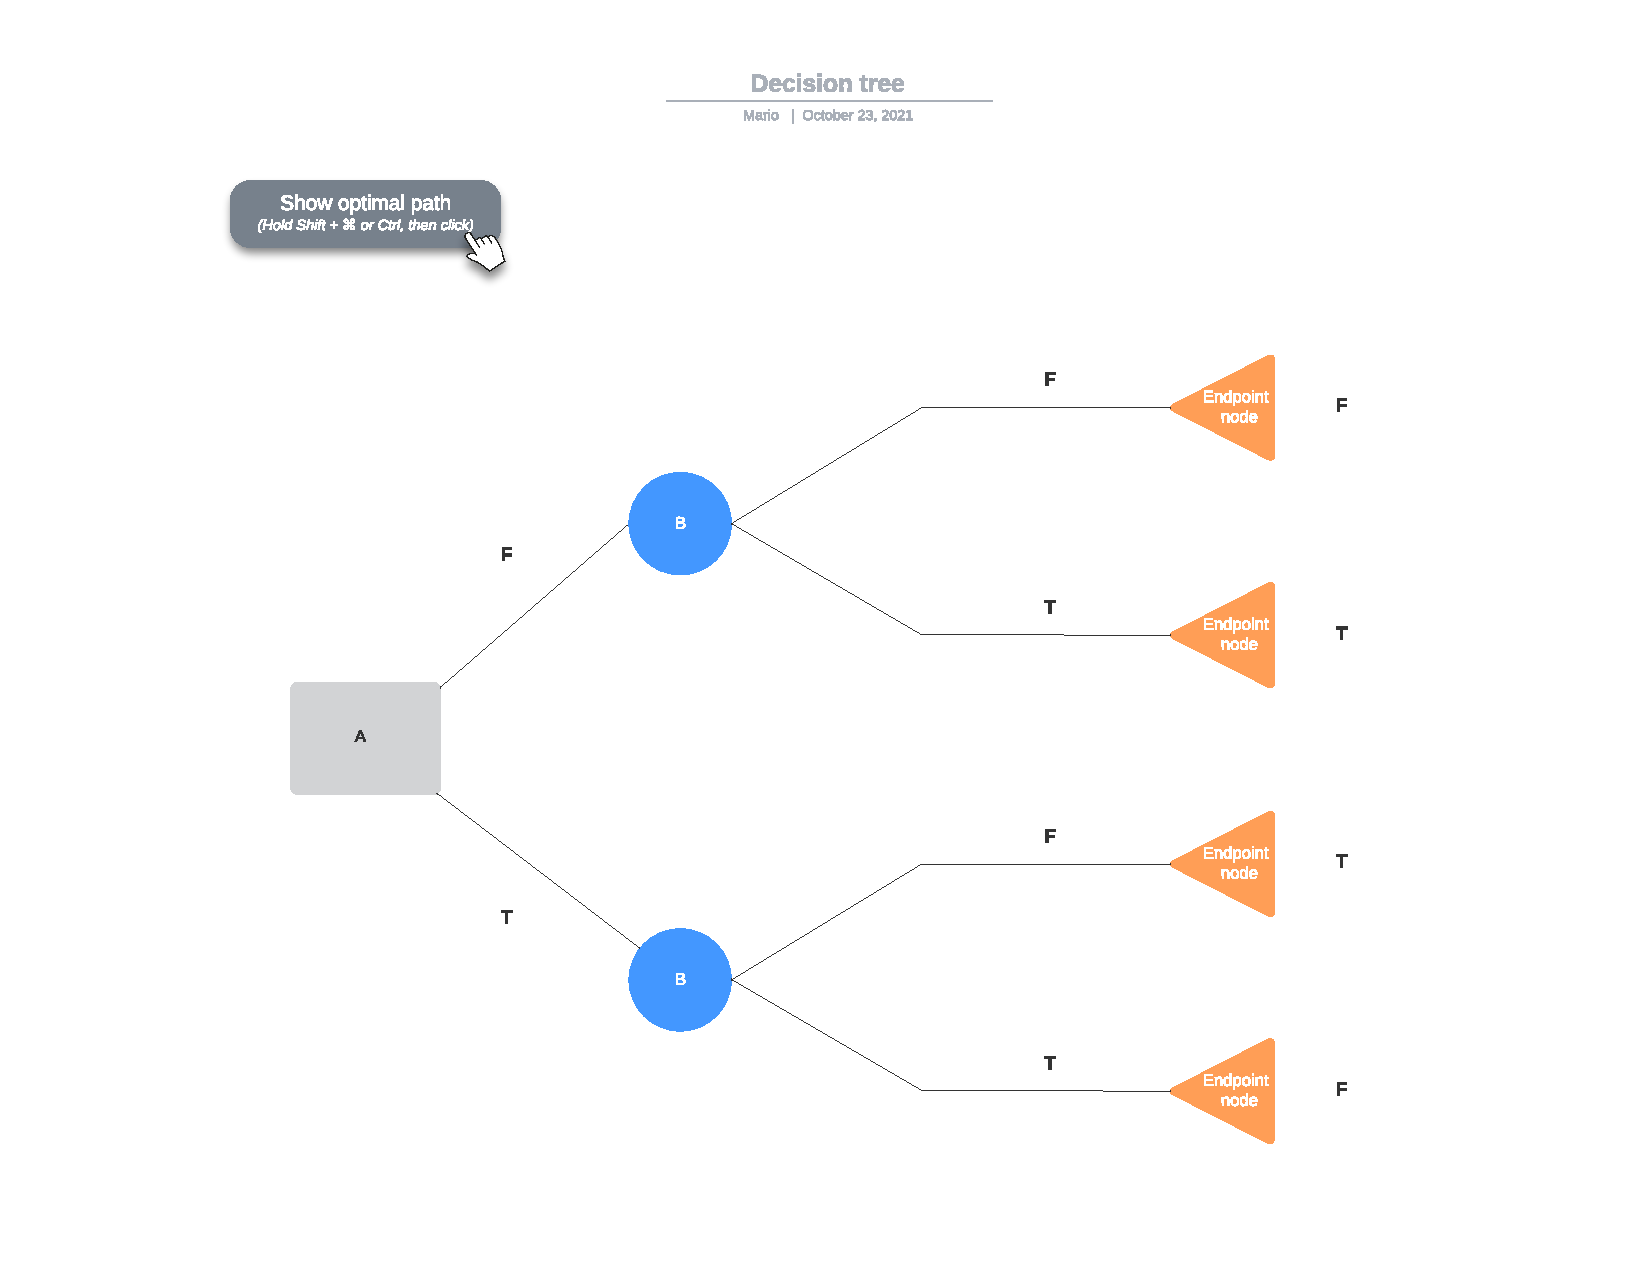
\includegraphics[scale = 0.5]{img/XOR.pdf}
    \caption{XOR decision tree}
    \label{XOR decision tree}
  \end{figure}
\end{esempio}
Essendo sempre nel concept learning, nel caso di funzioni booleane, anche il
target è booleano.
Gli alberi di decisione possono essere utilizzati anche nel continuo, per attributi numerici.
\begin{esempio}
  Immaginando  di non ritrovarci più in casi discreti ma di passare a casi \textbf{continui}. Prendiamo le istanze definite da due attributi, $x$ e $y$ e costruisco un
  albero di decisione che definisce in quali aree del piano ho $-$ e quali ho
  $+$.
  \newpage
  Si ha il seguente piano (\textbf{sull'asse delle $y$ il primo valore a partire
  dall'origine è un cinque non un sette}): 
  \begin{figure}[H]
    \centering
     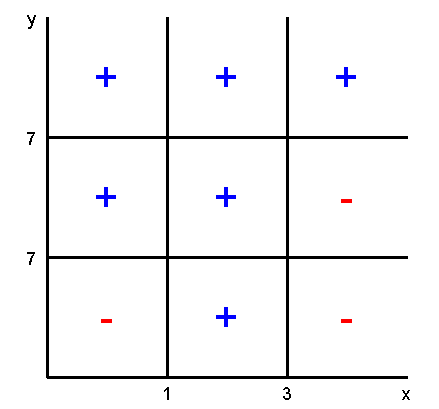
\includegraphics[scale = 0.8]{img/dt3.pdf}
  \end{figure}
  E si ottiene, per esempio, il seguente albero decisionale:
  \begin{figure}[H]
    \centering
    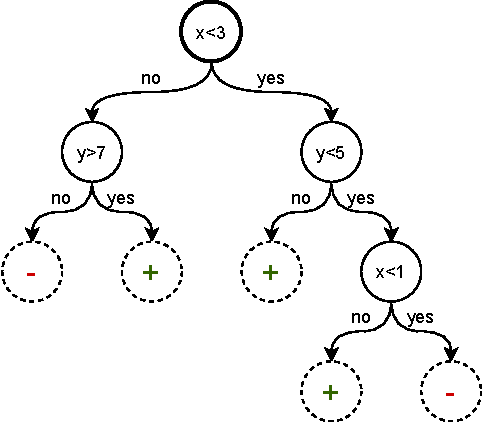
\includegraphics[scale = 0.9]{img/dt4.pdf}
  \end{figure}
  Dove a ciascun nodo è associata una condizione e agli archi il fatto che sia
  verificata o meno.\\
  Si nota come non si hanno tutte le condizioni, infatti, per esempio, con $x>3$
  mi basta $y>7$ per trovare il $+$ e $y<7$ per il $-$ (non dovendo andare
  specificatamente a guardare anche $y<5$ o $y>5$).\\
  \textbf{Quello disegnato è solo uno dei possibili alberi.}
\end{esempio}

\subsection{Algoritmo ID3}
Vista la difficoltà di scegliere l'albero si ha l'idea di scegliere un piccolo
albero di partenza (o più piccoli) e ricorsivamente l'attributo più
significativo (sia nei nodi rossi intermedi che nelle foglie) come radice per il
sotto-albero. Si fanno quindi crescere in modo 
coerente gli alberi piccoli scelti in partenza. Si punta ad arrivare a un
albero valido per tutti gli esempi ricevuti e anche per quelli non visti.\\
\begin{algorithm}[H]
  \begin{algorithmic}
    \Function{ID3}{esempi, attrib, default}
    \If{esempi è vuoto return default}
    \EndIf
    \If{tutti gli \textit{esempi} hanno la stessa classificazione \textbf{return la classificazione}}
    \EndIf
    \If{\textit{attrib} è vuoto \textbf{return VALORE\_MAGGIORANZA(esempi)}}
    \EndIf
    \State $best \gets$ \textit{il ``miglior'' attributo di decisione per il
    prossimo nodo}
    \State $albero \gets$ \textit{un nuovo albero di decisione con alla radice \textbf{best}}
    \State $m \gets$ \textit{VALORE\_MAGGIORANZA(esempi)}
    \For {\textit{ogni valore $V_i$ dell'attributo best}}
    \State $esempi \gets$ \textit{Elementi di esempi con $best = Vi$}
    \State $sottoAlb \gets$ \textit{ID3(esempi, attrib-best, m)}
    \State \textit{Aggiungi un ramo all'albero con etichetta $V_i$ e sottoalbero \textbf{sottoalb}}
    \EndFor
    \State \textit{\textbf{return albero}}
    \EndFunction
  \end{algorithmic}
  \caption{Algoritmo ID3 (Iterative Dichotomiser 3)}
\end{algorithm}
Facciamo qualche osservazione finale sull'\textbf{algoritmo ID3}:
\begin{itemize}
  \item Lo spazio delle ipotesi è completo e sicuramente contiene il target.
  \item Ho in output una singola ipotesi.
  \item Non si ha backtracking sugli attributi selezionati, si procede con una
  ricerca greedy, trovando scelte buone localmente ma non ottime.
  \item Fa scelte basate su una ricerca statistica, facendo sparire incertezze
  sui dati.
  \item Il bias non è sulla classe iniziale, essendo lo spazio delle ipotesi
  completo, ma sulla scelta di solo alcune funzioni, preferendo alberi corti (e
  più semplici) e posizionando attributi ad alto information gain vicino alla
  radice. Il bias è quindi sulla preferenza di alcune ipotesi. Si usa il
  criterio euristico di \textit{rasoio di Occam}.
  \item $H$ è l'insieme potenza delle istanze $X$.
\end{itemize}
Sfortunatamento un algoritmo scritto in questo modo è destinato a compiere qualche errore, il nostro compito sarà quello di \textbf{scoprire quanto sara scorretto}.
\section{Scegliere L'insieme degli attributi}
Ricordiamo che l'idea è quella di minimizzare la profondità dell'albero risultante. L'idea è scegliere l'attributo che fornisce la classificazione più esatta possibile degli esempi.
Bisogna in primis capire cosa si intende come \textbf{attributo migliore}.
Gli esempi positivi sono gli esempi che già mi hanno restituito \textit{yes} mentre quelli negativi sono quelli che mi hanno restituito \textit{no}.
Immaginiamo di avere un insieme di esempi $y_i$ positivi e $n_i$ negativi: \[ [y_1, y_2, y_3, y_4, n_1, n_2, n_3]\]
\begin{figure}[H]
  \centering
  \begin{tikzpicture}[nodes={draw}, -, sibling distance=100pt, level
    distance=30pt]  
    \node{\color{red} $Attributo_1$ \color{black}}
    child {node {\color{blue} $Valore_1$}
      child{node {\color{orange} $y_1, y_2, n_1, n_2$}}}
    child {node {\color{blue} $Valore_2$}
      child{node {\color{orange} $y_3, y_4, n_3$}}};
  \end{tikzpicture}
\end{figure}
La figura soprastante nostra un albero che ha come attributo $Attributo_1$ e come possibili esiti/valori di tale attributo: $Valore_1$ e $Valore_2$. Notiamo che questo attributo non è un buon attributo, poiché suddivide gli esempi in maniera \textit{mista}: l'attributo non possiede valori per cui smistare in maniera omogenea ogni singolo esempio.
\begin{figure}[H]
  \centering
  \begin{tikzpicture}[nodes={draw}, -, sibling distance=100pt, level
    distance=30pt]  
    \node{\color{red} $Attributo_2$ \color{black}}
    child {node {\color{blue} $Valore_1$}
      child{node {\color{orange} $y_1, y_2, y_3, y_4$}}}
    child {node {\color{blue} $Valore_2$}
      child{node {\color{orange} $n_1, n_2, n_3$}}};
  \end{tikzpicture}
  \label{Albero2}
\end{figure}
La figura indicata mostra invece un attributo che suddivide molto meglio gli esempi, in particolare $Valore_1$ possiede esempi positivi e $Valore_2$ esempi negativi.
\begin{definizione}
  Un attributo perfetto suddivide gli esempi in insiemi tutti positivi o tutti negativi
\end{definizione}

Ora sia Mario Avolio (autore di questa sezione di appunti) e sia voi vi chiederete "\textit{Ma come faccio a capire quanto è buono un attributo?}. In teoria la misura dovrebbe avere valore massimo quando l'attributo è perfetto e minimo quando l'attributo non è utile per nulla(tipo Windows). Una misura adeguata è la quantità attesa di \textbf{informazione} fornita dall'attributo. Essa viene misurata in \textbf{bit}. \\ Un bit d'informazione è sufficiente a rispondere $Y$ o $N$ a una domanda di cui non si sa nulla, se le possibili risposte $v_i$ hanno probabilità $P(v_i)$ allora il \textbf{contenuto informativo} $I$ della risposta corretta è dato dalla definizione di \textbf{entropia}:
\begin{definizione}
  Dato un \textbf{training set $S$} con possibili esiti sugli esempi: $v_i,\,\, i=1\ldots n$. L'entropia (fig. \ref{Entropy}) di un
  insieme di bit misura la sua quantità d'informazione (analogamente il \textbf{disordine}, ovvero il numero di elementi \textit{mischiati} tra loro, contenuto nell'insieme). In generale, se i possibili esiti $v_i,\,\, i=1\ldots n$ hanno probabilità $P(v_i)$ di essere frequenti sugli esempi, il contenuto informativo $I$ (anche chiamato \textbf{entropia}) della del training set $S$ è dato da:
  \begin{equation}
  H(P(v_1),\ldots, P(v_n))=\sum_{i=1}-P(v_i)\log_2P(v_i)
      \label{Entropy}
\end{equation}
  \end{definizione}
  \begin{figure}[H]
      \centering
      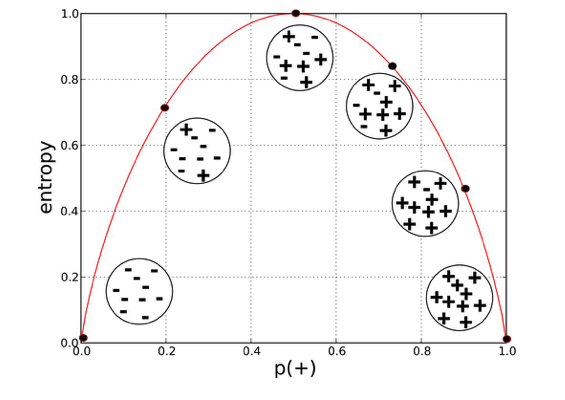
\includegraphics[width=1\textwidth]{img/entropy.png}
      \caption{Entropia al variare degli esempi \cite{}}
  \end{figure}
    Per l'apprendimento di alberi di decisione la domanda a cui vogliamo rispondere è: \textbf{dato un esempio, qual è la sua classificazione?}\\
      Per stimare la probabilità delle possibili risposte, \textbf{prima di verificare il valore degli attributi}, si può guardare la proporzione di esempi negativi e positivi nell'insieme di addestramento. Supponiamo di avere un insieme di \textbf{$p$ esempi positivi e $n$ esempi negativi}: una stima dell'informazione contenuta nella risposta corretta è:
    
      \begin{equation}
\label{Contenuto informatico di un insieme}
  I\left(\frac{p}{p+n},\frac{n}{p+n}\right)=-\frac{p}{p+n}\log_2\frac{p}{p+n}
    -\frac{n}{p+n}\log_2\frac{n}{p+n}
    \end{equation}
      
  \begin{esempio}
    Un esempio semplificato potrebbe riguardare due possibili esiti all'interno di un TrainingSet: $positivo$ e $negativo$. Se su 100 osservazioni/esempi avessimo 30 positivi e 70 negativi, allora la quantità d'informazione sarebbe:
          \begin{equation*}
  I\left(\frac{30}{100},\frac{70}{100}\right)=-\frac{30}{100}\log_2\frac{30}{100}
    -\frac{70}{100}\log_2\frac{70}{100} \approx 0.88
    \end{equation*}
  \end{esempio}

\textbf{NOTA:}
  In particolare si avrà un'alta entropia se elementi positivi e negativi sono saranno tra loro \textit{mischiati}\\
  
Il test di un singolo attributo non ci darà così tanta informazione, ma ce ne darà comunque un pò. Possiamo misurare esattamente tale quantità guardando quanta informazione ci è ancora necessaria \textit{dopo} aver effettuato il test. Ogni attributo $A$ divide l'insieme di addestramento in sottoinsiemi $E_1\dots E_v$, presupponendo che $A$ possa avere $v$ valori distinti. Ogni sottoinsieme $E_i$ ha un certo numero di esempi positivi $p_i$ e un certo numero di esempi negativi $n_i$. \\
\begin{figure}[H]
  \centering
  \begin{tikzpicture}[nodes={draw}, -, sibling distance=100pt, level
    distance=30pt]  
    \node{\color{red} $A$ \color{black}}
    child {node {\color{blue} $E_i$}
      child{node {\color{orange} $p_1 \dots p_i,\,\, n_1 \dots n_i$}}}
    child {node {\color{blue} $E_v$}
      child{node {\color{orange} $\dots$}}};
  \end{tikzpicture}
\end{figure}
Per cui se seguiamo una certa diramazione, per capire la classificazione di un esempio, avremo bisogno di un numero di bit \textbf{ulteriori} pari a:
\[I\left(\frac{p_i}{p_i+n_i},\frac{n_i}{p_i+n_i}\right)\]
Si faccia quindi riferimento alla regola \ref{Contenuto informatico di un insieme}. Un esempio preso casualmente dall'insieme di training avrà l'i-esimo valore per l'attributo con probabilità:
\[\frac{p_i+n_i}{p+n}\]
Ragion per cui, in media, dopo il test dell'attributo $A$, occorreranno ancora:
\begin{equation}
\label{IG Attributo}
remainder(A)=\sum_{i=1}^v \frac{p_i+n_i}{p+n}
  I\left(\frac{p_i}{p_i+n_i},\frac{n_i}{p_i+n_i}\right)
    \end{equation}
bit d'informazione per classificare l'esempio. Si noti che in questo caso verranno valutati tutti i valori distinti $v$ che $A$ può assumere. In particolare avremo $\frac{p_i+n_i}{p+n}$ di probabilità che $A$, in relazione ai propri possibili valori, distingui un determinato esempio.\\
Parliamo quindi di \textbf{information gain} $IG$ (in italiano: guadagno d'informazione) che viene calcolato su ogni
attributo $A$ e su $S$. In dettaglio il \textbf{guadagno d'informazione} ottenuto dal test dell'attributo è pari alla differenza tra il requisito informativo originale e quello corrente:
\begin{equation}
\label{IG}
IG(S, A)=I\left(\frac{p}{p+n},\frac{n}{p+n}\right)-remainder(A)
\end{equation}
\begin{definizione}
L'information gain è la riduzione aspettata nell'entropia per ordinare $S$ sull'attributo $A$. Si sceglie quindi l'attributo con il maggiore IG. 
\end{definizione} 
\textbf{NOTA:} la \ref{IG} è quindi sintetizzabile anche come:
\begin{equation}
\label{IG2}
IG(S, A)=Entropy(S)-\sum_{v\in values(A)}\frac{|S_v|}{|S|}Entropy(S_v)
    \end{equation}
\subsection{Approfondimento - Entropia di una Distribuzione di Probabilità}
% \begin{definizione}
%   Definiamo l'\textbf{entropia di una distribuzione condizionale}. Presa
%   una variabile aleatoria discreta $X$ con valori $\{x_1,\ldots, x_i\}$ 
%   hanno ciascuno probabilità $P(x_i)$, definiamo l'entropia 
% \begin{equation}
%   I_{Y|X=x_i}=-\sum_{j=1}^m P_{Y|X}(y_j|x_i)\cdot \log_2 P_{Y|X}(y_j|x_i)
%   \label{EntropiaDiUnaDistributzioneCondizionale}
% \end{equation}
% \textbf{NOTA:} la \ref{EntropiaDiUnaDistributzioneCondizionale} riprende la \ref{Contenuto informativo di un training set} utilizzando la probabilità condizionata.
% \end{definizione}
% \begin{definizione}
%   Definiamo \textbf{entropia condizionale} come il valore medio, ovvero il
%   valore atteso, dell'entropia di $p_{Y|X=x_i}$ per ciascun valore di $X$ che
%   condiziona $Y$, ovvero:
%   \[I_{Y|X}=\sum_{i=1}^n P_X(x_i)\cdot I_{Y|X=x_i}\]
%   ottenendo l'\textbf{entropia condizionale}:
%   \begin{equation}
%       H[Y|X]=\sum P(x)\cdot H(Y|X=x)
%         \label{EntropiaCondizionale}
%   \end{equation}
%   \textbf{NOTA:} essa si rifà alla \ref{IG Attributo}\\
%   \textbf{NOTA 2:} Si chiama \textbf{valore atteso} di una variabile aleatoria discreta il numero reale:
%   \[\sum_{k} P_X(X_k)\cdot X_k\]
%   Dove $X_k$ simboleggia il valore assunto dalla variabile $X$, mentre $P_X(X_k)$ è la sua densità. 
% \end{definizione}
Quando parliamo di \textit{entropia} stiamo volgendo un esperimento
concettuale. Prima dell'esperimento si ha una certa incertezza su un certo
evento, che sparisce, con sorpresa, una volta eseguito l'esperimento se l'evento
accade. D'altro canto qualora accadesse un evento atteso siamo meno sorpresi del
fatto (chiaramente perché sarebbe appunto "atteso"). Nel primo caso però si ritiene di ottenere molta informazione, nel
secondo caso poca. Come se ponessimo in una vasca quattro palline rosse, non
sarei stupito di estrarne una rossa, essendo quello che mi aspetto. D'altro
canto se ne aggiungo quattro verdi l'estrazione sarà inattesa e quindi più
interessante.\\ 
Si cerca un modo di quantificare questa ``sorpresa''. Riprendendo l'esempio
delle palline posso dire che nel primo caso (solo rosse) ho \textbf{bassa
  entropia/basso contenuto informativo} e nel secondo caso (palline miste) \textbf{alta entropia/alto contenuto informativo}. Un caso
intermedio sarebbe a \textbf{media entropia}.\\
Sia $P(x)$ la probabilità che avvenga un evento $x$ e sia $H(p)$ l'informazione (entropia) che ottengo dopo che l'evento si è verificato:
\begin{itemize}
  \item $P(x)=1\to H(p)=0$
  \item $P(x)=0\to H(p)=\infty$
\end{itemize}
L'informazione $H(p)$ e quindi una quantità non negativa:
\[H(p)\geq 0\]
Definiamo quindi l'informazione, detta anche \textit{self-information}, per un
evento $E$: 
\[H(E)=-\log_2(P(E))\]
Inoltre si può affermare che essa disponga della proprietà additiva se gli eventi sono indipendenti, ovvero:
\[H(p_1, p_2)=H(p_1)+H(p_2)\]

  L'\textbf{entropia}, definita da Claude Shannon (e quindi spesso chiamata
  \textbf{entropia di Shannon}), è l'informazione media associata ad
  una distribuzione di probabilità.\\
\begin{definizione}
Sia $X$ una variabile aleatoria che può assumere valori pari a ${x_1 \dots x_n}$ con probabilità $p_i$ analogamente a quanto detto nel precedente paragrafo possiamo calcolarne l'\textbf{entropia}, ovvero il \textbf{contenuto informativo}:
\begin{equation}
    H[X]=-\sum_{i=1}^n p_i\cdot\log_2 p_i
\label{EntropiaVariabile}
\end{equation}
\end{definizione}
Analogamente a quanto visto per un dataset, si può vedere una variabile aleatoria discreta $X$ ( quindi una distribuzione di probabilità ) come un vero e proprio dataset. Didatti si noti che la \ref{EntropiaVariabile} è identica alla \ref{Entropy}
\subsubsection{Entropia Condizionata}
Analogamente a quanto visto per la \ref{EntropiaVariabile} possiamo chiaramente sfruttare una distribuzione \textbf{condizionale} di probabilità. Ovvero possiamo sfruttare la \textbf{probabilità condizionata}. Per arrivare al concetto di \textbf{entropia condizionale} di un'intera variabile aleatoria $X$ (che supponiamo possa assumere $x_n$ valori) dobbiamo passare per un concetto intermedio. I lettori di questo libro sicuramente si ricorderanno che negli scorsi paragrafi abbiamo detto che:  
\begin{displayquote}
Ogni attributo $A$ divide l'insieme di addestramento in sottoinsiemi $E_1\dots E_v$, presupponendo che $A$ possa avere $v$ valori distinti. Ogni sottoinsieme $E_i$ ha un certo numero di esempi positivi $p_i$ e un certo numero di esempi negativi $n_i$. Per cui se seguiamo una certa diramazione, per capire la classificazione di un esempio, avremo bisogno di un numero di bit \textbf{ulteriori} pari a:
\[I\left(\frac{p_i}{p_i+n_i},\frac{n_i}{p_i+n_i}\right)\]
\end{displayquote}
Analogamente ora andremo a definire l'entropia di una variabile aleatoria discreta $Y$ condizionata dall'evento $X=x_i$, ovvero dall'evento che $X$ assuma un determinato valore. In questo caso particolare $A=X$ e $E_1 \dots E_v = x_1 \dots x_i$.
\begin{definizione}
Sia $Y$ una variabile aleatoria e $X=x_i$ l'evento che la coinvolge, allora si può descrivere l'entropia come:
  \begin{equation}
    H_{Y|X=x_i}=-\sum_{j=1}^m P_{Y|X}(y_j|x_i)\cdot\log_2 P_{Y|X}(y_j|x_i)
\label{EntropiaCondizionaleParziale}
\end{equation}
\end{definizione}
Tale equazione ci permette di definire l'entropia solo nel caso in cui un \textbf{attributo} o una \textbf{variabile aleatoria} $X$ assumano un valore $x_i$. 
\textbf{L'entropia condizionale} quantifica invece la quantità d'informazione di cui si ha bisogno per descrivere l'esito di una \textbf{variabile aleatoria} $Y$ data un'\textbf{intera} variabile aleatoria $X$. In particolare essa riprende il risultato della media di $H_{Y|X=x_i}$ per tutti i possibili valori che $X$ può assumere. 
Ricordiamo ora la quantità di bit d'informazione necessari per classificare un attributo:
\begin{displayquote}
Ragion per cui, in media, dopo il test dell'attributo $A$, occorreranno ancora:
\begin{equation}
\label{IG Attributo}
remainder(A)=\sum_{i=1}^v \frac{p_i+n_i}{p+n}
  I\left(\frac{p_i}{p_i+n_i},\frac{n_i}{p_i+n_i}\right)
    \end{equation}
bit d'informazione per classificare l'esempio. Si noti che in questo caso verranno valutati tutti i valori distinti $v$ che $A$ può assumere. In particolare avremo $\frac{p_i+n_i}{p+n}$ di probabilità che $A$, in relazione ai propri possibili valori, distingui un determinato esempio.
\end{displayquote}
Forniamo una definizione equivalente mediante \textbf{l'entropia condizionale}:
\begin{definizione}
Date due variabile aleatoria discrete $X$ e $Y$, l'\textbf{entropia condizionale} di $Y$ dato $X$ è definita come la somma ponderata di $H_{Y|X=x_i}$ per ogni possibile valore di $x_i$, usando $p(xi)$ come peso:
  \begin{equation}
    H_{Y|X}=\sum_{x_i\in X} p(x_i)\cdot H_{Y|X=x_i}
    \label{EntropiaCondizionale}
\end{equation}
\end{definizione}

\section{Valutare le prestazioni dell'algoritmo di apprendimento}
\begin{definizione}
  Un algoritmo di apprendimento è buono se produce ipotesi che riescono a predire con accuratezza la classificazione di esempi mai incontrati precedentemente.
\end{definizione}
Una predizione viene valutata in relazione a un \textbf{insieme di test}. Per questo motivo solitamente è doveroso adottare tale strategia:
\begin{enumerate}
    \item Raccogliere un grande insieme di test.
    \item Dividerlo in due insiemi disgiunti: uno per l'addestramento e uno per i test
    \item Applicare l'algoritmo di apprendimento all'insieme di addestramento, generando un'ipotesi $h$ (come già visto nel precedente capitolo sul Concept Learning)
    \item Misurare la percentuale di esempi nell'insieme di test che vengono classificati correttamente da $h$.
    \item Ripetere i passi 2 e 4 con dimensioni e insiemi diverse degli insiemi di addestramento.
\end{enumerate}
Il risultato di quanto descritto è un insieme di dati che può essere elaborato per fornire la qualità media della predizione in funzione delle dimensioni dell'insieme di addestramento. Questa funzione si può tracciare su un grafico, ottenendo la \textbf{curva di apprendimento}. \\ In questo contesto è opportuno evitare ciò che viene chiamato \textbf{peeking}: \textit{andare a creare un'ipotesi (NON generale) in base a un insieme di test che viene controllato a priori (e non a posteriori come si dovrebbe fare con dei test appunto).}
\section{Rumore e sovradattamento}
\subsection{Rumore}
Come abbiamo visto precedentemente, qualora due o più esempi contenessero la stessa descrizione ma avessero descrizioni differenti, l'algoritmo \textbf{IG3} non riuscirà a trovare un albero consistente per tutti gli esempi proposti. Una semplice soluzione per risolvere il problema è quella di far restituire a ogni nodo foglia la classificazione di maggioranza per il suo insieme di esempi. Questo solitamente porta a problemi poiché l'algoritmo genera un albero consistente per tutti gli esempi considerando quei attributi \textbf{irrilevanti} per operare distinzioni spurie tra gli esempi. 
\subsection{Overfitting}
Ogniqualvolta si opera con un insieme vasto d'ipotesi occorre stare attenti a non ricadere nell'\textbf{overfitting}(sovradattamento).
\begin{definizione}
  \textit{Definizione tratta da Wikipedia.}\\
  Definiamo formalmente l'\textbf{overfitting} come l'adattamento eccessivo,
  ovvero quando 
  un modello statistico molto complesso si adatta al campione perché ha un
  numero eccessivo di parametri rispetto al numero di osservazioni. SI ha
  quindi che un modello assurdo e sbagliato può adattarsi perfettamente se è
  abbastanza complesso rispetto alla quantità di dati disponibili.\\
  Nel machine learning se il learner viene addestrato troppo a lungo il modello
  potrebbe adattarsi a caratteristiche che sono specifiche solo del training
  set, ma che non hanno riscontro nel resto dei casi quindi le prestazioni sui
  dati non visionati saranno drasticamente peggiori.\\
  L'opposto è l'\textbf{underfitting}.
\end{definizione}

Se misuro l'errore di una ipotesi
$h$ sul training set ($error_{traini}(h)$) e poi misuro l'errore di quella
ipotesi sull'intero set delle possibili istanze
$D$ ($error_D(h)$) ho che l'ipotesi $h$ va in \textbf{overfit} sul quel data set
se:
\[error_{traini}(h) < error_{traini}(h') \,\,\land
  \,\, error_D(h)>error_D(h')\]
quindi se presa un'altra ipotesi questa è migliore della prima e ha un errore
sull'intera distribuzione delle ipotesi inferiore vado in \textit{overfit}. Il
problema è che non posso sapere se esiste tale $h'$. Per evitare il problema uso
sempre il rasoio di Occam scegliendo ipotesi semplici ed evitando di far
crescere l'albero quando lo ``split'' non è statisticamente significativo. Un
altro modo è quello di togliere pezzi, all'albero, che toccano poche istanze o
pure calcolare una \textit{misura di complessità dell'albero}, minimizzando la
grandezza dell'albero e gli errori del \textit{training set}, usando il
\textbf{Minimum Description Length (\textit{MDL})}.\\
In ID3 quindi posso scegliere sia in base all'\textit{information gain} massimo
o all'\textit{entropia} minima tra gli attributi.\\
Come specificato, una metodologia semplice da poter applicare in queste situazioni riguarda la \textbf{potatura dell'albero di decisione}. Essa opera impedendo la divisione ricorsiva su attributi che non sono chiaramente rilevamenti, anche quando i dati di un determinato nodo non sono classificati in modo uniforme. I lettori di questi appunti a questo punto si chiederanno sicuramente la seguente domanda: "Mario, se l'irrilevanza di un attributo si misura in relazione alla sua informazione fornita, quanto deve valere quest'ultima per etichettare un nodo come 'irrilevante'?". Per rispondere a questa domanda possiamo ricorrere a un \textbf{test di significatività} statistico: si comincia con un'\textbf{ipotesi nulla}, ovvero che l'attributo sia irrilevante; quindi i dati vengono analizzati per calcolare quanto si discostano effettivamente dalla totale assenza di pattern nei confronti degli esempi. Se il grado di derivazione risulta improbabile, questo viene considerato un buon indizio della presenza di un pattern significativo nei dati. \\ Un'altra possibile opzione da tenere in considerazione (magari insieme alla potatura) è la \textbf{validazione incrociata}: stimare quanto bene ogni ipotesi potrà predire dati mai incontrati.
\section{Esercizi Guidati}
\begin{esempio}
  Suppongo di lanciare una moneta, si ha:
  \[P(testa)=P(croce)=\frac{1}{2}\]
  Definiamo che testa è specificata da $X=0$ e croce da $X=1$.\\
  Calcoliamo quindi:
  \[H(p)=-p(0)\cdot \log_2 p(0)-p(1)\cdot\log_2
    p(1)=-2\cdot(\frac{1}{2}\cdot\log_2\frac{1}{2})=1\] 
  Una moneta ``onesta'' ha quindi entropia pari a 1 (avendo due probabili esiti
  equiprobabili non ho certezza del risultato).\\
  Ipotizziamo di avere una moneta magica che cade solo sulla testa (quindi
  $P(0)=1$ e $P(1)=0$:
  \[H(p)=-p(0)\cdot \log_2 p(0)-p(1)\cdot\log_2 p(1)=-\log_2 (1)=0\]
  Una moneta ``non onesta'' ha quindi entropia pari a 0 (ho infatti certezza del
  risultato).
\end{esempio}
\begin{esempio}
  Considero il seguente training set, con 4 esempi e target $T$:
  \begin{table}[H]
    \centering
    \begin{tabular}{c|c|c|c|c|c}
      example & A & B & C & D & T\\
      \hline
      $x_1$ & 0 & 0 & 1 & 1 & \color{darkgreen}{1}\\
      $x_2$ & 0 & 1 & 1 & 1 & \color{darkgreen}{1}\\
      $x_3$ & 0 & 1 & 0 & 0 & \color{red}{0}\\
      $x_4$ & 0 & 1 & 0 & 1 & \color{darkgreen}{1}\\
    \end{tabular}
  \end{table}
  Si ha quindi la seguente distribuzione di probabilità relativa al target
  (avendo un \textit{no} e tre \textit{yes}):
  \[P_T=\left[\frac{1}{4},\frac{3}{4}\right]\]
  e quindi posso calcolare l'entropia della tabella, ovvero il contenuto informatico $H$ dato dalla distribuzione di probabilità del target $T$ (che sarebbe la nostra variabile aleatoria $X$).
  \[H(P_T)=-P_T(0)\cdot \log_2 P_T(0)-P_T(1)\cdot\log_2
    P_T(1)=-\frac{1}{4}\cdot\log_2\frac{1}{4}-\frac{3}{4}\cdot\log_2
    \frac{3}{4}= 0.81\]
    Tramite essa siamo riusciti a calcolare il contenuto informativo del DataSet.
\textbf{  Passiamo ora all'uso d'iD3 per la costruzione dell'albero. Dobbiamo cercare gli split corretti tramite information gain, usando
  l'entropia condizionale.\\}
  Partiamo con il primo attributo: $A$.\\ Si ha che $P_A(0)=1$ e $P_A(1)=0$,
  quindi, seguendo la \ref{EntropiaCondizionaleParziale}:
  \[H[T|A=0]=-p_{T|A}(0|0)\cdot \log_2(p_{T|A}(0|0))-p_{T|A}(1|0)\cdot
    \log_2(p_{T|A}(1|0))=\]
  \[-\frac{1}{4}\cdot\log_2\frac{1}{4}-
    \frac{3}{4}\cdot\log_2\frac{3}{4}=0.81\]
  (Risultato pari a quello dell'intero training set in quanto $A$ è sempre 0)\\
  Non devo calcolare $H[T|A=1]$ in quanto $A$ non è mai pari ad 1.\\
  A questo punto è doveroso calcolare \textbf{l'entropia condizionale} per l'attributo $A$ (che in questo caso sarebbe la variabile aleatoria $X$) seguendo la \ref{EntropiaCondizionale}:
  \[H[T|A]=P_A(0)\cdot H[T|A=0]+P_A(1)\cdot H[T|A=1]=1\cdot 0.81=0.81\]
  Posso quindi calcolare l'\textit{information gain} secondo la \ref{IG}:
  \[IG[T;A]=H[T]-H[T|A]=0.81-0.81=0\]
  Quindi per $A$ ho la seguente distribuzione del target (avendo nel target 3
  esempi positivi e uno negativo e $A$ sempre con valore 0):
  \begin{figure}[H]
    \centering
    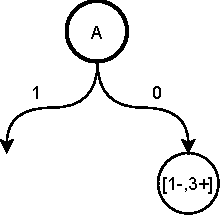
\includegraphics[scale = 0.9]{img/id1.pdf}
  \end{figure}
 \textbf{\textit{Ricordiamo che ID3 sceglie per lo splitting l'attributo che
     rende massimo l'information gain.}}\\
  Passo quindi all'attributo $B$. Si ha che $P_B(0)=\frac{1}{4}$ e
  $P_B(1)=\frac{3}{4}$, quindi:
  \[H[T|B=0]=-p_{T|B}(0|0)\cdot \log_2(p_{T|B}(0|0))-p_{T|B}(1|0)\cdot
    \log_2(p_{T|B}(1|0))=\]
  \[-0\cdot \log_2 0-1\cdot \log_2 1=0\]
  e:
  \[H[T|B=1]=-p_{T|B}(0|1)\cdot \log_2(p_{T|B}(0|1))-p_{T|B}(1|1)\cdot
    \log_2(p_{T|B}(1|1))=\]
  \[-\frac{1}{3}\cdot\log_2\frac{1}{3}-
    \frac{2}{3}\cdot\log_2\frac{2}{3}=0.91\]
  (ho quindi una partizione migliore con $B=0$)\\
  Inoltre si ha:
  \[H[T|B]=P_B(0)\cdot H[T|B=0]+P_B(1)\cdot H[T|B=1]=\frac{1}{4}\cdot
    0+\frac{3}{4}\cdot 0.91=0.68\]
  Posso quindi calcolare l'\textit{information gain}:
  \[IG[T;B]=H[T]-H[T|B]=0.81-0.68=0.13\]
  Quindi per $B$ ho:
  \begin{figure}[H]
    \centering
    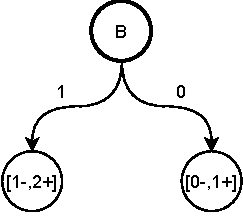
\includegraphics[scale = 0.9]{img/id2.pdf}
  \end{figure}
  Ho quindi un partizionamento più interessante.\\
  Passo quindi all'attributo $C$. Si ha che $P_C(0)=\frac{1}{2}$ e
  $P_C(1)=\frac{1}{2}$, quindi:
  \[H[T|C=0]=-p_{T|C}(0|0)\cdot \log_2(p_{T|C}(0|0))-p_{T|C}(1|0)\cdot
    \log_2(p_{T|C}(1|0))=\]
  \[-\frac{1}{2}\cdot \log_2 \frac{1}{2}-\frac{1}{2}\cdot \log_2 \frac{1}{2}=1\]
  e:
  \[H[T|C=1]=-p_{T|C}(0|1)\cdot \log_2(p_{T|C}(0|1))-p_{T|C}(1|1)\cdot
    \log_2(p_{T|C}(1|1))=\]
  \[-0\cdot \log_2 0-1\cdot \log_2 1=0\]
  Inoltre si ha:
  \[H[T|C]=P_C(0)\cdot H[T|C=0]+P_C(1)\cdot H[T|C=1]=\frac{1}{2}\cdot
    1+\frac{1}{2}\cdot 0=\frac{1}{2}\]
  Posso quindi calcolare l'\textit{information gain}:
  \[IG[T;C]=H[T]-H[T|C]=0.81-\frac{1}{2}=0.31\]
  Quindi per $C$ ho:
  \begin{figure}[H]
    \centering
    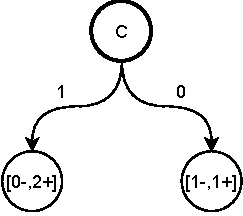
\includegraphics[scale = 0.9]{img/id3.pdf}
  \end{figure}
  $C$ migliora ancora il partizionamento.\\
  Passo quindi all'attributo $D$. Si ha che $P_D(0)=\frac{1}{4}$ e
  $P_D(1)=\frac{3}{4}$, quindi:
  \[H[T|D=0]=-p_{T|D}(0|0)\cdot \log_2(p_{T|D}(0|0))-p_{T|D}(1|0)\cdot
    \log_2(p_{T|D}(1|0))=\]
  \[-1\cdot \log_2 1-0\cdot \log_2 0=0\]
  e:
  \[H[T|D=1]=-p_{T|D}(0|1)\cdot \log_2(p_{T|D}(0|1))-p_{T|D}(1|1)\cdot
    \log_2(p_{T|D}(1|1))=\]
  \[-0\cdot \log_2 0-1\cdot \log_2 1=0\]
  Inoltre si ha:
  \[H[T|D]=P_D(0)\cdot H[T|D=0]+P_D(1)\cdot H[T|D=1]=\frac{1}{4}\cdot
    0+\frac{3}{4}\cdot 0=0\]
  Posso quindi calcolare l'\textit{information gain}:
  \[IG[T;D]=H[T]-H[T|D]=0.81-0=0.81\]
  Quindi per $D$ ho:
  \begin{figure}[H]
    \centering
    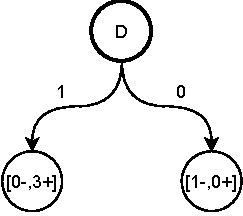
\includegraphics[scale = 0.9]{img/id4.pdf}
  \end{figure}
  $D$ rende quindi il massimo della ``purezza'' tra i valori di $D$ e quelli del
  target. Non si ha incertezza nel partizionamento e non siamo sorpresi da esso.\\
  Quindi, ricapitolando, ho i seguenti information gain:
  \begin{itemize}
    \item $IG[T;A]=0$
    \item $IG[T;B]=0.13$
    \item $IG[T;C]=0.31$
    \item $IG[T;D]=0.81$, \textbf{che è il valore massimo} e che rende minima la
    ``sorpresa''
  \end{itemize}
\end{esempio}
\begin{esempio}
  Considero il seguente training set, con 4 esempi e target $T$:
  \begin{table}[H]
    \centering
    \begin{tabular}{c|c|c|c|c|c}
      example & A & B & C & D & T\\
      \hline
      $x_1$ & 0 & 0 & 1 & $\ldots$ & \color{darkgreen}{1}\\
      $x_2$ & 0 & 1 & 1 & $\ldots$ & \color{darkgreen}{1}\\
      $x_3$ & 0 & 1 & 0 & $\ldots$ & \color{red}{0}\\
      $x_4$ & 0 & 1 & 0 & $\ldots$ & \color{darkgreen}{1}\\
    \end{tabular}
  \end{table}
  Bisogna riempire $D$ per rendere massimo l'information gain.
  \newpage
  Per farlo basta mettere gli stessi valori del target, in modo che sia
  l'attributo che meglio distribuisca i valori del target, ottenendo quindi lo
  stesso training set dell'esempio precedente:
  \begin{table}[H]
    \centering
    \begin{tabular}{c|c|c|c|c|c}
      example & A & B & C & D & T\\
      \hline
      $x_1$ & 0 & 0 & 1 & 1 & \color{darkgreen}{1}\\
      $x_2$ & 0 & 1 & 1 & 1 & \color{darkgreen}{1}\\
      $x_3$ & 0 & 1 & 0 & 0 & \color{red}{0}\\
      $x_4$ & 0 & 1 & 0 & 1 & \color{darkgreen}{1}\\
    \end{tabular}
  \end{table}
  Un'alternativa è l'esatto opposto, in quanto otterrei la stessa
  ridistribuzione del target, rimuovendo ogni ``sorpresa'' ulteriore ma
  lasciando solo quella della tabella iniziale:
  \begin{table}[H]
    \centering
    \begin{tabular}{c|c|c|c|c|c}
      example & A & B & C & D & T\\
      \hline
      $x_1$ & 0 & 0 & 1 & 0 & \color{darkgreen}{1}\\
      $x_2$ & 0 & 1 & 1 & 0 & \color{darkgreen}{1}\\
      $x_3$ & 0 & 1 & 0 & 1 & \color{red}{0}\\
      $x_4$ & 0 & 1 & 0 & 0 & \color{darkgreen}{1}\\
    \end{tabular}
  \end{table}
\end{esempio}
\begin{esempio}
  Considero il seguente training set, con 4 esempi e target $T$:
  \begin{table}[H]
    \centering
    \begin{tabular}{c|c|c|c|c}
      example & $f_1$ & $f_2$ & $f_3$ & T\\
      \hline
      $x_1$ & 1 & 1 & 1 & \color{darkgreen}{1}\\
      $x_2$ & 0 & 1 & 1 & \color{red}{0}\\
      $x_3$ & 0 & 0 & 1 & \color{darkgreen}{1}\\
      $x_4$ & 0 & 0 & 0 & \color{red}{0}\\
    \end{tabular}
  \end{table}
  Vogliamo completare il seguente albero decisionale:
  \begin{figure}[H]
    \centering
    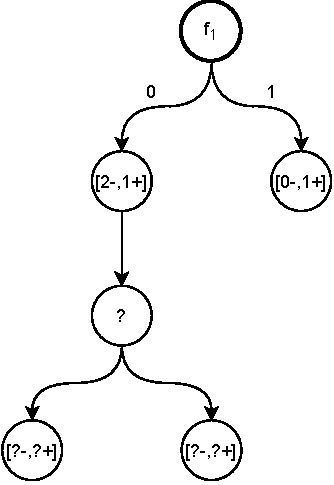
\includegraphics[scale = 0.75]{img/id5.pdf}
  \end{figure}
  Partendo da $f_1$ so che se arriva un nuovo esempio non potrò proseguire da
  $[0-, 1+]$ in quanto so già che in quel caso avrei un'istanza positiva, valore
  minimo $0$.\\
  Quindi se $f_1=0$ vado a scegliere un nuovo attributo in quanto ancora non ho
  una distribuzione certa.\textbf{ Considero quindi le righe in cui $f_1=0$} e avanzo
  iterativamente studiando $f_2$ ed $f_3$. Studio quindi il sottoinsieme: 
  \begin{table}[H]
    \centering
    \begin{tabular}{c|c|c|c}
      example  & $f_2$ & $f_3$ & T\\
      \hline
      $x_2$ & 1 & 1 & \color{red}{0}\\
      $x_3$ & 0 & 1 & \color{darkgreen}{1}\\
      $x_4$ & 0 & 0 & \color{red}{0}\\
    \end{tabular}
  \end{table}
  e avanzo fino a che non finisco gli attributi (o arrivo in un punto in cui,
  come per il ramo 1 di $f_1$ non posso più continuare).\\
  Per questo nuovo sottoinsieme calcolo:
  \[P_T=\left[\frac{2}{3},\frac{1}{4}\right]\]
  e quindi posso calcolare l'entropia della tabella:
  \[H(P_T)=-P_T(0)\cdot \log_2 P_T(0)-P_T(1)\cdot\log_2
    P_T(1)=-\frac{2}{3}\cdot\log_2\frac{2}{3}-\frac{1}{3}\cdot\log_2
    \frac{1}{3}= 0.91\]
  Passo quindi all'attributo $f_2$. Si ha che $P_{f_2}(0)=\frac{2}{3}$ e
  $P_{f_2}(1)=\frac{1}{3}$, quindi:
  \[H[T|f_2=0]=-p_{T|f_2}(0|0)\cdot \log_2(p_{T|f_2}(0|0))-p_{T|f_2}(1|0)\cdot
    \log_2(p_{T|f_2}(1|0))=\]
  \[-\frac{1}{2}\cdot \log_2 \frac{1}{2}-\frac{1}{2}\cdot \log_2 \frac{1}{2}=1\]
  e:
  \[H[T|f_2=1]=-p_{T|f_2}(0|1)\cdot \log_2(p_{T|f_2}(0|1))-p_{T|f_2}(1|1)\cdot
    \log_2(p_{T|f_2}(1|1))=\]
  \[-0\cdot \log_2 0-1\cdot \log_2 1=0\]
  Inoltre si ha:
  \[H[T|f_2]=P_{f_2}(0)\cdot H[T|f_2=0]+P_{f_2}(1)\cdot
    H[T|f_2=1]=\frac{2}{3}\cdot 1+\frac{1}{3}\cdot 0=\frac{2}{3}\]
  Posso quindi calcolare l'\textit{information gain}:
  \[IG[T;f_2]=H[T]-H[T|f_2]=0.81-\frac{2}{3}=0.25\]
  
  Passo quindi all'attributo $f_3$. Si ha che $P_{f_3}(0)=\frac{1}{3}$ e
  $P_{f_3}(1)=\frac{2}{3}$, quindi:
  \[H[T|f_3=0]=-p_{T|f_3}(0|1)\cdot \log_2(p_{T|f_3}(0|1))-p_{T|f_3}(1|1)\cdot
    \log_2(p_{T|f_3}(1|1))=\]
  \[-1\cdot \log_2 1-0\cdot \log_2 0=0\]
  e:
  \[H[T|f_3=1]=-p_{T|f_3}(0|0)\cdot \log_2(p_{T|f_3}(0|0))-p_{T|f_3}(1|0)\cdot
    \log_2(p_{T|f_3}(1|0))=\]
  \[-\frac{1}{2}\cdot \log_2 \frac{1}{2}-\frac{1}{2}\cdot \log_2 \frac{1}{2}=1\]
  Inoltre si ha:
  \[H[T|f_3]=P_{f_3}(0)\cdot H[T|f_3=0]+P_{f_3}(1)\cdot
    H[T|f_3=1]=\frac{1}{3}\cdot 0+\frac{2}{3}\cdot 1=\frac{2}{3}\]
  Posso quindi calcolare l'\textit{information gain}:
  \[IG[T;f_3]=H[T]-H[T|f_3]=0.81-\frac{2}{3}=0.25\]
  Avendo $f_2$ e $f_3$ lo stesso $IG$ prendo il primo e quindi ho:
  \begin{figure}[H]
    \centering
    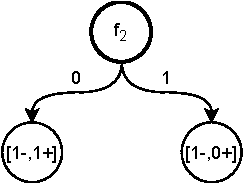
\includegraphics[scale = 0.9]{img/id6.pdf}
  \end{figure}
  Con $f_2$ che verrà attaccato al nodo $[2-, 1+]$ ``uscente'' da $f_1$.\\
 \textbf{ A questo punto, come sopra, abbiamo che il nodo $[1-, 0+]$ è foglia, avendo una
  distribuzione certa}. Riduco quindi nuovamente il training set studiando solo
  gli esempi in cui $f_2$ vale 0, ovvero $x_3$ e $x_4$, per l'attributo $f_3$;
  \begin{table}[H]
    \centering
    \begin{tabular}{c|c|c}
      example & $f_3$ & T\\
      \hline
      $x_3$ & 1 & \color{darkgreen}{1}\\
      $x_4$ & 0 & \color{red}{0}\\
    \end{tabular}
  \end{table}
  \newpage
  Non sono necessari conti in quanto $f_3$ è l'ultimo attributo rimasto ed è
  distribuito in questo modo:
  \begin{figure}[H]
    \centering
    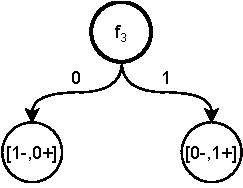
\includegraphics[scale = 0.9]{img/id7.pdf}
  \end{figure}
  Avendo per di più entrambi i risultati con distribuzione certa.\\
  Il nodo di $f_3$ sarà attaccato al nodo $[1-, 1+]$ ``uscente'' da $f_2$,
  ottenendo così l'albero:
  \begin{figure}[H]
    \centering
    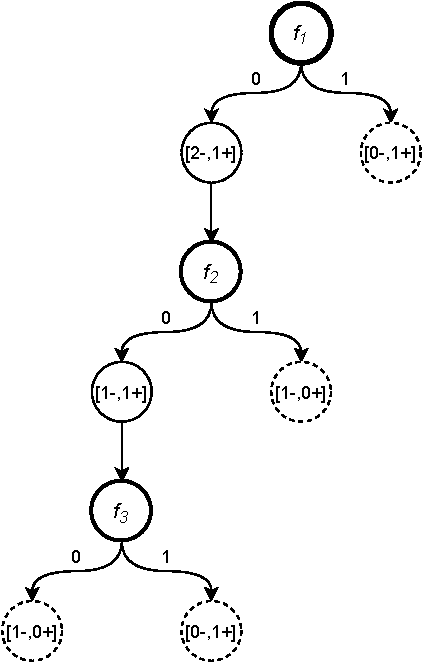
\includegraphics[scale = 1]{img/id8.pdf}
  \end{figure}
\end{esempio}
% \section{Considerazioni Finali}
% Arrivati a questo punto è necessario fare un resoconto finale su come costruire un albero partendo da un Training Set.
% \begin{enumerate}
%     \item Calcolo dell'entropia del Training Set (\ref{Contenuto informatico di un insieme} o \ref{Contenuto informativo di un training set}):
%     \[I\left(\frac{p}{p+n},\frac{n}{p+n}\right)=-\frac{p}{p+n}\log_2\frac{p}{p+n}
%     -\frac{n}{p+n}\log_2\frac{n}{p+n}\]
    
%     \item Calcolo delle probabilità del primo attributo in tabella disponibile:
%     \[\frac{p_i+n_i}{p+n}\]

%     \item Calcolo l'entropia/contenuto informativo dell'attributo:
%         \begin{enumerate}
%             \item In Generale avremo:
%             \[I\left(\frac{p_i}{p_i+n_i},\frac{n_i}{p_i+n_i}\right)\]
            
%             \item Se si parla di probabilità condizionata, dalla precedente formula si deriva:
%             \[I_{Y|X=x_i}=-\sum_{j=1}^m P_{Y|X}(y_j|x_i)\cdot \log_2 P_{Y|X}(y_j|x_i)\]
%         \end{enumerate}
    
%     \item Calcolo il $Resto(A)$
%         \begin{enumerate}
%           \item In generale si opta per:
%             \[remainder(A)=\sum_{i=1}^v \frac{p_i+n_i}{p+n}
%   I\left(\frac{p_i}{p_i+n_i},\frac{n_i}{p_i+n_i}\right)\]
          
%             \item In caso di probabilità condizionata la formula si riduce alla \ref{EntropiaCondizionale}:
%                   \[H[Y|X]=\sum P(x)\cdot H(Y|X=x)\]
%         \end{enumerate}
          
%     \item Calcolo IG :
%             \[IG(S,A)=I\left(\frac{p}{p+n},\frac{n}{p+n}\right)-remainder(A)\]
% \end{enumerate}

%3

%---------- Reti Neurali ----- 
\chapter{Reti neurali}
\label{Capitolo 4}
%%%%%%%%%%%%%%%%%%%%%%%%%%%%%%%%%%%%%%%%%%%%55
%%%%%%%%%%%%%%%%%%%%%%%%%%%%%%%%5

In natura l'operazione di \textit{learning} viene eseguita tramite il
\textbf{cervello}, che tramite i \textbf{neuroni}, delle cellule nervose, è in
grado di effettuare una miriade di operazioni in parallelo. Potenzialmente i
neuroni hanno un tempo di risposta nell'ordine dei millisecondi mentre in
circuito logico si aggira nell'ordine dei nanosecondi quindi la differenza deve
essere ricercata nell'\textit{architettura} del nostro cervello. La ``potenza di
calcolo'' del cervello è data dal funzionamento parallelo di $\sim 10^{11}$
neuroni, collegati tra loro da $\sim 10^5$ connessioni. Vediamo quindi
indicativamente gli elementi principali di un \textbf{neurone biologico}:
\begin{itemize}
	\item \textbf{corpo}, che implementa tutte le funzioni logiche del neurone
	\item \textbf{assone}, il canale di uscita verso gli altri neuroni, è quello
	      che si occupa di trasmettere gli impulsi nervosi
	\item \textbf{dendrite}, la parte che permette al neurone di ricevere gli
	      impulsi nervosi
	\item \textbf{sinapsi}, ovvero la regione funzionale in cui avviene lo scambio
	      dei segnali, ovvero dove ogni singolo ramo terminale dell'assone
	      (\textbf{bottone sinaptico}) del neurone (detto \textbf{neurone
	      pre-sinaptico}) trasmette impulsi nervosi provenienti dal neurone ai
	      dendriti di altri neuroni (detti \textbf{neuroni post-sinaptici})
\end{itemize}
Questa ``architettura'' è quindi basata sull'emissione di segnali da parte del
neurone. Questa azione dipende da vari fattori, come ad esempio la forza del
segnale ricevuto da altri neuroni e la forza delle connessioni di un neurone con
le sue sinapsi. Si ha che la \textbf{funzione di risposta} di un neurone è una
funzione non lineare impulso ricevuto dai dendriti. Dopo l'invio di un impulso
ogni neurone ha un tempo, detto \textbf{refractory time}, prima del quale poter
inviare un altro impulso. Si hanno infatti due stati possibili per il
\textit{neurone biologico}:
\begin{enumerate}
	\item \textbf{eccitazione}, quando il neurone invia, tramite le sinapsi,
	      segnali (che per comodità computazionale chiamiamo già \textbf{pesati}) ai
	      neuroni connessi
	\item \textbf{inibizione}, quando il neurone non invia segnali
\end{enumerate}
La \textbf{transizione di stato} dipende dall'entità complessiva dei segnali
eccitatori e inibitori ricevuti dal neurone.\\
Una legge importante è la \textbf{regola di Hebb} che indica che i cambiamenti
di forza delle connessioni delle sinapsi di due neuroni connessi è proporzionale
alla correlazione tra l'emissione di segnali dei neuroni stessi (ovvero se due
neuroni rispondono allo stesso input allora è bene che siano connessi).
\section{Unità di calcolo nelle reti neurali}
Lo studio di un singolo neurone non è comunque particolarmente interessante. Si
introduce quindi lo studio di \textbf{reti neurali} dove vengono posti diversi
\textit{neuroni} in modo che possano fare qualcosa di utile.\\
Se dal singolo neurone voglio passare alla rete collego in modo orientato i
neuroni, di modo che l'output di uno sia l'input dell'altro. \\
Si hanno alcune \textbf{caratteristiche strutturali} delle \textit{reti neurali
artificiali}:
\begin{itemize}
	\item hanno un gran numero di unità
	\item permettono operazioni elementari
	\item hanno un alto livello d'interconnessione
\end{itemize}
Ci sono anche alcune \textbf{caratteristiche dinamiche}:
\begin{itemize}
	\item si hanno cambiamenti di stato in funzione dello stato dei neuroni
	      collegati in input
	\item si ha una funzione di uscita per ogni unità
	\item si ha la modifica dello schema di connessione, tramite la modifica dei
	      pesi, per l'apprendimento
\end{itemize}
Dal punto di vista formale, dovendo espandere le definizioni fatte nel caso del
singolo neurone a più neuroni, si lavora con:
\begin{itemize}
	\item una \textbf{matrice dei pesi} $W$, con i valori indicati tramite
	      $w_{ij}$, per gli archi che collegano i neuroni. I pesi sono i \textit{pesi
	      correnti} (un vettore di pesi per ogni neurone e quindi una matrice, che
	      risulta a singolo colonna se ho un solo neurone)
	\item un \textbf{vettore delle soglie} $\Theta$, con i valori indicati tramite
	      $\theta_i$, una per ogni neurone
	\item l'\textbf{input netto per il neurone $i$ al tempo $t$}, indicato con\\
	      $n_i(t)=\sum_{j=1}^n w_{ij}\cdot s_j(t)-\theta_i$, quindi si ha che la soglia
	      influisce già nell'input del neurone (e quindi non si può ragionare come se
	      $\theta$ fosse un confronto a posteriori)
	\item la \textbf{funzione di transizione} indicata con $s_i(t+1)=g(n_i(t))$
\end{itemize}
L'output di un neurone è, a conti fatti, uno stato per un altro neurone.\\
Si hanno alcuni elementi caratterizzanti di una rete neurale:
\begin{itemize}
	\item il \textbf{tipo di unità}
	\item la \textbf{topologia}, ovvero la direzione delle connessioni
	      (\textit{feedforward \textnormal{o} feedback}), il numero di neuroni (con più
	      layer o solo uno, \textit{monostrato \textnormal{o} multistrato}) etc$\ldots$
	\item le \textbf{modalità di attivazione}, che può essere \textit{seriale
		ciclica, seriale probabilistica, parallela \textnormal{o} mista}
	\item un \textbf{algoritmo di apprendimento} con lo studio, in primis, dei
	      pesi
\end{itemize}
\newpage

Quindi le reti neurali sono composte da nodi o \textbf{unità} unite da \textbf{collegamenti} diretti. Un collegamento dall'unità $j$ all'unità $i$ serve a propagare l'attivazione $a_j$ da $j$ a $i$. A ogni collegamento è associato il \textbf{peso} $W_{j,i}$ che determina quindi la forza e il segno della connessione. La figura \ref{Neurone} ne mostra un esempio. 
\begin{figure}[h!]
	\centering
	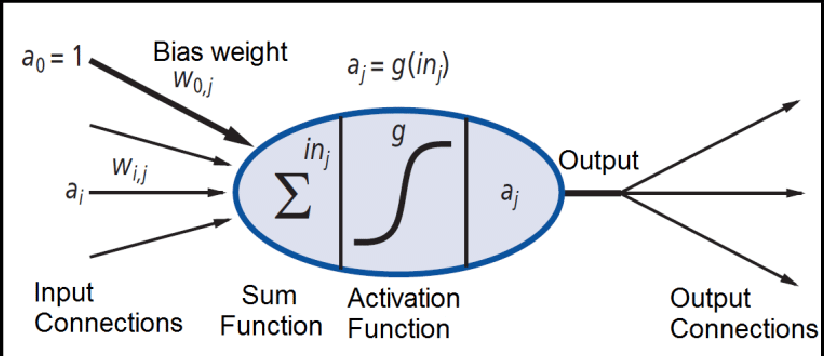
\includegraphics[width=0.75\textwidth]{img/An-artificial-neuron-and-its-various-components-Adapted-from-Norvig-Russel-2013-p.png}
	\caption{Neurone Artificiale}
	\label{Neurone}
\end{figure}
Ogni unità $i$ calcola per prima cosa una somma pesata dei propri input:
\[in_i=\sum_{j=0}^n W_{j,i}\cdot a_j\]
Fatto questo, applica una \textbf{funzione di attivazione} $g$ alla somma per derivare l'output:
\[a_i=g(in_i)=g(\sum_{j=0}^n W_{j,i}\cdot a_j)\]
La funzione di attivazione $g$ è progettata per soddisfare due requisiti:
\begin{itemize}
	\item Prima di tutto desideriamo che l'unità sia attiva (vicina ad 1) quando sono dati i valori giusti di input, altrimenti vogliamo che essa sia inattiva (vicina a -1).
	\item L'attivazione deve essere non lineare.
\end{itemize}Per definire i \textbf{due stati del neurone} si usa l'insieme $\{0, 1\}$ o l'insieme $\{-1, 1\}$ (si ha infatti un \textbf{neurone binario}). La \textbf{funzione di transizione} viene indicata con:
\[s(t+1)=1 \mbox{\textnormal{sse} }\sum w_i\cdot s_i(t)\geq \theta\]
ovvero in un tempo successivo $t+1$ (con $s(t)$ che definisce uno stato al tempo
$t$) ho che il neurone emette il segnale (stato

pari ad 1) sse al tempo precedente $t$ ho avuto una somma pesata, tramite $w_i$,
degli input $a_i(t)$ maggiore della soglia
$\theta$.\\
La funzione di attivazione $g$ può essere rappresentata da diverse funzioni, tra cui:
\begin{itemize}
	\item La funzione Soglia
	\item La funzione Sigmoide/Logistica
\end{itemize}
\begin{figure}[h!]
	\centering
	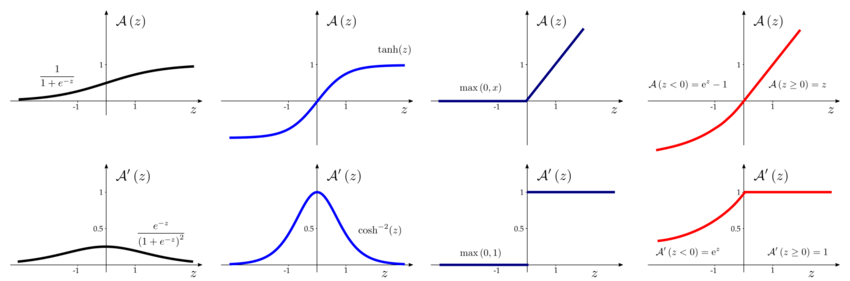
\includegraphics[width=1\textwidth]{img/Some-of-the-most-common-activation-functions-and-their-first-order-gradient-From-left-to.png}
	\caption{Funzioni di Attivazione}
	\label{ActivationFunction}
\end{figure}
L'insieme degli stati, rappresentato in modo binario, comporta che la funzione
di transizione sia una \textbf{funzione soglia}:
\[g(\sum_{j=0}^n W_{j,i}\cdot a_j)=
	\begin{cases}
		1 & \mbox{se } \sum_{j=0}^n W_{j,i}\cdot a_j\geq \theta \\
		0 & \mbox{altrimenti}                                   
	\end{cases}
\]
Questo modello è comunque estremamente semplificato. L'insieme degli stati
potrebbe non essere booleano ma potrebbe essere $\mathbb{R}$, infatti anche
nella biologia il segnale in uscita dai neuroni è graduato e continuo. Si
potrebbe quindi avere una \textbf{funzione logistica o sigmoide}, dove, avendo
come insieme degli stati $\mathbb{R}$ si avrebbe:
\[f(x)=\frac{1}{1+e^{-x}}\,\,\,\,\mbox{  con } \,\,\, x=\sum w_i\cdot a_i\]
Il peso di \textbf{bias} indicato da $W_{0,j}$ determina la soglia effettiva dell'unità e sarebbe uguale a quello che è indicato da $\theta$.
\begin{definizione}
	Se una rete possiede $s_j$ unità nel layer $j$ e $s_{j+1}$ nel layer $j+1$, allora $W$ avrà dimensioni pari a $s_j+1 \times (s_j + 1)$.
\end{definizione}
L'output della rete può essere simboleggiato in diversi modi, solitamente i diversi testi si accordano su una delle seguenti nomenclature: $y, h_\theta(x), h_w(x)$. Quindi non bisogna confondersi qualora in un esempio comparisse $h_\theta(x)$ al posto di $h_w(x)$.
\section{Struttura della rete}
Ci sono due categorie principali di strutture di reti neurali:
\begin{itemize}
	\item Feed-Forward / Alimentata in avanti
	\item Ricorrenti
\end{itemize}
Questo libro si concentrerà sulle strutture \textbf{Feed-Forward}. Esse sono abitualmente organizzare in \textbf{strati}, in modo tale che ogni unità riceva in input solo dalle unità nello strato immediatamente precedente. Oltretutto esse permettono anche la possibilità di avere degli strati nascosti e, di conseguenza, delle unità nascoste. In questa sezione introdurremo due tipologie di reti neurali:
\begin{itemize}
	\item Single Layer: 
	      Nelle reti neurali a \textbf{single layer} un insieme d'input è direttamente mappato su un layer di output. Questa semplice istanziazione di rete è anche chiamata come \textit{percettrone}.
	\item Multi Layer: dove il layer d'input e quello di output sono separati da un gruppo di \textbf{layer nascosti}. 
\end{itemize}
Solitamente nell'\textbf{input layer} i nodi in input vengono descritti da un \textbf{vettore} $X = a_0$.
\subsection{Reti neurali a uno strato alimentate in avanti: il percettrone}
Questa tipologia di architettura possiede un singolo \textbf{input layer} e un \textbf{output layer}. La figura \ref{Percettrone} mostra un esempio della struttura.
\begin{figure}[h]
	\centering
	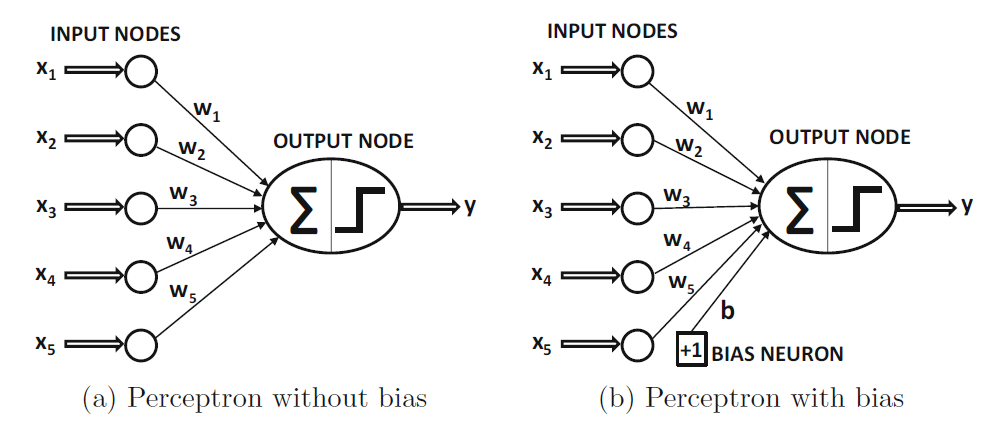
\includegraphics[width=1\textwidth]{img/Capture.PNG}
	\caption{Percettrone}
	\label{Percettrone}
\end{figure}
\begin{definizione}
	Un percettrone è una collezione di neuroni, di cardinalità $M$, a cui viene
	aggiunto un insieme di nodi in input, di cardinalità $N$ (generalmente
	diversa da quella della collezione di neuroni). Generalmente gli input sono
	pesati e con la notazione $w_{ij}$ indichiamo il peso della connessione tra il
	nodo $i$-simo in input e il neurone $j$-simo.\\
	I neuroni sono tra loro completamente indipendenti comportando anche un
	insieme di elementi in output. Nel caso semplice di funzioni di transizione
	binarie l'output sarà quindi un vettore binario contenente all'indice $k$-simo
	1 se il neurone $k$ ha inviato il segnale o 0 altrimenti. \\
	Solitamente coi percettroni si parla di \textit{learning supervisionato}.
\end{definizione}
Sappiamo che un percettrone a \textbf{soglia} restituisce 1 se e solo se la somma pesata dei suoi input (bias incluso) è positiva:
\[\sum_{j=0}^n W_j\cdot x_j > 0\]\,\,\,\mbox{oppure}\,\,\,\[W\cdot x > 0\]
Dal punto di vista geometrico l'equazione $W\cdot x$ rappresenta un 
\textbf{iperpiano} nello spazio d'input (che è una retta in $\mathbb{R}^2$) che separa i possibili
vettori d'input in due classi, a seconda che formino con $W$ un angolo acuto o
ottuso. Quindi il percettrone restituisce $1$ se e solo se l'input si trova da una parte specifica rispetto a tale iperpiano. Per questa ragione, il percettrone a soglia è chiamato anche \textbf{separatore lineare}. Difatti esso può rappresentare \textbf{funzioni linearmente separabili} (fig. \ref{SeparatoreLineare}).\\
\begin{figure}[h!]
	\centering
	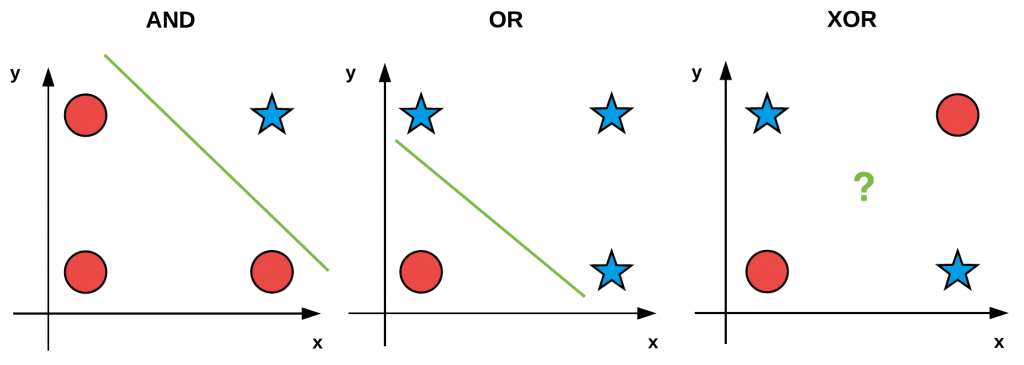
\includegraphics[width=1\textwidth]{bitwise_datasets-1024x365.png}
	\caption{Separatore Lineare}
	\label{SeparatoreLineare}
\end{figure}
È chiaro quindi che i \textbf{percettroni a soglia possono rappresentare solo funzioni linearmente separabili}. D'altro Canto esiste un semplice algoritmo di apprendimento capace di adattare un percettrone a soglia a qualsiasi insieme di addestramento linearmente separabile.
\subsubsection{Algoritmo del percettrone e Discesa del Gradiente}
Fino a ora il singolo neurone rappresentava un singolo iperpiano che veniva ``spostato'' per dividere le istanze positive e quelle negative. Ora introduciamo che a ogni passo di aggiornamento si aggiornano i pesi e se, mano a mano che cambio i pesi, misuro l'errore sul dataset del mio sistema. Si può quindi far ``scendere'' questo errore e ci si augura che ci sia una costante di discesa dell'errore. L'idea di questo algoritmo è di calibrare i pesi nella rete in modo da minimizzare una qualche misura di errore sull'insieme di training. Quindi L'apprendimento è formulato come una ricerca di ottimizzazione nello \textbf{spazio dei pesi}. La misura di errore è la \textbf{somma dei quadrati degli errori}.
Il quadrato dell'errore per un singolo esempio di training con input $x$ e output $y$ si scrive:
\[E=\frac{1}{2}(y-h_w(x))^2\]\mbox{Dove $h_w(x)$ è l'output del percettrone per l'esempio.}

Possiamo usare il \textbf{metodo della discesa di gradiente} per ridurre il quadrato dell'errore calcolando la derivata parziale di $E$ rispetto a ogni peso. Nell'algoritmo a discesa del gradiente, in cui vogliamo \textbf{ridurre} E, aggiorniamo i pesi come segue:
\[w_{ij}\gets w_{ij}+\eta\cdot(y-h_w(x))\times a_i\]
Si calcola il gradiente della curva degli errori e si punta a essere sempre in ``discesa'' lungo la curva dell'errore, aggiustando in modo opportuno i pesi. Viene anche introdotto il \textbf{learning rate (\textit{tasso di apprendimento})} $\eta$, utile per stabilire la velocità di apprendimento della rete. In pratica $\eta$ decide quanto cambiare il peso (e se si vuole trascurare il parametro basta porre $\eta =1$). L'uso di tale parametro migliora la stabilità della \textit{rete neurale} che non avrà cambi di peso eccessivi, anche se
questo comporta tempi di apprendimento più estesi. Tipicamente si ha che:
\[0.1\leq\eta\leq 0.4\]
Si noti che se l'errore $y-h_w(x)$ è positivo allora $y>h_w(x)$ quindi l'output della rete dev'essere troppo piccolo e quindi i pesi aumentano per gli input positivi e diminuiscono per quelli negativi. Quando l'errore è negativo avviene l'opposto. Gli esempi di addestramento vengono fatti passare attraverso la rete uno per volta, modificando leggermente i pesi a ogni iterazione per ridurre l'errore. Ogni ciclo attraverso tutto gli esempi prende il nome di \textbf{epoca}. Le epoche sono tipicamente ripetute fino a quando non viene soddisfatto qualche criterio di terminazione. Si ha che a ogni iterazione ci si aspetta un miglioramento della \textit{rete neurale} (e questo miglioramento è dimostrabile). Viene imposto
quindi un limite $T$ d'iterazioni entro le quali interrompere l'apprendimento anche se non si è arrivati al risultato
corretto.
% \begin{algorithm}[h] % TODO: modify
% 	\begin{algorithmic}
% 		\Function{grad}{}
% 		\State \textit{inizializzo ogni $\Delta w_i$ a $0$}
% 		\For {\textit{ogni input $\langle( x_1, \ldots x_n), t\rangle$}}
% 		\State \textit{invio l'input $( x_1, \ldots x_n)$ all'unità lineare e
% 		calcola l'output $y$} 
% 		\State \textit{aggiorno la variazione dei pesi:}
% 		\[\Delta w_i=\Delta w_i+\eta\cdot (t-y)\cdot x_i\]
% 		\EndFor
% 		\State \textit{aggiorno i pesi:}
% 		\[w_i=w_i+\Delta w_i\]
% 		\EndFunction
% 	\end{algorithmic}
% 	\caption{Algoritmo di discesa lungo il gradiente}
% \end{algorithm}
% Abbiamo una \textbf{modalità Batch}, quindi computazionalmente costosa:
% \[w=w-\eta\cdot\nabla E_D[W]\]
% Si può avere una \textbf{modalità incrementale}:
% \[w=w-\eta\cdot\nabla E_d[W]\]
% calcolata sui singoli esempi $d$:
% \[E_d[w]=\frac{1}{2}(t_d-y_d)^2\]
% La discesa lungo il gradiente incrementale può approssimare la discesa lungo
% il gradiente Batch arbitrariamente se $\eta$ è abbastanza piccolo.\\
% Rispetto a quanto visto per il percettrone la discesa lungo il gradiente
% converge all'ipotesi con il minimo errore quadratico se  $\eta$ è abbastanza
% basso, anche per dati di training molto rumorosi.

% \[\Delta w_{ik}=-(y_k-t_k)\times a_i\]
% In questo discorso bisogna inserire anche la soglia, importante per input
% specifici (basti pensare a un input pari a 0 che annullerebbe ogni cambio di
% peso secondo la formula precedente). Per ora trascureremo tali casi anche se una
% semplice soluzione per un caso limite come quello di avere solo input nulli, è
% quella di aggiungere un \textbf{nodo bias}, di valore $-1$, collegato ai neuroni
% con peso nullo.\\


\subsubsection{Approfondimento sul Percettrone}
Vediamo due teoremi utili per lo studio dell'apprendimento del percettrone su due classi $A$ e $B$, banalmente rappresentanti, nella nostra situazione binaria e semplificata, il caso in cui si abbia il neurone che emette il segnale (valore 1 in output) o altrimenti (valore 0 in output). Nel nostro caso le classi sono discriminabili.
\begin{definizione}[definizione di convergenza]
	Comunque si scelgano i pesi iniziali, se le classi A e B sono discriminabili,
	la procedura di apprendimento termina dopo un numero finito di passi
\end{definizione}
\begin{definizione}[definizione di Minsky e Papert]
	La classe delle forme discriminabili da un percettrone semplice è
	limitata alle forme linearmente separabili
\end{definizione}
In base a questo si distinguerà in:
\begin{itemize}
	\item \textbf{addestramento separabile}, quando si ha un iperpiano che separa
	      le istanze positive e negative
	\item \textbf{addestramento non separabile}
\end{itemize}
Per capire il discorso della \textbf{separabilità} vediamo un esempio.
\begin{esempio}
	Vediamo un esempio che tratta l'addizione binaria, ovvero l'\textit{or
	esclusivo}.
	Le possibili istanze sono rappresentate nel piano:
	\begin{figure}[H]
		\centering
		\psscalebox{1.0 1.0} % Change this value to rescale the drawing.
		{
			\begin{pspicture}(0,-1.9534792)(5.906958, 1.9534792)
				\psline[linecolor=black, linewidth=0.04,
					arrowsize=0.05291667cm 2.0, arrowlength=1.4
				, arrowinset=0.0]{->}(2.4,-1.9534792)(2.4, 1.6465209)(2.4, 2.046521)
				\psline[linecolor=black, linewidth=0.04,
					arrowsize=0.05291667cm 2.0, arrowlength=1.4,
				arrowinset=0.0]{->}(1.6,-1.1534791)(6.0,-1.1534791)
				\psdots[linecolor=black, dotsize=0.4](2.4, 0.84652084)
				\psdots[linecolor=black, dotsize=0.4](4.4, 0.84652084)
				\psdots[linecolor=black, dotsize=0.4](4.4,-1.1534791)
				\psdots[linecolor=black, dotsize=0.4](2.4,-1.1534791)
				\rput[bl](0.4, 0.68652084){$0\oplus 1=1$}
				\rput[bl](0.4,-0.7534792){$0\oplus  1=0$}
				\rput[bl](3.4,-0.7534792){$1\oplus 0=1$}
				\rput[bl](3.4, 1.2465209){$1\oplus 1=0$}
			\end{pspicture}
		}
	\end{figure}
	Ho quindi che nessuna retta potrà separare tutti i punti e
	quindi i punti a valore 1 \textbf{non sono linearmente separabili} da quelli a
	valore 0.\\
	Si vorrebbe cercare un neurone binario a soglia tale che:
	\[x\oplus y=1\iff \alpha\cdot x+\beta\cdot y\geq \lambda\]
	Tale neurone si rappresenterebbe con:
	\begin{figure}[H] 
		\centering
		\psscalebox{1.0 1.0} % Change this value to rescale the drawing.
		{
			\begin{pspicture}(0,-1.9534792)(5.906958, 1.9534792)
				\pscircle[linecolor=black, linewidth=0.04,
				dimen=outer](3.2, 0.24245118){0.8}
				\psline[linecolor=black, linewidth=0.04,
					arrowsize=0.05291667cm 2.0, arrowlength=1.4,
				arrowinset=0.0]{->}(0.4, 0.64245117)(2.4, 0.64245117)
				\psline[linecolor=black, linewidth=0.04, arrowsize=0.05291667cm 2.0,
				arrowlength=1.4, arrowinset=0.0]{->}(0.4,-0.15754883)(2.4,-0.15754883)
				\psline[linecolor=black, linewidth=0.04, arrowsize=0.05291667cm 2.0,
				arrowlength=1.4, arrowinset=0.0]{->}(4.0, 0.24245118)(6.0, 0.24245118)
				\rput[bl](0.0, 0.56245117){$x$}
				\rput[bl](0.0,-0.32754883){$y$}
				\rput[bl](1.2, 0.8245117){$\alpha$}
				\rput[bl](1.2, 0.024245118){$\beta$}
				\rput[bl](3.07, 0.115754886){$\lambda$}
				\rput[bl](6.2, 0.0824245118){$x\oplus y$}
			\end{pspicture}
		}
	\end{figure}
	ma appunto tale neurone non può esistere in quanto non potrei mai separare
	i punti a valori 1 e quelli a valore 0 con una retta. Posso infatti separare o
	singoli punti o coppie di punti a valore opposto o triple di punti ma non
	potrò mai avere separati insiemi con tutti gli 0 e tutti gli 1.
\end{esempio}
\begin{definizione}
	Se l'insieme degli input estesi è partito in due classi linearmente separabili
	allora:
	\[\exists\,\, W\mbox{t.c }
		\begin{cases}
			1 & \mbox{se } \sum w_i\cdot a_i \geq 0 \\
			0 & \mbox{se } \sum w_i\cdot a_i < 0    
		\end{cases}
	\]
	con $W$ \textbf{vettore dei pesi}.
\end{definizione}
Vediamo quindi l'algoritmo di learning per un percettrone, data la
\textbf{funzione di transizione} per un input di cardinalità $m$ e $n$ neuroni:
\[
	y_j=g\left(\sum_{i=0}^m w_{ij}\cdot a_i \right)=
	\begin{cases}
		1 & \mbox{se } \sum_{i=0}^m w_{ij}\cdot a_i > 0    \\
		0 & \mbox{se } \sum_{i=0}^m w_{ij}\cdot a_i \leq 0 
	\end{cases}
\]
Vediamo quindi l'algoritmo di apprendimento del percettrone:
\begin{algorithm}[H]
	\begin{algorithmic}
		\Function{perceptron-learning}{}
		\State \textit{\color{gray}{\# Inizializzazione}}
		\State \textit{si imposta tutti i pesi $w_{ij}$ a valori casuali piccoli
		(anche negativi)}
		\State \textit{\color{gray}{\# Training}}
		\For {\textit{$T$ iterazioni \textbf{o} fino a che tutti gli output non sono
		corretti}}
		\For {\textit{ogni vettore input}}
		\State \small{\color{gray}{\textit{\# calcolo l'attivazione di ogni neurone
		$j$ }}}
		\State \small{\color{gray}{\textit{\# tramite la funzione di transizione
		$g$:}}} 
		\State $y_j=g\left(\sum_{i=0}^m w_{ij}\cdot a_i \right)=
		\begin{cases} 1
			  & \mbox{se } \sum_{i=0}^m w_{ij}\cdot a_i > 0 \\ 0 &\mbox{se }
			\sum_{i=0}^m w_{ij}\cdot a_i \leq 0
		\end{cases}$ 
		\State {\textit{\color{gray}\# aggiorno ogni peso individualmente}}
		\State {\textit{\color{gray}\# nella prossima iterazione avrò nuovi pesi}}
		\State $w_{ij}\gets w_{ij}-\eta\cdot(y_j-t_j)\times a_i$
		\EndFor
		\EndFor
		\State {\textit{\color{gray}\# Recall}}
		\State \small{\color{gray}{\textit{\# ricalcolo l'attivazione di ogni
		neurone $j$ tramite:}}} 
		\State $y_j=g\left(\sum_{i=0}^m w_{ij}\cdot a_i \right)=
		\begin{cases} 1
			  & \mbox{se } w_{ij}\cdot a_i > 0 \\ 0 &\mbox{se }
			w_{ij}\cdot a_i \leq 0
		\end{cases}$
		\EndFunction
	\end{algorithmic}
	\caption{Algoritmo di learning del percettrone}
\end{algorithm}
La complessità dell'algoritmo è $O(Tnm)$.\\
Si può dimostrare, tramite il \textbf{definizione della convergenza del percettrone}
che dopo $\beta$ modifiche di peso il percettrone classifica 
correttamente ogni input anche se tale $\beta$ non è il reale numero di stadi e
dipende dall'output.\\
L'algoritmo di apprendimento del percettrone quindi \textit{converge} alla
classificazione corretta quindi se:
\begin{itemize}
	\item i dati di training sono linearmente separabili
	\item $\eta$ è abbastanza piccolo
\end{itemize}
\begin{definizione}
	Se l'insieme degli input estesi è partito in due classi linearmente separabili
	$A$ e $B$ allora é possibile trovare un vettore di pesi $w$ tale che:
	\[
		\begin{cases}
			\langle w, x\rangle\geq 0 & \mbox{se }x\in A \\
			\langle w, x\rangle < 0   & \mbox{se }x\in B 
		\end{cases}
	\]
	Quindi:
	\begin{itemize}
		\item si parte con $w$ arbitrario
		\item si classifica un punto $x$:
		      \begin{itemize}
		      	\item se la risposta è corretta si ha $w'\gets w$
		      	\item se la risposta è errata:
		      	      \[
		      	      	\begin{cases}
		      	      		w'\gets w+x & \mbox{se }x\in A \\
		      	      		w'\gets w-x & \mbox{se }x\in B \\
		      	      	\end{cases}
		      	      \]
		      \end{itemize}
	\end{itemize}
	
\end{definizione}
\begin{proof}
	Vediamo la prova della correttezza del definizione.\\
	Se si ha $x\in A$ allora si ha $\langle w, x\rangle<0$ infatti, poiché:
	\[\langle x, x\rangle\geq 0\]
	si ha che:
	\[\langle w', x\rangle=\langle (w+x), x\rangle=\langle w, x\rangle+\langle x,
		x\rangle>\langle w, x\rangle\]
		Quindi $w'$ classifica $x$ in modo più corretto di $w$ anche se altri input
		possono essere classificati "meno correttamente".
		\end{proof}
		\begin{proof}
			Passiamo ora alla convergenza.\\
			Consideriamo quindi $A'=A\cup B'$ con:
			\[B'=\{-x|\, x\in B\}\]
			e cerchiamo un $v$ tale che:
			\[\langle v, x\rangle\geq 0,\,\,\forall\, x\in A'\]
			Si hanno quindi:
			\begin{itemize}
				\item la \textbf{sequenza di addestramento} $\{x_i\}_{i\in N}$ dove $x_i\in
				      A'$ e quindi la sequenza ontiene infiniti elementi sia di $A$ che di $B'$
				\item la \textbf{sequenza di pesi} $\{w_i\}_{i\in N}$ dove si parte
				      arbitrariamente con $w_0=0$ e si procede con:
				      \[
				      	\begin{cases}
				      		w_{k+1}\gets w_k     & \mbox{se }\langle w_k, x_k\rangle\geq 0 \\
				      		w_{k+1}\gets w_k+x_k & \mbox{altrimenti}                       
				      	\end{cases}
				      \]
			\end{itemize}
			Si hanno quindi:
			\begin{itemize}
				\item la \textbf{sequenza di pesi modificata} $\{v_i\}_{i\in N}$ 
				\item la \textbf{sottosequenza di training corrispondente} $\{v_i\}_{i\in N}$ 
			\end{itemize}
			Di modo che le coppie $(v_i, t_i)$ corrispondano ai $w_j$ tali per cui $w_j\neq
			w_{j+1}$.\\
			Ad esempio per:
			\[w_0\neq w_1=w_2=w_3\neq w_4=w_5=w_6\neq w_7\neq w_8\cdots\]
			avremo:
			\begin{itemize}
				\item $(v_0, t_0)$ associati a $w_0$
				\item $(v_1, t_1)$ associati a $w_3$
				\item $(v_2, t_2)$ associati a $w_6$
				\item $(v_3, t_3)$ associati a $w_7$
			\end{itemize}
			Avendo:
			\[\langle v_i, t_i\rangle<0\,\,\,\forall i\]
			e avendo:
			\[v_{i+1}=v_i+t_i=v_{i-1}+t_{i-1}+y_i=\sum_{k=0}^i t_i\]
			e quindi la sequenza $\{v_i\}$ è \textbf{finita}.
		\end{proof}
		\begin{proof}
			Uniamo matematicamente in una sola dimostrazione.\\
			Sia $w$ una qualsiasi soluzioni che sappiamo esistere per ipotesi. Si ha che:
			\[\langle v, x\rangle\geq 0,\,\,\forall\, x\in A'\]
			Pongo quindi:
			\[\alpha=\min(\langle x, w\rangle,\,\,\forall\, x\in A')\]
			sapendo che:
			\[v_{i+1}=v_i+t_i=v_{i-1}+t_{i-1}+y_i=\sum_{k=0}^it_i\]
			ho che:
			\[\langle v_{i+1}, w\rangle=\langle \left(\sum_{k=0}^i t_k \right),
				w\rangle\geq (i+1)\cdot\alpha\]
				ma usando il definizione di \textbf{Cauchy-Schwarz} si ha che:
				\[(\langle v_{i+1}, w\rangle)^2\leq \langle |v_{i+1}|^2,|w|^2\rangle\]
				ottenendo che:
				\[|v_{i+1}|^2\geq \frac{(i+1)^2\cdot \alpha^2}{|w|^2}\]
				Pongo quindi:
				\[M=\max\{|x|^2|,\, x\in A'\}\]
				si ha che, avendo $\langle v_{1}, t_i\rangle<0$:
				\[|v_{i+1}|^2=|v_i+t_i|^2=|v_i|^2+2\cdot\langle v_{i}, t_i\rangle+|t_i|^2\leq
					|v_i|^2+|t_i|^2\]
					Si ha, di conseguenza:
					\[|v_{i+1}|^2\leq \sum_{k=1}^i |t_i|^2\leq i\cdot M\]
					Unendo quest'ultima con $|v_{i+1}|^2\geq \frac{(i+1)^2\cdot \alpha^2}{|w|^2}$
					si ha che:
					\[f(i)=\frac{j^2\cdot \alpha^2}{|w|^2}\leq |v_{i+1}|^2\leq i\cdot M=g(i)\]
					avendo che $\frac{j^2\cdot \alpha^2}{|w|^2}$ è quadratico in $i$ e $ i\cdot M$
					lineare in $i$.\\
					Si ottiene quindi che:
					\[i\leq\frac{M\cdot |w|^2}{\alpha^2}=\beta\]
					Quindi dopo $\beta$ modifiche di peso il percettrone classifica correttamente
					ogni input.
					\end{proof}
					\subsubsection{Esercitazione sul percettrone}
					Il percettrone si basa su un'unica unità di calcolo e tramite una funzione
					soglia valorizza l'uscita in modo da farle assumere un valore booleano in
					$\{-1, 1\}$.\\
					Si hanno vari pesi $w_i$ che scalano l'ingresso e, insieme agli input $x_i$
					(compreso l'input bias),
					formano il \textbf{potenziale di attivazione}:
					\[\sum_{i=0}^nw_ix_i=\langle \overline{w}, \overline{x}\rangle\]
					che verrà poi fatto passare per la funzione
					soglia. Se il potenziale è positivo si avrà uno in uscita, se negativo o nullo
					-1:
					\[output=
						\begin{cases}
							1  & \mbox{se } \sum w_i\cdot x_i > 0    \\
							-1 & \mbox{se } \sum w_i\cdot x_i \leq 0 
						\end{cases}
					\]
					In letteratura si hanno modelli dove il potenziale nullo comporta una terza
					uscita pari a 0.\\
					Il percettrone basa il suo algoritmo di training su un ciclo che aggiorna di
					volta in volta i pesi intermedi.
					Per il percettrone si ha quindi una funzione di aggregazione del tipo:
					\[z=b+\sum_{i=1}^nw_ix_i\]
					(con $b$ valore del nodo bias)\\
					che viene passata alla funzione soglia:
					\[f(z)=\hat{y}\]
					calcolando l'output:
					\[\hat{y}\in\{-1, 1\}\]
					Per aggiornare i pesi si calcola l'errore (la differenza tra il valore calcolato
					$\hat{y}$ e la label associata all'esempio in analisi $y$):
					\[error=y-\hat{y}\]
					calcola la correzione del peso, tramite la fattorizzazione dei pesi:
					\[\Delta w=\eta(error)x_k\]
					e aggiornando poi i pesi:
					\[w_{k+1}=w_k+\Delta w_k\]
					Nel caso di Adaline si ha una struttura in realtà simile ma utilizza una
					valutazione nel continuo degli errori, ad esempio tramite una certa funzione
					lineare. La funzione prende prende in input il potenziale di attivazione e la
					cui uscita viene valutata per il calcolo dell'errore $\delta$ tramite la
					\textbf{$\delta$ rule} ($\delta$ che ha valore continuo e non booleano). Si ha
					comunque una funzione di uscita a soglia che funziona come per il percettrone
					standard, se positivo il risultato restituisce 1 altrimenti -1.\\
					Per Adaline si ha quindi una funzione di aggregazione del tipo:
					\[\hat{y}=b+\sum_{i=1}^nw_ix_i\]
					(con $b$ valore del nodo bias)\\
					che viene passata alla funzione soglia:
					\[f(\hat{y})\]
					per produrre l'uscita booleana (uguale al percettrone):
					\[\hat{y}'\in\{-1, 1\}\]
					per l'update dell'errore, a partire dalla funzione di aggregazione, si procede
					circa come per il percettrone standard, avendo però un errore quadratico:
					\[error=(y-\hat{y})^2\]
					e avendo poi l'update tramite:
					\[w_{k+1}=w_k-\eta(2error_k)x_k\]
					Riassumendo abbiamo l'algoritmo del percettrone che, per ogni esempio $\langle
					x, t\rangle$ con $t$ label, esegue:
					\begin{enumerate}
						\item $y=step(f(x))$ (con step che da il booleano a seconda del segno)
						\item $w=w+\eta(t-y)x$
					\end{enumerate}
					Si ha che:
					\begin{itemize}
						\item se l'output matcha il target allora $t-y$ è nullo e non si aggiornano i
						      pesi
						\item se l'output è 1 ma il target è 0 l'input, scalato con learning rate
						      $\eta$, viene sottratto dal vettore dei pesi
						\item se l'output è 0 ma il target è 1 l'input, scalato con learning rate
						      $\eta$, viene aggiunto al vettore dei pesi
					\end{itemize}
					Riassumendo abbiamo l'algoritmo del Adaline che, per ogni esempio $\langle
					x, t\rangle$ con $t$ label, esegue:
					\begin{enumerate}
						\item $y=f(x)$
						\item $w=w+\eta(t-y)x$
					\end{enumerate}
					Si ha che questo equivale la regola del \textit{gradient descent} della
					regressione lineare (con errore quadratico), infatti la derivata di $(y-t)^2$ è
					$2(z-t)$. Il fattore costante 2 può essere omesso dato che si usa il learning
					rate per rimodulare quanto aggiornare i pesi.\\
					Ovviamente entrambi possono studiare solo set di punti separabili linearmente,
					usando iperpiani e non rette se saliamo di grado su $\mathbb{R}$, per separare i
					punti.
					\begin{esercizio}
						Prendiamo il seguente training set con $t(x)$ che ci fornisce la label:
						\begin{table}[H]
							\centering
							\begin{tabular}{c||c|c|c}
								      & $x$ & $y$  & $t(x)$ \\
								\hline
								\hline
								$x_1$ & 1   & 1    & 1      \\
								$x_2$ & 2   & -2   & -1     \\
								$x_3$ & -1  & -1.5 & 1      \\
								$x_4$ & 1   & -2   & -1     \\
								$x_5$ & -2  & -1   & 1      \\
							\end{tabular}
						\end{table}
						graficamente possiamo rappresentare tali punti (in blu con target $+1$ e rosso
						per target $-1$, notando che sono linearmente separabili):
						\begin{figure}[H]
							\centering
							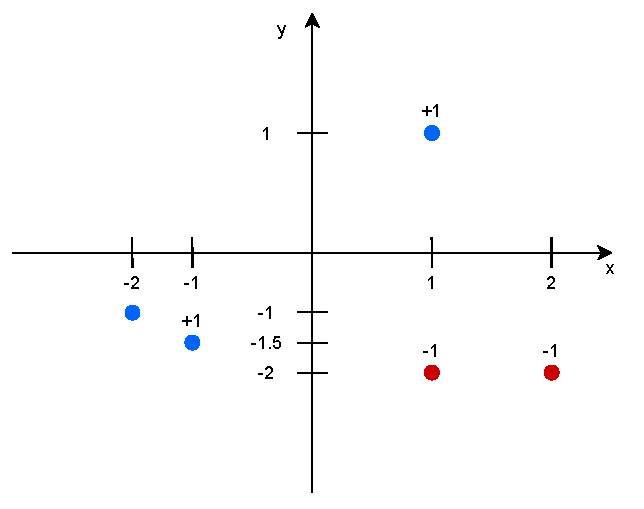
\includegraphics[scale = 0.8]{img/per1.pdf}
						\end{figure}
						Usiamo quindi l'algoritmo del percettrone e studiamo come si aggiornano i
						pesi. Si impone $\eta=0.2$ e nodo bias di valore $b=1$ e peso $w_0$,
						arbitrariamente inizializzato a 0.\\ 
						Partiamo con il primo esempio. Si hanno:
						\begin{itemize}
							\item $x_1=(1, 1)$
							\item $t(x_1)=1$
						\end{itemize}
						da ciò si ricava che l'input del percettrone, il suo segnale d'ingresso, altro
						non è che, considerando il nodo bias:
						\[\overline{x}=(b, x_1)=(1, 1, 1)\]
						Arbitrariamente inizializziamo i pesi a (avendo già detto che il bias ha peso
						0):
						\[\overline{w}=(0, 1, 0.5)\]
						Faccio quindi il prodotto scalare tra il vettore input e il vettore peso:
						\[\langle \overline{w}, \overline{x}\rangle=
							\left(\begin{matrix}
							0 & 1 & 0.5
							\end{matrix}\right)
							\left(
							\begin{matrix}
								1 \\
								1 \\
								1 \\
							\end{matrix}
							\right)= 0 + 1 + 0.5 = 1.5
						\]
						Si ha quindi $\langle \overline{w}, \overline{x}\rangle > 0$ e quindi:
						\[sign(\langle \overline{w}, \overline{x}\rangle)=+1\]
						e avendo che, ricordando $t(x_1)=+1$:
						\[sign(\langle \overline{w}, \overline{x}\rangle)=t(x_1)\]
						i pesi $\overline{w}$ non devono essere aggiornati.\\
						Si passa al secondo esempio.\\
						Si ha (senza dover rispiegare gli step metto tutto nella stessa lista):
						\begin{itemize}
							\item $x_2=(2,-2)$
							\item $t(x_2)=-1$
							\item $\overline{x}=(1, 2,-2)$
							\item $\overline{w}=(0, 1, 0.5)$
						\end{itemize}
						calcolo:
						\[\langle \overline{w}, \overline{x}\rangle=
							\left(\begin{matrix}
							0 & 1 & 0.5
							\end{matrix}\right)
							\left(
							\begin{matrix}
								1  \\
								2  \\
								-2 \\
							\end{matrix}
							\right)= 0 + 2 - 1 = 1
						\]
						Si ha quindi $\langle \overline{w}, \overline{x}\rangle > 0$ e quindi:
						\[sign(\langle \overline{w}, \overline{x}\rangle)=+1\]
						e avendo che, ricordando $t(x_2)=-1$:
						\[sign(\langle \overline{w}, \overline{x}\rangle)\neq t(x_2)\]
						Bisogna procedere all'update dei pesi, che ricordiamo essere:
						\[\overline{w}_{new}=\overline{w}_{old}+\eta(y-\hat{y})\overline{x}\]
						\newpage
						si ha quindi, avendo $\hat{y}=1, y=-1$ e quindi $y-\hat{y}=-2$:
						\begin{itemize}
							\item
							      $\overline{w}_{new}[0]=\overline{w}_{old}[0]+0.2\cdot (-2)\cdot
							      x[0]=0+0.2\cdot(-2)\cdot 1=-0.4$ 
							\item
							      $\overline{w}_{new}[1]=\overline{w}_{old}[1]+0.2\cdot (-2)\cdot
							      x[1]=1+0.2\cdot(-2)\cdot 2=0.2$ 
							\item
							      $\overline{w}_{new}[2]=\overline{w}_{old}[2]+0.2\cdot (-2)\cdot x[2]=0.5+0.2
							      \cdot(-2)\cdot(-2)=1.3$    
						\end{itemize}
						ottenendo quindi come nuovo vettore dei pesi:
						\[\overline{w}=(-0.4, 0.2, 1.3)\]
						Passo quindi al terzo esempio:
						\begin{itemize}
							\item $x_3=(-1,-1.5)$
							\item $t(x_3)=-1$
							\item $\overline{x}=(1,-1,-1.5)$
							\item $\overline{w}=(-0.4, 0.2, 1.3)$
						\end{itemize}
						calcolo:
						\[\langle \overline{w}, \overline{x}\rangle=
							\left(\begin{matrix}
							-0.4 & 0.2 & 1.3
							\end{matrix}\right)
							\left(
							\begin{matrix}
								1   \\
								-1  \\
								1.5 \\
							\end{matrix}
							\right)= -0.4-0.2-1.95 = -2.55
						\]
						Si ha quindi $\langle \overline{w}, \overline{x}\rangle \leq 0$ e quindi:
						\[sign(\langle \overline{w}, \overline{x}\rangle)=-1\]
						e avendo che, ricordando $t(x_3)=+1$:
						\[sign(\langle \overline{w}, \overline{x}\rangle)\neq t(x_3)\]
						Bisogna procedere all'update dei pesi, avendo $\hat{y}=-1, y=1$ e quindi
						$y-\hat{y}=2$:
						\begin{itemize}
							\item
							      $\overline{w}_{new}[0]=\overline{w}_{old}[0]+0.2\cdot 2\cdot
							      x[0]=-0.4+0.2\cdot 2\cdot 1=0$ 
							\item
							      $\overline{w}_{new}[1]=\overline{w}_{old}[1]+0.2\cdot 2\cdot
							      x[1]=0.2+0.2\cdot 2\cdot (-1)=-0.2$ 
							\item
							      $\overline{w}_{new}[2]=\overline{w}_{old}[2]+0.2\cdot 2\cdot x[2]=1.3+0.2
							      \cdot 2\cdot(-1.5)=0.7$    
						\end{itemize}
						ottenendo quindi come nuovo vettore dei pesi:
						\[\overline{w}=(0, -0.2, 0.7)\]
						Passo quindi al quarto esempio:
						\begin{itemize}
							\item $x_4=(1,-2)$
							\item $t(x_4)=-1$
							\item $\overline{x}=(1, 1,-2)$
							\item $\overline{w}=(0, -0.2, 0.7)$
						\end{itemize}
						calcolo:
						\[\langle \overline{w}, \overline{x}\rangle=
							\left(\begin{matrix}
							0 & -0.2 & 0.7
							\end{matrix}\right)
							\left(
							\begin{matrix}
								1  \\
								1  \\
								-2 \\
							\end{matrix}
							\right)= 0-0.2-1.4 = -1.6
						\]
						Si ha quindi $\langle \overline{w}, \overline{x}\rangle \leq 0$ e quindi:
						\[sign(\langle \overline{w}, \overline{x}\rangle)=-1\]
						e avendo che, ricordando $t(x_4)=-1$:
						\[sign(\langle \overline{w}, \overline{x}\rangle)= t(x_4)\]
						E quindi non devo aggiornare i pesi.\\
						Passo quindi al quinto esempio:
						\begin{itemize}
							\item $x_5=(-2,-1)$
							\item $t(x_5)=1$
							\item $\overline{x}=(1,-2,-1)$
							\item $\overline{w}=(0, -0.2, 0.7)$
						\end{itemize}
						calcolo:
						\[\langle \overline{w}, \overline{x}\rangle=
							\left(\begin{matrix}
							0 & -0.2 & 0.7
							\end{matrix}\right)
							\left(
							\begin{matrix}
								1  \\
								-2 \\
								-1 \\
							\end{matrix}
							\right)= 0+0.4-0.7 = -0.3
						\]
						Si ha quindi $\langle \overline{w}, \overline{x}\rangle \leq 0$ e quindi:
						\[sign(\langle \overline{w}, \overline{x}\rangle)=-1\]
						e avendo che, ricordando $t(x_5)=+1$:
						\[sign(\langle \overline{w}, \overline{x}\rangle)\neq t(x_5)\]
						Bisogna procedere all'update dei pesi, avendo $\hat{y}=-1, y=1$ e quindi
						$y-\hat{y}=2$:
						\begin{itemize}
							\item
							      $\overline{w}_{new}[0]=\overline{w}_{old}[0]+0.2\cdot 2\cdot
							      x[0]=0+0.2\cdot 2\cdot 1=0.4$ 
							\item
							      $\overline{w}_{new}[1]=\overline{w}_{old}[1]+0.2\cdot 2\cdot
							      x[1]=0.2+0.2\cdot 2\cdot (-2)=-1$ 
							\item
							      $\overline{w}_{new}[2]=\overline{w}_{old}[2]+0.2\cdot 2\cdot x[2]=0.7+0.2
							      \cdot 2\cdot(-1)=0.3$    
						\end{itemize}
						ottenendo quindi come nuovo vettore dei pesi:
						\[\overline{w}=(0.4, -1, 0.3)\]
						che, avendo terminato l'esercizio, è il vettore pesi finale usato
						dall'algoritmo. 
					\end{esercizio}
					\subsection{Reti multistrato}
					\textbf{Le formule più complesse sono solo di bellezza.}\\
					\noindent
					Passiamo quindi dal percettrone a una rete a due strati, cambiando quindi la
					gestione dei pesi.\\
					Devo avere sempre un gradiente dei pesi, che ora avranno doppio indice per
					indicare anche l'unità di riferimento, che scende:
					\[\frac{\partial E}{\partial w_{ij}}=\frac{\partial E}{\partial y_{j}}\cdot
						\frac{\partial y_j}{\partial w_{ij}}=-(t_j-y_j)\cdot \frac{\partial
							y_j}{\partial w_{ij}}=-\delta_j\cdot\frac{\partial \sum_i w_{ij}\cdot
							x_j}{\partial w_{ij}}=-\delta_j\cdot x_i\]
						Si ha quindi:
						\[\Delta w_{ij}=\eta\cdot \delta_j\cdot x_i\]
						detta \textbf{regola delta}, che è l'evoluzione di quanto detto per il
						percettrone in merito alla variazione dei pesi.\\
						Si ha che la convergenza a un minimo globale é garantita per funzioni di
						attivazione lineari senza unità nascoste e per dati consistenti.\\
						Si introduce una nuova funzione di attivazione, detta \textbf{sigmoide}, che
						comporta l'\textbf{unità sigmoide}. La funzione sigmoide è:
						\[y=\sigma(net)=\frac{1}{1+e^{-net}}\]
						Tale funzione è derivabile, infatti:
						\[\dd \sigma(x)=\sigma(x)\cdot (1-\sigma(x))\]
						riprendendo la figura \ref{fig:bin} si ha quindi in primis l'aggiunta del nodo
						bias e poi il cambio della funzione a scalino con il \textbf{sigmoide}. L'output
						invece non sarà più binario ma un certo $y$.\\
						Si hanno quindi in primis le \textbf{reti multistrato feedforward} con le
						seguenti caratteristiche:
						\begin{itemize}
							\item si hanno strati intermedi tra input e output
							\item si hanno connessioni da strati di livello basso a strati di livello
							      alto, solitamente mono direzionali
							\item non si hanno all'interno di uno stesso strato
							\item il neurone ha uno stato booleano $x\in\{0, 1\}$
							\item si ha la seguente funzione di transizione:
							      \[x_k=\sigma\left(\sum_{j}w_{jk}\cdot x_j\right)\]
							      con $x_j$ che può essere in alcuni
							      casi un input istanza e in altri lo stato di altri neuroni, a seconda
							      dell'altezza del livello in cui mi trovo
							\item per ogni configurazione $x$ del primo strato (ingresso), la rete calcola
							      una configurazione $y$ dell'ultimo strato (uscita). Normalmente avremo uno
							      strato nascosto più grande (poco) di quello d'uscita (anche se non si ha una
							      regola per dimensionare lo strato nascosto). Raramente useremo più strati
							      nascosti
						\end{itemize}
						\begin{figure}
							\centering
							\psscalebox{0.8 0.8} % Change this value to rescale the drawing.
							{
								\begin{pspicture}(-3,-4.18)(7.52, 4.18)
									\definecolor{colour2}{rgb}{0.96862745, 0.3019608, 0.3019608}
									\definecolor{colour1}{rgb}{0.003921569, 0.003921569, 0.003921569}
									\definecolor{colour3}{rgb}{0.039215688, 0.5647059, 0.1882353}
									\definecolor{colour4}{rgb}{0.078431375, 0.28627452, 0.8784314}
									\pscircle[linecolor=black, linewidth=0.04, dimen=outer]
									(2.4, 2.7049024){0.4}
									\pscircle[linecolor=black, linewidth=0.04, dimen=outer]
									(2.4, 0.70490235){0.4}
									\pscircle[linecolor=black, linewidth=0.04, dimen=outer]
									(4.0, 0.70490235){0.4}
									\pscircle[linecolor=black, linewidth=0.04, dimen=outer]
									(0.8, 0.70490235){0.4}
									\pscircle[linecolor=black, linewidth=0.04, dimen=outer]
									(2.4,-0.8950977){0.4}
									\pscircle[linecolor=black, linewidth=0.04, dimen=outer]
									(4.0,-0.8950977){0.4}
									\pscircle[linecolor=black, linewidth=0.04, dimen=outer]
									(0.8,-0.8950977){0.4}
									\pscircle[linecolor=black, linewidth=0.04, dimen=outer]
									(1.6,-2.8950977){0.4}
									\pscircle[linecolor=black, linewidth=0.04, dimen=outer]
									(3.2,-2.8950977){0.4}
									\psline[linecolor=black, linewidth=0.04, arrowsize=0.05291667cm 2.0,
									arrowlength=1.4, arrowinset=0.0]{<-}(2.4, 2.3049023)(0.8, 1.1049024)
									\psline[linecolor=black, linewidth=0.04, arrowsize=0.05291667cm 2.0,
									arrowlength=1.4, arrowinset=0.0]{<-}(2.4, 2.3049023)(2.4, 1.1049024)
									\psline[linecolor=black, linewidth=0.04, arrowsize=0.05291667cm 2.0,
									arrowlength=1.4, arrowinset=0.0]{<-}(2.4, 2.3049023)(4.0, 1.1049024)
									\psline[linecolor=black, linewidth=0.04, arrowsize=0.05291667cm 2.0,
									arrowlength=1.4, arrowinset=0.0]{<-}(0.8,-1.2950977)(1.6,-2.4950976)
									\psline[linecolor=black, linewidth=0.04, arrowsize=0.05291667cm 2.0,
									arrowlength=1.4, arrowinset=0.0]{<-}(0.8,-1.2950977)(3.2,-2.4950976)
									\psline[linecolor=black, linewidth=0.04, arrowsize=0.05291667cm 2.0,
									arrowlength=1.4, arrowinset=0.0]{<-}(2.4,-1.2950977)(1.6,-2.4950976)
									\psline[linecolor=black, linewidth=0.04, arrowsize=0.05291667cm 2.0,
									arrowlength=1.4, arrowinset=0.0]{<-}(2.4,-1.2950977)(3.2,-2.4950976)
									\psline[linecolor=black, linewidth=0.04, arrowsize=0.05291667cm 2.0,
									arrowlength=1.4, arrowinset=0.0]{<-}(4.0,-1.2950977)(3.2,-2.4950976)
									\psline[linecolor=black, linewidth=0.04, arrowsize=0.05291667cm 2.0,
									arrowlength=1.4, arrowinset=0.0]{<-}(4.0,-1.2950977)(1.6,-2.4950976)
									\psdots[linecolor=black, dotsize=0.04](1.2,-0.09509765)
									\psdots[linecolor=black, dotsize=0.04](1.6,-0.09509765)
									\psdots[linecolor=black, dotsize=0.04](2.0,-0.09509765)
									\psdots[linecolor=black, dotsize=0.04](2.8,-0.09509765)
									\psdots[linecolor=black, dotsize=0.04](3.2,-0.09509765)
									\psdots[linecolor=black, dotsize=0.04](3.6,-0.09509765)
									\psframe[linecolor=colour2, linewidth=0.04, dimen=outer]
									(4.4,-2.0950975)(0.4,-3.6950977)
									\rput[bl](1.2,-4.0950975){\textcolor{colour1}{strato d'input}}
									\rput[bl](1, 3.6049025){\textcolor{colour1}{strato di output}}
									\rput[bl](5,-0.19509765){\textcolor{colour1}{strati nascosti}}
									\psframe[linecolor=colour3, linewidth=0.04, dimen=outer]
									(4.0, 3.5049024)(0.8, 1.9049023)
									\psframe[linecolor=colour4, linewidth=0.04, dimen=outer]
									(4.8, 1.5049024)(0.0,-1.6950977)
								\end{pspicture}
							}
							\caption{Rappresentazione stilizzata di rete multistrato}
						\end{figure}
						Quindi fissata una mappa $f$ tra input e output, sulla base degli stimoli $x_i$,
						la rete cambia i pesi in modo che dopo un numero di passi $s$ si abbia l'output
						$y_k$ tale che $f(x_k)=y_k,\forall\, k>s$ (almeno approssimativamente). Per la
						modifica bisogna minimizzare un c\textbf{riterio di discrepanza} tra risposta
						della rete e risposta desiderata.\\
						In questo modo potremmo anche risolvere il problema dell'\textit{or esclusivo},
						aggiungendo uno strato nascosto.\\
						Viene aumentata la potenza rispetto al percettrone, permettendo una
						classificazione \textbf{altamente non lineare}.\\
						Si hanno quindi $u_1,\ldots, u_n$ neuroni divisi in:
						\begin{itemize}
							\item unità d'input
							\item unità nascoste
							\item unità di output
						\end{itemize}
						Si hanno inoltre:
						\begin{itemize}
							\item pesi $w_jj$ per ogni coppia che voglio connettere
							\item stati di attivazione $s_j\in \mathbb{R}$
							\item input netto a $u_j$: $n_i=\sum_{i=0}^n w_{ij}\cdot s_i$
							\item funzione di transizione sigmoide:
							      \[s_j(t+1)=\frac{1}{1+e^{-n_i(t)}}\]
						\end{itemize}
						Lo stato di uscita è determinato da una serie di strati profondi. Dato un input
						$x$, un output target $t$ e un output effettivo $y$ abbiamo la solita forma
						quadratica:
						\[E=\frac{1}{2}\sum_j(t_j-y_j)^2\]
						che dipende anche dagli strati nascosti. In ogni caso si ha:
						\[\Delta w_{ij}=-\eta\cdot\frac{\partial E}{\partial w_{ij}}\]
						poiché:
						\[\frac{\partial E}{\partial w_{ij}}= \frac{\partial E}{\partial n_{j}}\cdot
							\frac{\partial n_j}{\partial w_{ij}}= \frac{\partial E}{\partial n_{j}}\cdot
							s_j=(def)-\delta_j\cdot s_j\]
							e si cerca:
							\[\delta_j=-\frac{\partial E}{\partial n_{j}}\]
							Abbiamo quindi l'\textbf{algoritmo di retropropagazione} che si divide in 5
							passi:
							\begin{enumerate}
								\item \textbf{input}: al neurone d'input $u_j$ viene assegnato lo stato $x_j$
								        
								\item \textbf{propagazione}: si calcola lo stato dei neuroni nascosti o di
								      output $u_j$:
								      \[s_j=f_j(n_j)\]
								\item \textbf{confronto}: per ogni neurone di output $u_j$, noto l’output
								      atteso $t_j$, si calcola:
								      \[\delta_j=f_j(n_j)\cdot(t_j-y_j))\]
								\item \textbf{retropropagazione dell’errore}: per ogni neurone nascosto $u_j$,
								      si calcola:
								      \[\delta_j=f_j(n_j)\cdot\left(\sum_h w_{ih}\cdot \delta_h\right)\]
								\item \textbf{aggiornamento dei pesi}: si ha:
								      \[w_{ij}=w_{ij}+\eta\cdot \delta_i\cdot s_j\]
							\end{enumerate}
							Vediamo quindi l'algoritmo:
							\begin{algorithm}[H]
								\begin{algorithmic}
									\Function{ret-prog}{}
									\State \textit{inizializzo ogni $\Delta w_i$ a un valore piccolo casuale}
									\While {\textit{non raggiungimento della condizione di terminazione}}
									\For {\textit{ogni esempio $\langle (x_1,\ldots, x_n), t\rangle$}}
									\State \textit{immetto l'input $( x_1, \ldots x_n)$ nella rete e calcolo
									$y_k$}  
									\For {\textit{ogni unità di output $k$}}
									\[\delta_k=y_k\cdot(1-y_k)\cdot(t_k-y_k)\]
									\EndFor
									\For {\textit{ogni unità nascosta $h$}}
									\[\delta_h=y_h\cdot(1-y_h)\cdot\sum_k w_{hk}\delta_k\]
									\EndFor
									\For {\textit{ogni peso $w_{ij}$}}
									\[w_{ij}=w_{ij}+\Delta w_{ij},\mbox{con } \Delta w_{ij}=\eta\cdot\delta_j\cdot x_{ij}\] 
									\EndFor
									\EndFor
									\EndWhile
									\State \textit{aggiorno i pesi:}
									\[w_i=w_i+\Delta w_i\]
									\EndFunction
								\end{algorithmic}
								\caption{Algoritmo di retropropagazione}
							\end{algorithm}
							Questa tecnica si generalizza facilmente a grafi orientati.\\  
							Si trova però un \textbf{minimo locale} e non \textbf{globale} e spesso
							include \textbf{termini di momento} per cambiare la formula dell'aggiornamento
							dei pesi del tipo: 
							\[\Delta w_{ij}(n)=\eta\cdot \delta_j\cdot x_{ij}+\alpha\Delta w_{ij}(n-1)\]
							in modo da avere una sorta di \textit{inerzia} per la variazione dei pesi.\\
							Ci sono comunque modelli per uscire dai minimi locali (usando alcune tecniche di
							\textit{ricerca operativa}).\\
							Si minimizzano gli errori sugli esempi di training m, a si rischia
							l'\textbf{overfitting}.\\
							Tutti questi fattori comportano un addestramento lento ma dopo l'addestramento
							si ha una rete veloce.\\
							Si hanno quindi i seguenti limiti:
							\begin{itemize}
								\item mancanza di teoremi generali di convergenza
								\item può portare in minimi locali di $E$ 
								\item difficoltà per la scelta dei parametri 
								\item scarsa capacità di generalizzazione 
							\end{itemize}
							Si possono avere varianti al modello tramite:
							\begin{itemize}
								\item un tasso di apprendimento adattivo:
								      \[\eta=g(\nabla E)\]
								\item range degli stati da –1 a 1 
								\item l'uso di \textit{termini di momento}
								\item deviazioni dalla discesa più ripida 
								\item variazioni nell'architettura (numero di strati nascosti)
								\item inserimento di connessioni all'indietro
							\end{itemize}
							\textit{Le reti \textbf{feedforward} sono state usate in progetti di guida
								autonoma come \textbf{ALVINN}.}\\
							Rispetto alberi decisionali si ha:
							\begin{itemize}
								\item le reti neurali sono più lente in fase di apprendimento ma uguali in
								      fase di esecuzione
								\item le reti neurali hanno una migliore tolleranza del rumore
								\item le reti neurali sono meno conoscibili dopo l'esecuzione
								\item miglior accuratezza (?)
							\end{itemize}
							Si nota che ne le reti neurali ne gli alberi decisionali possono usare della
							conoscenza a priori.
							\subsubsection{Esercitazione reti neurali multistrato}
							\begin{esercizio}
								vengono date le istanze:
								\[z_1=(0, 2, 2)\]
								\[z_2=1, 0, 0\]
								Con la seguente architettura:
								\begin{figure}[H]
									\centering
									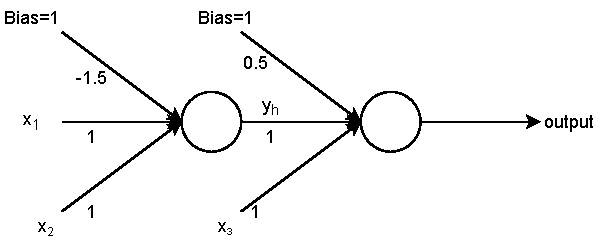
\includegraphics[scale = 0.9]{img/per2.pdf}
								\end{figure}
								con quindi una terza istanza valutata solo nel secondo livello.\\
								La funzione $f$ di attivazione del neurone è definita come quella del
								percettrone, ovvero:
								\[sgn(x)=
									\begin{cases}
										1  & \mbox{se } x\geq 0 \\
										-1 & \mbox{altrimenti}  
									\end{cases}
								\]
								L'esercizio propone di capire la label assegnata a $z_1$ e la label assegnata
								a $z_2$.\\
								Nel dettaglio, per entrambe le istanze, abbiamo $(x_1, x_2, x_3)$, ovvero i
								primi due valori sono (insieme al bias) l'input del primo layer mentre il
								terzo (insieme al bias e al risultato del primo layer) è l'input del secondo
								layer.\\
								Partiamo con $x_1=(0, 2, 2)$.\\
								Si hanno i due layer:
								\begin{enumerate}
									\item nel layer 1 si ha:
									      \[\langle \overline{x},\overline{w}\rangle=
									      	\left(\begin{matrix}
									      	1 & 0 & 2
									      	\end{matrix}\right)
									      	\left(
									      	\begin{matrix}
									      		-1.5 \\
									      		1    \\
									      		1    \\
									      	\end{matrix}
									      	\right)= -1.5+0+2 = 0.5\]
									      	Si ha quindi:
									      	\[\langle \overline{x},\overline{w}\rangle\geq 0\]
									      	e quindi:
									      	\[sgn(\langle \overline{x},\overline{w}\rangle)=sgn(0.5)=1\]
									      	avendo quindi:
									      	\[y_h=1\]
									      	che sarà tra gli input del secondo layer
									      	\item valuto quindi il layer 2:
									      	\[\langle \overline{x},\overline{w}\rangle=
									      		\left(\begin{matrix}
									      		1 & 1 & 2
									      		\end{matrix}\right)
									      		\left(
									      		\begin{matrix}
									      			-0.5 \\
									      			1    \\
									      			1    \\
									      		\end{matrix}
									      		\right)= -0.5+1+2 = 2.5\]
									      		Si ha quindi:
									      		\[\langle \overline{x},\overline{w}\rangle\geq 0\]
									      		e quindi:
									      		\[sgn(\langle \overline{x},\overline{w}\rangle)=sgn(2.5)=1\]
									      		avendo quindi:
									      		\[output=1\]
									      		\end{enumerate}
									      		Possiamo quindi dire che per la prima istanza:
									      		\[f(x_1)=+1\]
									      		Passiamo a $x_2=(1, 0, 0)$.\\
									      		Si hanno i due layer:
									      		\begin{enumerate}
									      			\item nel layer 1 si ha:
									      			      \[\langle \overline{x},\overline{w}\rangle=
									      			      	\left(\begin{matrix}
									      			      	1 & 1 & 0
									      			      	\end{matrix}\right)
									      			      	\left(
									      			      	\begin{matrix}
									      			      		-1.5 \\
									      			      		1    \\
									      			      		1    \\
									      			      	\end{matrix}
									      			      	\right)= -1.5+1+0 = -0.5\]
									      			      	Si ha quindi:
									      			      	\[\langle \overline{x},\overline{w}\rangle< 0\]
									      			      	e quindi:
									      			      	\[sgn(\langle \overline{x},\overline{w}\rangle)=sgn(-0.5)=-1\]
									      			      	avendo quindi:
									      			      	\[y_h=-1\]
									      			      	che sarà tra gli input del secondo layer
									      			      	\item valuto quindi il layer 2:
									      			      	\[\langle \overline{x},\overline{w}\rangle=
									      			      		\left(\begin{matrix}
									      			      		1 & -1 & 0
									      			      		\end{matrix}\right)
									      			      		\left(
									      			      		\begin{matrix}
									      			      			-0.5 \\
									      			      			1    \\
									      			      			1    \\
									      			      		\end{matrix}
									      			      		\right)= -0.5-1+0 = -1.5\]
									      			      		Si ha quindi:
									      			      		\[\langle \overline{x},\overline{w}\rangle < 0\]
									      			      		e quindi:
									      			      		\[sgn(\langle \overline{x},\overline{w}\rangle)=sgn(-1.5)=-1\]
									      			      		avendo quindi:
									      			      		\[output=-1\]
									      			      		\end{enumerate}
									      			      		Possiamo quindi dire che per la prima istanza:
									      			      		\[f(x_2)=-1\]
									      			      		Abbiamo quindi classificato la prima istanza come positiva e la seconda come
									      			      		negativa.
									      			      		\begin{shaded}
									      			      			\textbf{Ripasso di algebra lineare}\\
									      			      			Per praticità ripasseremo i concetti fondamentali facendo riferimento a
									      			      			$\mathbb{R}^2$, formato quindi da elementi, dette coordinate, che sono coppie
									      			      			ordinate $(x_1, x_2)$ (rappresentabili con un punto nel piano o con un segmento
									      			      			orientato con partenza nell'origine e destinazione nelle coordinate del punto
									      			      			nel piano).\\
									      			      			Ricordiamo le operazioni fondamentali, dati $R$ pari a $(x_1, x_2)$ e $Q$ pari
									      			      			a $(x_3, x_4)$ 
									      			      			\begin{itemize}
									      			      				\item addizione: $P+Q=(x_1+x_3, x_2+x_4)$
									      			      				\item prodotto per uno scalare $\lambda\in\mathbb{R}$: $\lambda\cdot
									      			      				      R=(\lambda\cdot x_1,\lambda\cdot x_2)$
									      			      				\item prodotto scalare tra vettori: $\langle P, Q\rangle\equiv P\cdot Q^T =
									      			      				      \sum_{i=1}^n r_i\cdot q_i$ 
									      			      				      (dove $r_i$ e $q_i$ sono rispettivamente gli elementi di $R$ e $Q$
									      			      				      all'indice $i$)
									      			      			\end{itemize}
									      			      			Ricordiamo la \textit{norma} di un vettore $X$:
									      			      			\[\norm{X}=\equiv\sqrt{X\cdot X^T}=\sqrt{\sum_{i=1}^n x_i\cdot
									      			      					x_i}=\sqrt{\langle X, X\rangle}\] 
									      			      				Con $X=0$ indichiamo il \textit{vettore nullo} (che ha anche norma nulla).\\
									      			      				Definiamo il \textit{versore} (\textit{vettore unitario}) come:
									      			      				\[\frac{X}{\norm{X}},\,\,\, X\neq 0\]
									      			      				In $\mathbb{R}^2$ l'angolo $\theta$ sotteso tra due vettori $X$ e $Y$ è:
									      			      				\[\cos\theta=\frac{\langle X, Y\rangle}{\norm{X}\cdot \norm{Y}}\]
									      			      				La proiezione di un vettore $X$ sul vettore $Y$ è:
									      			      				\[X_Y=\norm{X}\cdot \cos\theta\]
									      			      				Si hanno quindi tre casi:
									      			      				\begin{enumerate}
									      			      					\item $\theta < 90 \iff \langle X, Y\rangle >0$
									      			      					\item $\theta > 90 \iff \langle X, Y\rangle <0$
									      			      					\item $\theta = 90 \iff \langle X, Y\rangle =0$
									      			      				\end{enumerate}
									      			      				(quindi disegnando una retta sul piano tutti i punti sopra di essa
									      			      				apparterranno a una certa classe e quelli sotto a un'altra).\\
									      			      				Posso definire una retta $r$ che passa per l'origine in  $\mathbb{R}^2$
									      			      				assegnando un vettore $W=(w_1, w_2)$ ad essa ortogonale, infatti tutti i punti,
									      			      				ovvero vettori, $X=(x_1, x_2)$ sulla retta sono ortogonali a $W$:
									      			      				\[\langle W, X\rangle=w_1\cdot x_1+w_2\cdot x_2=0 \]
									      			      				Quindi la retta (ovvero l'iperpiano) mi separa due semispazi, a seconda che
									      			      				$\langle X, W\rangle$ sia strettamente positivo o strettamente negativo.\\
									      			      				Generalizzando ora a $n$ dimensioni ho che, dato l'iperpiano $h$ (di
									      			      				dimensione $n-1$):
									      			      				\begin{itemize}
									      			      					\item se $h$ passa dall'origine allora si ha l'equazione $\langle X, Y\rangle
									      			      					      =0$
									      			      					\item se non passa per l'origine $\langle X, Y\rangle +b=0$ 
									      			      					          
									      			      				\end{itemize}
									      			      				I vettori in un iperpiano si proiettano tutti nello stesso modo e i punti ad
									      			      				un lato e all'altro dell'iperpiano sono distinti dal fatto che $\langle
									      			      				X, Y\rangle +b$ sia strettamente positiva o strettamente negativa
									      			      				\end{shaded}
									      			      				\end{esercizio}%4

%---------- Support Vector Machines ----- 
\chapter{Support Vector Machines}
\label{Capitolo 5}
Parliamo ora delle \textbf{Support Vector Machines (\textit{SVM})}.\\
Se il percettrone semplice impara solo funzioni di separazione lineari, quello
multistrato anche funzioni di separazione non lineari complesse (ma con
difficoltà di addestramento avendo molti minimi locali e tanti pesi) le SVM
presentano un algoritmo di apprendimento efficiente e imparano funzioni di
separazione non lineari complesse.\\
Viene quindi ripreso comunque il concetto di \textit{separazione lineare} ma con
una scelta efficiente dell'iperpiano, trovando il \textbf{miglior iperpiano
  separatore}, per classificare un insieme di punti linearmente separabili,
trovando un vettore di pesi $W$ per separare bene le istanze. Si usa la
cosiddetto \textbf{teoria statistica dell’apprendimento} che dice che tra tutti
gli iperpiani che possiamo usare per separare due classi si sceglie quello che
sia in grado di etichettare meglio nel futuro. L'intuizione è quella di prendere
un iperpiano ottimo rispetto alla misura della distanza minima che si ha tra gli
esempi, si guardano quindi tutti i punti del training set e cerco di piazzare in
mezzo l'iperpiano, in modo che intorno ad esso ci sii massima ampiezza. Tale
ampiezza è detta margine (volendo che sia massima la distanza minima tra tutti i
punti). SVM usa questa teoria per trovare l'iperpiano ``migliore'' in base a
questi calcoli probabilistici. \\
% magari pic
Non si parla quindi più di neuroni.\\
e riuscissimo a separare i dati con un largo margine
avremmo ragione di credere che il classificatore (ovvero l'iperpiano stesso) sia
``più robusto'' tanto da avere una migliore generalizzazione (assunto che i
punti siano generati da una certa regola).
Quando arriva quindi un nuovo punto, generato con la stessa regola degli altri,
sarà sicuramente classificato correttamente, una volta scelto l'iperpiano.\\
Ci serve quindi la separabilità delle istanze, serve quindi che la funzione
generatrice sia linearmente separabile.
\begin{definizione}[dimensione di Vapnik-Cervonenkis]
  Con la teoria statistica dell'apprendimento si dimostra che più allarghiamo il
  margine meglio l’iperpiano generalizza, raggiungendo la dimensione di
  Vapnik-Cervonenkis (VC).\\
  Prese tutte le funzioni che generano il training set si produce la VC che
  esprime quanto è difficile sbagliare sulle ipotesi future in base alla scelta
  dell'iperpiano.
\end{definizione}
Dobbiamo quindi scrivere un algoritmo per trovare l'iperpiano di separazione di
massimo margine. In input si hanno le istanze etichettate e in output un
vettore che identifica l'iperpiano.\\
Viene usata una notazione matematica che prevede che, preso un insieme di punti
di training:
\[S = \{(x_1, y_1), (x_2, y_2),\ldots, (x_n, y_n)\}\]
a ogni vettore $x_i$ associo la classe di appartenenza $y_i$ (con un etichetta
non booleana):
\[y_i\in\{-1,+1\}\]
Ho i punti linearmente separabili:
\[
  \begin{cases}
    \langle w, x_i\rangle + b >0 &\mbox{se }y_i=+1\\
    \langle w, x_i\rangle + b <0 &\mbox{se }y_i=-1\\
  \end{cases}
\](quindi l'iperpiano separa positivi e negativi)\\
che scritto in un solo vincolo diventa:
\[y_i(\langle w, x_i\rangle + b )>0,\,\,\, i=1,\ldots, n\]
Si ha che $w$ mi dirà quanto è inclinato il piano mentre $b$ è la distanza tra
l'origine e il piano (quindi queste due variabili identificano i vari iperpiani
possibili tra cui cercare il ``migliore'' ovvero quello che separa meglio punti
positivi e negativi).\\
Ci si sposta quindi dalla geometria visualizzabile all'algebra lineare.\\
L'ipotesi quindi tra $w$ e $b$ è una funzione che prende il segno di $<langle
w, x\rangle+b$ per associare l'etichetta:
\[h_{w, b}(x)=sgn(\langle w, x\rangle+b)\]
Date $d_-$ e $d_+$ le distanze tra l’iperpiano separatore e il punto positivo e
negativo più vicino definiamo:
\begin{itemize}
  \item margine funzionale
  \item margine geometrico
\end{itemize}
\begin{definizione}
  Definiamo il \textbf{margine funzionale} di un punto $(x_i, y_i)$ rispetto
  all'iperpiano $(w, b)$ come:
  \[\hat{\gamma}=y_i\cdot(\langle w, x_i\rangle+b)\]
  e quindi il \textbf{margine funzionale} dell'iperpiano rispetto al training
  set $S$ è definito come:
  \[\hat{\rho}=\min_{i=1,\ldots, n}\hat{\gamma_i}\]
\end{definizione}
Si hanno quindi due casistiche:
\begin{enumerate}
  \item se si ha un punto $x_i$ tale che $y_i=+1$, perchè il margine funzionale
  sia grande è necessario che la quantità
  $\langle w, x_i\rangle+b$ abbia un grande valore positivo
  \item se si ha un punto $x_i$ tale che $y_i=-1$, perchè il margine funzionale
  sia grande è necessario che  la quantità
  $\langle w, x_i\rangle+b$ abbia un grande valore negativo
\end{enumerate}
\begin{definizione}
  Se $\hat{\gamma}_i>0,\forall \mbox{classificazione} i$ la classificazione è
  approvata in quanto le classi sono linearmente separabili e l'iperpiano
  $(w, b)$ separa effettivamente le classi
\end{definizione}
Si ha quindi che un ampio margine funzionale fornisce probabilità sulla qualità
della previsione anche se l'uso del solo $\hat{\gamma}$ può essere problematico
in quanto il margine funzionale non è invariante rispetto a un iperpiano
``riscalato''. Analizziamo meglio quest'aspetto.\\
Per come è stato scelto il classificatore $f$ se si scala l'iperpiano:
\[(w, b)\to(c\cdot w, b)\]
si ottengono:
\begin{itemize}
  \item lo stesso iperpiano, ovvero lo stesso luogo di punti
  \item la stessa funzione di decisione, visto che quest'ultima dipende solo dal
  segno di $\langle w, x\rangle+b$, con il segno che può essere invertito se
  $c<0$ 
\end{itemize}
ma dato che il margine funzionale viene moltiplicato per $c$ non possiamo usarlo
come distanza di un punto dall’iperpiano, perché non è invariante rispetto alla
scala.\\
Bisogna ora studiare la distanza $d$ del punto $x$ dall'iperpiano. Si ha quindi:
\[d = \frac{\sum_{i=1}^n w_i\cdot x_i+v}{\norm{w}}=\frac{\langle w,
    x_i\rangle +b}{\norm{w}} \]
Quindi:
\begin{definizione}
  Definiamo il \textbf{margine geometrico} di un punto $(x_i, y_i)$ rispetto
  all'iperpiano $(w, b)$ come:
  \[\gamma_i=\frac{y_i\cdot(\langle w, x_i\rangle+b)}{\norm{w}}\]
  e quindi il \textbf{margine geometrico} dell'iperpiano rispetto al training
  set $S$ è definito come:
  \[\rho=\min_{i=1,\ldots, n}\gamma_i\]
\end{definizione}
\begin{definizione}
  Se $\gamma_i>0,\forall \mbox{classificazione} i$ la classificazione è
  approvata analogamente a quanto detto per il margine funzionale.
\end{definizione}
ato un punto positivo/negativo il margine geometrico rappresenta la sua
distanza geometrica dall'iperpiano. quindi il margine geometrico rende meglio
l'idea della distanza di un punto sa un iperpiano in $\mathbb{R}^n$.\\
Inoltre si ha che \textbf{i margine geometrico è invariante rispetto alla scala
  di $w$} e quindi possiamo ``riscalare'' l'iperpiano senza cambiamenti, non
variando il margine.\\
Dalla formula notiamo che, posto $\norm{w}=1$ si ``riscala'' l'iperpiano $(w, b)$:
\[(w, b)\to\left(\frac{w}{\norm{w}},\frac{b}{\norm{w}}\right)\]
Si considera quindi un iperpiano
$\left(\frac{w}{\norm{w}},\frac{b}{\norm{w}}\right)$ con il vettore di pesi
$\frac{w}{\norm{w}}$ di \textbf{norma unitaria}.
\begin{definizione}
  Definiamo un \textbf{iperpiano canonico} se:
  \[\min_{i=1,\ldots n}|\langle w, x_i\rangle+b|=1\]
  e quindi, per un iperpiano canonico si hanno:
  \begin{itemize}
    \item margine funzionale pari a 1
    \item margine geometrico pari a $\frac{1}{\norm{w}}$
  \end{itemize}
\end{definizione}
Si nota che se $\norm{w}=1$ allora margine funzionale e geometrico coincidono,
infatti si possono mettere in correlazione:
\[\gamma=\frac{\hat{\gamma}}{\norm{w}}\]
Bisogna quindi cercare di estendere il margine, cerchiamo quindi di
massimizzare una certa funzione obiettivo:
\[\max f(x)\]
\[s.t.\,\,\,\,\, g(x)\leq 0\]
\[\qquad h(x)=0\]
Vorremmo assicurarci che tutti i punti (sia quelli positivi sia quelli negativi)
cadano  al di fuori del margine e quindi, dato un certo $\gamma$ vorremmo,
$\forall\, i\in\{1,\ldots, n\}$:
\[\frac{y_i\cdot(\langle w, x_i\rangle+b)}{\norm{w}}\geq \gamma\]
e quindi vogliamo:
\[\max \gamma\]
\[s.t.\qquad y_i\cdot(\langle w, x_i\rangle+b)\leq \gamma\]
\[\norm{w}=1 \]
avendo, con il secondo vincolo,  margine geometrico uguale a quello
funzionale.\\
Riscriviamo quindi:
\[\max \frac{\hat{\gamma}}{\norm{w}}\]
\[s.t.\qquad y_i\cdot(\langle w, x_i\rangle+b)\leq \gamma\]
Non avendo comunque un vincolo convesso.\\
Possiamo però scalare l'iperpiano senza variazioni, grazie all'invarianza. Lo
scalo quindi in modo da avere l'iperpiano canonico, con margine funzionale pari
a 1:
\[\max \frac{1}{\norm{w}}\]
\[s.t.\qquad y_i\cdot(\langle w, x_i\rangle+b)\leq \gamma\]
Si cerca quindi di rendere massimo $\frac{1}{\norm{w}}$ che equivale a rendere
minimo $\frac{1}{2}\norm{w}^2$. Quindi si ottiene che vogliamo minimizzare
$\frac{1}{2}\norm{w}^2$, che per comodità chiamiamo $\tau(w)$:
\[\min \tau(w)=\frac{1}{2}\norm{w}^2\]
\[s.t.\quad y_i\cdot(\langle w, x_i\rangle+b)\leq \gamma\]
\begin{definizione}
  Si dimostra che esiste una sola soluzione al problema, ovvero esiste un unico
  iperpiano di massimo margine.
\end{definizione}
Ricapitolando si hanno due ragioni a supporto delle SVM:
\begin{enumerate}
  \item la \textbf{generalizzazione}, ovvero la capacità dell'iperpiano di
  separazione di massimo margine
  \item esiste un’unica soluzione del problema di ottimizzazione appena
  descritto 
\end{enumerate}


Si sta cercando:
\[\min \tau(w)=\frac{1}{2}\norm{w}^2\]
\[s.t.\quad y_i\cdot(\langle w, x_i\rangle+b)\leq \gamma\]
e si ha che:
\[w=\sum_{i\in Q}\alpha_i\cdot x_i\]
Ovvero scritta in termini di un sottoinsieme di esempi del training set (noto
come vettori di supporto) che giacciono sul margine dell’iperpiano, prendendo
una somma pesata dei contenuti dei vettori.\\
% pic pagina 36
Il passaggio finale è che se ho $\langle w, x\rangle+b$ che indicano cosa ho
appreso, se ricevo un vettore $x$ da classificare posso determinare l'etichetta:
\[sgn(\langle w, x\rangle+b)=sgn\left(\Big\langle\sum_{i\in Q}\alpha_i\cdot
    x_i, x\Big\rangle +b\right)=sgn\left(\sum_{i\in Q}\alpha_i\langle x_i, x\rangle
    +b\right)\]
Quindi la funzione di decisione associata alla soluzione può essere scritta in
termini del prodotto interno tra i vettori di supporto (\textit{support vector})
$x_i$ e il vettore da classificare $x$.\\
$\alpha$ viene elaborato dai vettori di supporto ma non verrà ora trattato.\\
Passiamo quindi oltre alla sola separabilità lineare.\\
Si usa lo stesso approccio rivedendo la formulazione tramite i \textbf{metodi
  kernel}. Si cerca di mappare lo spazio d'input in un nuovo spazio, (in
generale di dimensione maggiore), in cui i punti siano linearmente separabili,
per classificare mediante superfici non lineari.\\
% immagine pagina 39
Dobbiamo trovare una funzione:
\[\Phi:\mathbb{R}^n\to \mathbb{R}^m,\mbox{con }m>n\]
chemappi i dati iniziali non linearmente separabili in uno spazio di dimensione
superiore in cui siano linearmente separabili.\\
In questo nuovo spazio la funzione di decisione che classifica l'input $x$ è:
\[sgn\left(\sum_{i\in Q}\alpha_i\langle \Phi(x_i),\Phi(x)\rangle+b\right)\]
Il calcolo delle funzioni $\Phi$ è generalmente computazionalmente pesante ma è
semplificato nel caso di \textbf{funzioni kernel}.
\begin{definizione}
  Definiamo una \textbf{funzione kernel}. Data una trasformazione
  $\Phi:\mathbb{R}^n\to \mathbb{R}^m$ una \textbf{funzione kernel} è una mappa:
  \[K:\mathbb{R}^n\times \mathbb{R}^n\to \mathbb{R}\mbox{
      t.c. }K(x, y)=\Phi(x)\cdot \Phi(y)\]
\end{definizione}
\begin{definizione}
  Si definisce quindi il \textbf{kernel trick} che consiste nel computare il
  prodotto interno delle trasformare di due vettori $x$ e $y$, tramite $\Phi$,
  senza computare le trasformate, semplificando il calcolo di:
  \[sgn\left(\sum_{i\in Q}\alpha_i\langle \Phi(x_i),\Phi(x)\rangle+b\right)\]
  sostituendo $\Phi(x_i)\cdot\Phi(x)$ con $K(x_i, x)$, ottenendo:
  \[sgn\left(\sum_{i\in Q}\alpha_i\cdot K(x_i, x)+b\right)\]
  con:
  \[K(x, y)=\langle \Phi(x),\Phi(y)\rangle\]
  Non si cercano tutte le possibili trasformazioni ma solo alcune.
\end{definizione}
\begin{esempio}
  Sia:
  \[\Phi:\mathbb{R}^2\to \mathbb{R}^3\]
  con rispettivamente $(x, y)$ e $(r, s, t)$\\
  tale che;
  \[r=x^2,\,\, s=y^2,\,\, t=\sqrt{2xy}\]
  presi $p_1=(x_1, y_1), p_2=(x_2, y_2\in\mathbb{R}^2$ ho il loro prodotto interno
  delle loro immagini in $\mathbb{R}^3$:
  \[(x_1^2, y_1^2,\sqrt{2x_1y_1})\cdot
    [(x_2^2, y_2^2,\sqrt{2x_2y_2})=(x_1x_2)^2+(y_1y_2)^2+2x_1x_2x_2y_2\]
  ma questo è il quadrato del prodotto interno tra $p_1$ e $p_2$:
  \[[(x_1, y_1)+(x_2, y_2)]^2=(x_1x_2+y_1y_2)^2\]
  non dovendo quindi calcolare immagini in $\mathbb{R}^3$
\end{esempio}
% immagine pagina 26
Si hanno alcune proprietà:
\begin{itemize}
  \item se i dati sono mappati in uno spazio di dimensioni sufficientemente
  elevate, saranno quasi sempre linearmente separabili
  \item quattro dimensioni sono sufficienti per separare linearmente un cerchio
  in qualsiasi punto del piano
  \item cinque dimensioni sono sufficienti per separare linearmente qualsiasi
  ellisse
  \item se abbiamo $N$ esempi sono sempre separabili in spazi di dimensioni
  $N-1$ o più
  \item calcolare $K(x, y)$ può essere molto economico anche se $\Phi(x)$ è molto
  costoso, ad esempio con vettori di dimensione elevata e, in tali casi (che
  vanno dimostrati), si
  addestrano le SVM nello spazio di dimensionalità maggiore senza mai dover
  trovare o rappresentare esplicitamente i vettori $\Phi(x)$
\end{itemize}
\begin{esempio}
  Si data la trasformazione:
  \[\Phi:\mathbb{R}^3\to \mathbb{R}^{10}\]
  tale che:
  \[\Phi(x)=(1,
    \sqrt{2x_1},\sqrt{2x_2},\sqrt{2_3},\sqrt{2x_1x_2},\sqrt{2x_1x_3},
    \sqrt{2_1x_3}, x_1^2, x_2^2, x_3^2)\]
  ovvero i 10 possibili monomi fino al grado due ottenuti da tre variabili. Si
  ha che:
  \[\Phi(x)\cdot\Phi(y)=1+2\cdot\sum_1^dx_iy_i+2\cdot\sum_1^dx_i^2y_i^2+2\cdot\sum_{i, j}
    x_ix_jy_iy_j=(1+xy)^2\]
  
\end{esempio}
Vediamo una lista di kernel standard:
\begin{itemize}
  \item \textbf{lineare}:
  \[K(x, y)=x\cdot y\]
  \item \textbf{polinomiale}:
  \[K(x, y)=(1+x\cdot y)^d\]
  \item \textbf{radial basis function}:
  \[K(x, y)=e^{-y\norm{x-y}^2}\]
  \item \textbf{gaussian radial basis function}:
  \[K(x, y)=e^{-\frac{(x-y)^2}{2\sigma^2}}\]
  \item \textbf{percettrone multistrato}:
  \[K(x, y)=\tanh (b(x\cdot y) -c)\]
\end{itemize}
\begin{definizione}
  Un kernel definisce una matrice $K_{ij}$ che è simmetrica e definita positiva
\end{definizione}
\begin{definizione}[definizione di Mercer]
  Ogni matrice simmetrica e definita positiva è un kernel
\end{definizione}
SVM può essere applicato a problemi non binari tramite il \textbf{one vs rest},
avendo separazioni a più classi. Spesso posso ridurmi comunque a sottoproblemi
binari, avendo più gruppi di punti linearmente separabili. SVM trova quindi
tutte le possibili separazioni lineari. Combinando quindi i risultati ottenuti
sui sottoproblemi binari derivati, risultati ottenuti con SVM, e definendo una
logica di classificazione per il problema originale posso fare un'analisi
multiclasse.\\
Si ha quindi l'addestramento di un singolo classificatore per classe, con i
campioni di quella classe come campioni positivi e tutti gli altri campioni come
negativi.\\
Questa strategia richiede che i classificatori di base producano un punteggio di
confidenza a valore reale per la sua decisione, piuttosto che solo un'etichetta
di classe, infatti le sole etichette di classi discrete possono portare a
ambiguità.
\newpage
Abbiamo quindi:
\begin{itemize}
  \item come input:
  \begin{itemize}
    \item un learner $L$
    \item un set di esempi $X$
    \item delle label $y_i$ associate ad ogni $x_i\in X$ con $i=1,\ldots K$
  \end{itemize}
  \item come output una lista di classificatori $f_k$ con $l=1,\ldots K$
\end{itemize}
La procedura è quindi, $\forall k\in \{1\ldots K\}$ costruisco un nuovo vettore
di label $z$ tale che:
\[
  \begin{cases}
    z_i=y_i&\mbox{se } y_i=k\\
    z_i=0&\mbox{altrimenti}
  \end{cases}
\]
applicando poi $L$ a $(X, z)$ per ottenere $f_k$.\\
Quindi prendere decisioni significa applicare tutti i classificatori a un nuovo
sample e prevedere l'etichetta $k$ er la quale il classificatore corrispondente
riporta il punteggio di confidenza più alto:
\[\hat{y}=argmax\,\, f_k(x),\,\,\, k\in\{1,\ldots K\}\]
Questa euristica soffre di diversi problemi:
\begin{itemize}
  \item la scala dei valori di confidenza può differire tra vari classificatori
  binari 
  \item anche se la distribuzione in classe è bilanciata nel training set, i
  learner per la classificazione binaria vedono distribuzioni sbilanciate
  perché tipicamente l'insieme di negativi che vedono è molto più grande
  dell'insieme di positivi
\end{itemize}
Un'alternativa è il \textbf{one vs one} prendendo le varie classi e produrre
sistemi di SVM tra coppe di classe. La quantità di problemi derivati esplode in
modo quadratico. Alla fine si attribuisce maggior probabilità a una singola
classe.\\
Si ha il train di:
\[\frac{K\cdot (K-1)}{2}\]
classificatori binari per un problema a $K$ classi e ognuno riceve i campioni di
un paio di classi dal training set originale e deve imparare a
distinguere queste due classi.\\
In fase di predizione tutti i $\frac{K\cdot (K-1)}{2}$ classificatori sono
applicati al nuovo sample e la classe che con il più alto numero di predizioni
positive viene usata come previsione per il classificatore combinato. Anche
questa tecnica soffre di ambiguità in quanto alcune regioni del suo spazio di
input possono ricevere lo stesso numero di voti.
\subsubsection{Esercitazione su SVM e metodi kernel}
\textbf{Nell'esercitazione ogni $\vec{w}\cdot\vec{x}$ è da caloclarsi come
  $\vec{w}^T\cdot\vec{x}$.} 
\begin{definizione}
  Definiamo \textbf{iperpiano} su uno spazio euclideo a $n$ dimensioni come un
  sottoinsieme piatto di $n-1$ dimensioni che divide lo spazio in due parti non
  connesse. \\
  È quindi un luogo di punti che soddisfa:
  \[\vec{w}\cdot\vec{x}+b=0\]
  Ovviamente:
  \begin{itemize}
    \item in una dimensione è un punto
    \item in due dimensioni una retta
    \item in tre dimensioni un piano
    \item in più di tre dimensioni si usa direttamente il termine iperpiano
  \end{itemize}
  Nel caso a due dimensioni, per esempio, si ha che:
  \[\vec{w}\cdot\vec{x}+b=0\]
  (che in due dimensioni è la forma implicita di una retta) corrisponde a:
  \[w_0x+w_1y+b=0\]
  ovvero:
  \[w_1y=-w_0x-b\]
  Isolo quindi $y$:
  \[y=-\frac{w_0}{w_1}x-\frac{b}{w_1}\]
  e avendo:
  \begin{itemize}
    \item $m=-\frac{w_0}{w_1}$ come coefficiente angolare
    \item $q=-\frac{b}{w_1}$ come ordinata origine della retta, il punto di
    intercetta 
  \end{itemize}
  ottengo la classica equazione della retta, in forma esplicita:
  \[y=mx+q\]
  Quindi $\vec{w}\cdot\vec{x}+b$ assegna una sorta di ``punteggio''.

\end{definizione}
\begin{esempio}
  Preso $\vec{w}=(-0.4,-1)$ e $b=9$ si studino i punti $A(1, 3)$, $B(3, 5)$ e
  $C(5, 7)$.\\
  Si ottiene:
  \begin{itemize}
    \item per $A$, con $\vec{x}=(1, 3)$, si ha $\vec{w}\cdot\vec{x}+b=5.6$
    \item per $B$, con $\vec{x}=(3, 5)$, si ha $\vec{w}\cdot\vec{x}+b=2.8$
    \item per $C$, con $\vec{x}=(5, 7)$, si ha $\vec{w}\cdot\vec{x}+b=0$
  \end{itemize}
  Avendo che $C$ giace sull'iperpiano (l'equazione è nulla) e gli altri punti,
  essendo in due dimensioni e quindi avendo a che fare con una retta, sono sotto
  la retta ($A$ più lontano di $B$ avendo ``punteggio'' maggiore).
\end{esempio}
Con il percettrone si vedeva se i punti erano linearmente separabili (trovando
un iperpiano che separava) con SVM si cerca l'iperpiano ottimo per separare i
punti.
\begin{esempio}
  Sia data una funzione d'ipotesi (che definisce un'ipotesi in $H$) tale che:
  \[h(\vec{x}_i=
    \begin{cases}
      +1&\mbox{se }\vec{w}\cdot\vec{x}_i+b\geq 0\\
      -1&\mbox{se }\vec{w}\cdot\vec{x}_i+b< 0
    \end{cases}
  \]
  ovvero:
  \[h(\vec{x_i}=sign(\vec{w}\cdot\vec{x}_i+b)\]
  quindi i valori positivi sono sopra etichettati come positivi e i negativi
  come  negativi.\\
  Siano dati:
  \begin{itemize}
    \item $\vec{w}=(0.4, 1)$
    \item $b=-9$
    \item $A(8, 7)$ e $B(1, 3)$
  \end{itemize}
  Si ha:
  \begin{itemize}
    \item per $A$, che è sopra l'iperpiano:
    \[\vec{w}\cdot\vec{x}_i+b=0.4\cdot 8+1\cdot 7-9=1.2\]
    quindi è etichettato come positivo
    \item per $B$, che è sotto l'iperpiano:
    \[\vec{w}\cdot\vec{x}_i+b=0.4\cdot 1+1\cdot 3-9=-5.6\]
    quindi è etichettato come negativo
  \end{itemize}
  Ma non si è detto nulla sulla scelta dell'iperpiano, ne in termini di calcolo
  ne in termini studio della sua qualità.
\end{esempio}
Ci serve quindi una misura di confidenza per la classificazione usando i
\textbf{margini}. \\
Abbiamo quindi il punteggio $\beta$ dato da:
\[\beta=\vec{w}\cdot\vec{x}+b\]
e perché tale punteggio sia utile ci serve anche la classe di appartenenza
$y$. Si ha quindi:
\[f=y\cdot\beta\implies f=y\cdot(\vec{w}\cdot\vec{x}+b)\]
avendo ottenendo il \textbf{margine funzionale} $f$ tale che:
\begin{itemize}
  \item $f$ è positivo se la classificazione è corretta
  \item $f$ è negativo se la classificazione non è corretta
\end{itemize}
Inoltre:
\begin{itemize}
  \item se si ha $y=1$ allora affinché il margine funzionale sia ampio (cioè,
  affinché la nostra previsione sia sicura e corretta), allora abbiamo bisogno
  che $\vec{w}\cdot\vec{x}+b$ sia un numero positivo grande 
  \item se si ha $y=-1$ allora affinché il margine funzionale sia grande, allora
  abbiamo bisogno che $\vec{w}\cdot\vec{x}+b$ sia un grande numero negativo 
\end{itemize}

Per una certa osservazione $i$ si ha quindi (usiamo la dicitura $\hat{gamma}$ al
posto di $f$ per il margine funzionale):
\[\hat{\gamma}^{(i)}=y^{(i)}(\vec{w}\cdot\vec{x}+b)\]
e quindi per tutti i dati si cerca:
\[\hat{\gamma}=\min \hat{\gamma}^{(i)}\]
Ma si ha ancora un problema: dipende dalla scala. Se a $\vec{w}$ sostituiamo,
ad esempio, $2\vec{w}$ e a $b$ sostituiamo $2b$ si ha che la classificazione
fatta con $sign(\vec{w}\cdot\vec{x}_i+b)$ resta la medesima (anche perché
l'iperpiano resta lo stesso, avendo dipendenza lineare). D'altro canto il
margine funzionale aumenta all'aumentare dei due valori (aumentando lo score) e
quindi si ha una ``falsa'' confidenza (sembrando due volte più confidente quando
è tutto uguale in realtà, dall'iperpiano alla classificazione).\\
Si introduce quindi il \textbf{margine geometrico}, dividendo il margine
funzionale per la norma di $\vec{w}$:
\[\hat{\gamma}^{(i)}=y^{(i)}\left(\frac{\vec{w}}{\norm{\vec{w}}}
    \cdot\vec{x}^{(i)}+\frac{b}{\norm{\vec{w}}}\right)\]
si ha quindi un invaiante rispetto al fattore di scala, a differenza del margine
funzionale (con la divisione per la norma semplifico eventuali fattori
moltiplicativi costanti).\\
Anche in questo caso cerco il minimo:
\[\hat{\gamma}=\min \hat{\gamma}^{(i)}\]
Con SVM si cerca l'iperpiano ottimo ovvero che massimizza il margine per
entrambe le classi considerate nel training set, rendendo massima la distanza
tra i punti più vicini di ogni classe, minimizzando il margine geometrico di
ogni esempio. Si trovano i support vector dove giacciono i più vicini punti
all'iperpiano per le due classi. Il risultato dell'ottimizzazione per SVM è
trovare il gap maggiore che ci separa da tutte le classi contemporaneamente
\begin{figure}[H]
  \centering
  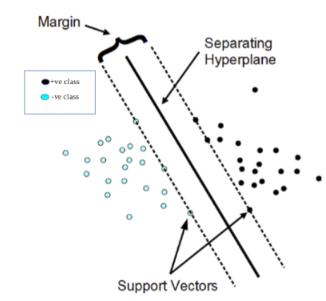
\includegraphics[scale = 0.7]{img/svm.jpg}
  \caption{Visualizzazione di SVM}
  \label{fig:svm}
\end{figure}
Se non si può separare positivi dai negativi (o un training set non linearmente
separabile) in uno spazio di bassa dimensione
utilizzando un iperpiano, bisogna mappare tutto in uno spazio dimensionale
superiore dove è possibile separarli, tramite i \textbf{metodi kernel}. Tramite
una funzione $\phi$ si passa lo spazio d'input in uno nuovo, detto
\textbf{feature space}, a dimensione maggiore, dove i punti sono linearmente
separabili.  
\begin{esempio}
  Dato $[x^{(1)}, x^{(2)}]$ si ha:
  \[\phi([x^{(1)}, x^{(2)}])=[x^{(1)2}, x^{(2)2}, x^{(1)}x^{(2)}]\]
  facendo, in questo esempio, il quadrato delle due componenti e il loro
  prodotto, da due dimensioni passo a 3.
\end{esempio}
\begin{definizione}
  Dato uno spazio delle istanze $X$ e un feature space $F$ si ha che una
  funzione $k$:
  \[k_X\to X\times X\to\mathbb{R}\]
  è detta kernel valido sse esiste una \textit{feature map} $\phi$:
  \[\phi:X\to F\]
  tale che:
  \[k(x, z)=\langle\phi(x),\phi(z)\rangle,\,\,\,\forall\, x, z\in X\]
  avendo quindi che posso rappresentare $k$ tramite un prodotto interno di
  feature risultate dal mapping definito da $\phi$.\\
  La funzione $k$ ha quindi come argomenti due vettori senza restrizioni,
  potendo mappare un ampio spettro di entità (documenti, proteine etc$\ldots$),
  può quindi essere penata come una \textbf{funzione si similarità} (pensata
  come prodotto euclideo), dicendo
  quanto sono simili gli oggetti della funzione kernel.\\
  Avendo il prodotto interno scalare si ha anche la norma, dando prova della
  lunghezza del vettore, e avendo anche la \textbf{distanza} tra due vettori
  nello spazio, che all'inverso è una misura di similarità.
\end{definizione}
\begin{definizione}
  Definiamo \textbf{kernel matrix}, detta anche \textbf{gram matrix}, dato un
  kernel $k$ e un insieme 
  $S=x_1, x_2,\ldots x_n$, come una matrice dove ogni componente è:
  \[G_{i, j}=\langle\phi(x_i),\phi(x_j)\rangle_{\mathcal{H}}=k(x_i, x_j)\]
\end{definizione}
Molti algoritmi interagiscono coi dati tramite prodotti scalari per questo sono
importanti le funzioni kernel. Per definizione di kernel posso quindi sostituire
un prodotto interno tra due vettori con la funzione kernel definita sui quei due
vettori, spostandomi in una dimensione maggiore per il feature space e ottenendo
un valore di similarità tra i due oggetti. 
\begin{esempio}
  Vediamo un esempio di funzione kernel. \\
  Siano dati:
  \begin{itemize}
    \item $\vec{x}=(x_1, x_2)$
    \item $\vec{z}=(z_1, z_2)$
    \item $dim=2$
  \end{itemize}
  Si ha quindi:
  \[(\vec{x}\cdot\vec{z})^2=(x_1z_1+x_2z_2)^2
    =(x_1^2x_2^2+x_2^2z_2^2+2x_1z_1x_2z_2)\]
  \[=\langle\left(x_{1}^{2}, x_{2}^{2}, \sqrt{2} x_{1}
      x_{2}\right),\left(z_{1}^{2}, z_{2}^{2}, \sqrt{2} z_{1}
      z_{2}\right)\rangle=\langle\phi(\vec{x}),\phi(\vec{z})\rangle\]
  Avendo ottenuto le feature. Quindi la funzione iniziale è rappresentabile come
  il prodotto interno tra le due feature, in modo implicito.\\
  Avendo quindi:
  \[\phi(x_1, x_2)=(x_1^2, x_2^2,\sqrt{2}x_1x_2\]
  \[\phi(xz_1, z_2)=(z_1^2, z_2^2,\sqrt{2}z_1z_2\]
  passando a $dim=3$.
\end{esempio}
Tra i tipo di kernel si segnala quello gaussiano:
\[ k(\mathbf{x}, \mathbf{z}) =\exp \left(-\frac{\|\mathbf{x}-
      \mathbf{z}\|^{2}}{2 \sigma^{2}}\right) 
  =\exp \left(-\frac{\mathbf{x}^{\mathbf{T}} \mathbf{x}-\
      mathbf{2} \mathbf{x}^{\mathbf{T}} \mathbf{z}+
      \mathbf{z}^{\mathbf{T}} \mathbf{z}}{2 \sigma^{2}}\right)\]
La strategia di kernel di un algoritmo è che ogni volta che si trova un prodotto
interno di feature si ha che questo è uguale al kernel nello spazio
originale. Non serve conoscere il mapping se il kernel è valido e posso quindi
procedere direttamente con la sostituzione.
\begin{definizione}
  Un metodo è detto \textbf{kernelizzato} se il prodotto interno delle sue
  feature può essere valutato da una qualunque funzione kernel nello spazio di
  rappresentazione originale.
\end{definizione}
Le distanze e le differenze sono state questioni importanti nel machine
learning e nel riconoscimento di modelli per molti anni, portando a molti
algoritmi noti diversi e domande importanti.\\
La distanza tra oggetti nello spazio delle feature è definita da:
\[d(x, x_2)=\norm{\phi(x)-\phi(x_2)}^2_{\mathcal{H}}\]
denotando con $\mathcal{H}$ lo spazio del prodotto interno dove le feature sono
rappresentate dal mapping:
\[\phi:X\to \mathcal{H}\]
Si ha quindi per la distanza, estendendo la norma:
\[
  \left\|\Phi\left(x_{1}\right)-\Phi\left(x_{2}\right)\right\|_{\mathcal{H}}^{2}
  =<\Phi\left(x_{1}\right)-\Phi\left(x_{2}\right),
    \Phi\left(x_{1}\right)-\Phi\left(x_{2}\right)>\]
    \[
  =<\Phi\left(x_{1}\right), \Phi\left(x_{1}\right)>-2<\Phi
  \left(x_{1}\right), \Phi\left(x_{2}\right)>+<\Phi\left(x_{2}\right),
  \Phi\left(x_{2}\right)>
\]
e con la notazione kernel, avendo sostituito con un kernel valido $k$, ottenendo
una riscrittura della distanza tra due feature, kernelizzando la distanza tra
due input:
\[\left\|\Phi\left(x_{1}\right)-\Phi\left(x_{2}\right)\right\|_{\mathcal{H}}^{2}
  =k(x_1, x_1)-2k(x_1, x_2)+k(x_2, x_2)\]
\textbf{Si hanno liste di funzioni kernel verificate.} %5

%---------- Apprendimento Bayesano ----- 
\chapter{Apprendimento Bayesiano}
In questo capitolo considereremo l'apprendimento come una forma di ragionamento incerto sulle osservazioni. Sappiamo che l'incertezza è prevalente negli ambienti reali e gli agenti possono gestirla mediante metodi probabilistici. Per far ciò però essi devono apprendere una loro teoria probabilistica del mondo circostante. Il punto di vista Bayesiano sull'apprendimento è estremamente potente ed offre soluzioni generali ai problemi del rumore, del sovradattamento e della predizione ottima. Viene anche considerato il fatto che un agente non onnisciente non potrà mai essere certo della correttezza di una teoria sul mondo ma deve comunque utilizzarne una per prendere delle decisioni, per cui viene sfruttata \textbf{solitamente} l'ipotesi più probabile. Nell'ambito Bayesiano si cambia l'approccio avendo la valutazione d'ipotesi in base alla loro probabilità. Si studia la probabilità rispetto ai dati e rispetto alle conoscenze pregresse. Non troviamo quindi un'ipotesi perfettamente compatibile ma una che è più probabile rispetto ad altre. Bisogna dunque studiare come scegliere le ipotesi, usando risultati noti del calcolo
probabilistico. Useremo le nozioni di probabilità e probabilità condizionata, oltre ovviamente alla \textbf{regola di Bayes}.
Si assume quindi che le quantità d'interesse siano ``governate'' da
distribuzioni di probabilità e che la decisione migliore può essere presa ragionando su tali distribuzioni e sull'insieme di dati di
training. L'apprendimento Bayesiano è importante per due ragioni principali:
\begin{enumerate}
  \item si ha una manipolazione esplicita delle probabilità rispetto ad altri approcci pratici di alcuni tipi di problemi di apprendimento (infatti si hanno
  spesso paragoni con gli alberi decisionali e con le reti neurali)
  \item fornisce una prospettiva utile per comprendere metodi di apprendimento
  che non manipolano effettivamente le probabilità
\end{enumerate}
\section{Apprendimento Statistico}
I concetti chiave sono i \textbf{dati} e le \textbf{ipotesi}. I dati rappresentano \textbf{prove}, ovvero istanziazioni di alcune o tutte le \textbf{\href{https://it.wikipedia.org/wiki/Variabile_casuale}{Variabili Casuali}} che descrivono il dominio. Le ipotesi invece esprimono  teorie probabilistiche sul funzionamento del dominio.
Dal punto di vista delle funzionalità si ha che ogni esempio di training osservato può aumentare o diminuire, in modo incrementale, la stima di probabilità relativa alla correttezza di un'ipotesi. Inoltre, come già anticipato, la conoscenza pregressa può essere combinata con i dati osservati per determinare la probabilità finale delle varie ipotesi. In particolare si afferma inoltre che le
varie ipotesi possono effettuare predizioni probabilistiche e le istanze possono essere quindi classificate combinando le predizioni delle varie ipotesi, che sono pesate tramite il peso delle loro probabilità. Con il metodo Bayesiano si ottiene quindi uno ``standard'' per prendere decisioni ottimali rispetto al quale è possibile misurare ulteriori misure pratiche.\\
Si hanno però alcune difficoltà legate all'apprendimento Bayesiano:
\begin{itemize}
  \item si necessita avere la conoscenza di varie probabilità
  \item si hanno costi computazionali non indifferenti
\end{itemize}
\subsection{Probabilità a priori delle ipotesi e Verosimiglianza}
\begin{definizione}[Apprendimento Bayesiano]
L'apprendimento Bayesiano calcola semplicemente la probabilità di ogni ipotesi condizionandola ai dati osservati,  e su tale base formula predizioni. Le predizioni possono essere quindi basate su tutte le ipotesi, pesate secondo la rispettiva probabilità, e non solo su quella migliore.
\end{definizione}
% Inquadrando nuovamente il fulcro del machine learning ricordiamo che si sta
% cercando la ``miglior'' ipotesi $h$, contenuta dello spazio delle ipotesi $H$, a
% partire dai dati contenuti in un training set $D$. Nell'apprendimento Bayesiano
% si ha che la ``miglior'' ipotesi altro non è che la più probabile. Ovviamente
% potrebbero esistere più ipotesi. 
La \textbf{formula di Bayes} fornisce un metodo diretto per calcolare la probabilità di tale ipotesi in base:
\begin{itemize}
  \item alla sua probabilità conosciuta a priori
  \item alle probabilità di osservare vari dati data l'ipotesi
  \item ai dati stessi
\end{itemize}
\begin{definizione}[Definizione di Bayes]
  Preso il DataSet \textbf{d}, allora definiamo la distribuzione di probabilità a \textbf{posteriori}:
  \[P(h_i|d)=\frac{P(d|h_i)P(h_i)}{P(d)}\]
  Dove:
  \begin{itemize}
        \item $P(h_i)$ viene chiamata \textbf{probabilità a priori delle ipotesi}
        \item $P(d|h_i)$ è la \textbf{verosimiglianza} dei dati sotto ogni ipotesi.
        \item $P(d)$ che è la probabilità conosciuta a priori di del dataset, ovvero la
     probabilità che esso sia osservato.\\ Si calcola come: $P(d)=\sum_i(d, h_i)=\sum_i P(d|h_i)P(h_i)$
    \end{itemize}
%   \begin{itemize}
%     \item $P(h)$ che è la probabilità conosciuta a priori di $h$. Tale
%     probabilità riflette qualsiasi conoscenza di base sulla possibilità
%     che $h$ sia corretta  
%     \item $P(d)$ che è la probabilità conosciuta a priori di $D$, ovvero la
%     probabilità che $D$ sia osservato
%     \item $P(d|h)$ che è la probabilità di osservare $D$ in presenza
%     dell'ipotesi $h$
%     \item $P(h|d)$ che è la probabilità a posteriori di $h$. Tale probabilità
%     riflette la ``confidenza'' di avere $h$  dopo che $D$ è stato osservato
%   \end{itemize}
\end{definizione}
\begin{definizione}
Sia \textbf{D} il DataSet dove i valori osservati vengono indicati con \textbf{d}. Supponiamo di voler predire una predizione $"X"$:
\begin{equation}
    P(X|d)=\sum_{i}P(X|d, h_i)P(h_i|d) = \sum_{i}P(X|h_i)P(h_i|d) 
    \label{Bayes}
\end{equation}
\begin{nota}
    Abbiamo presunto che ogni ipotesi determini una distribuzione di probabilità $X$. Quest'equazione mostra che le predizioni sono medie pesate delle predizioni delle singole ipotesi. Le ipotesi stesse fungono essenzialmente da \textit{intermediari} tra i dati nudi e le predizioni.
\end{nota}
\end{definizione}
La figura \ref{fig:Prob2} mostra la predizione della probabilità che l'osservazione successiva abbia una data classificazione, seguendo la \ref{Bayes}. 
\begin{figure}[H]
    \centering
    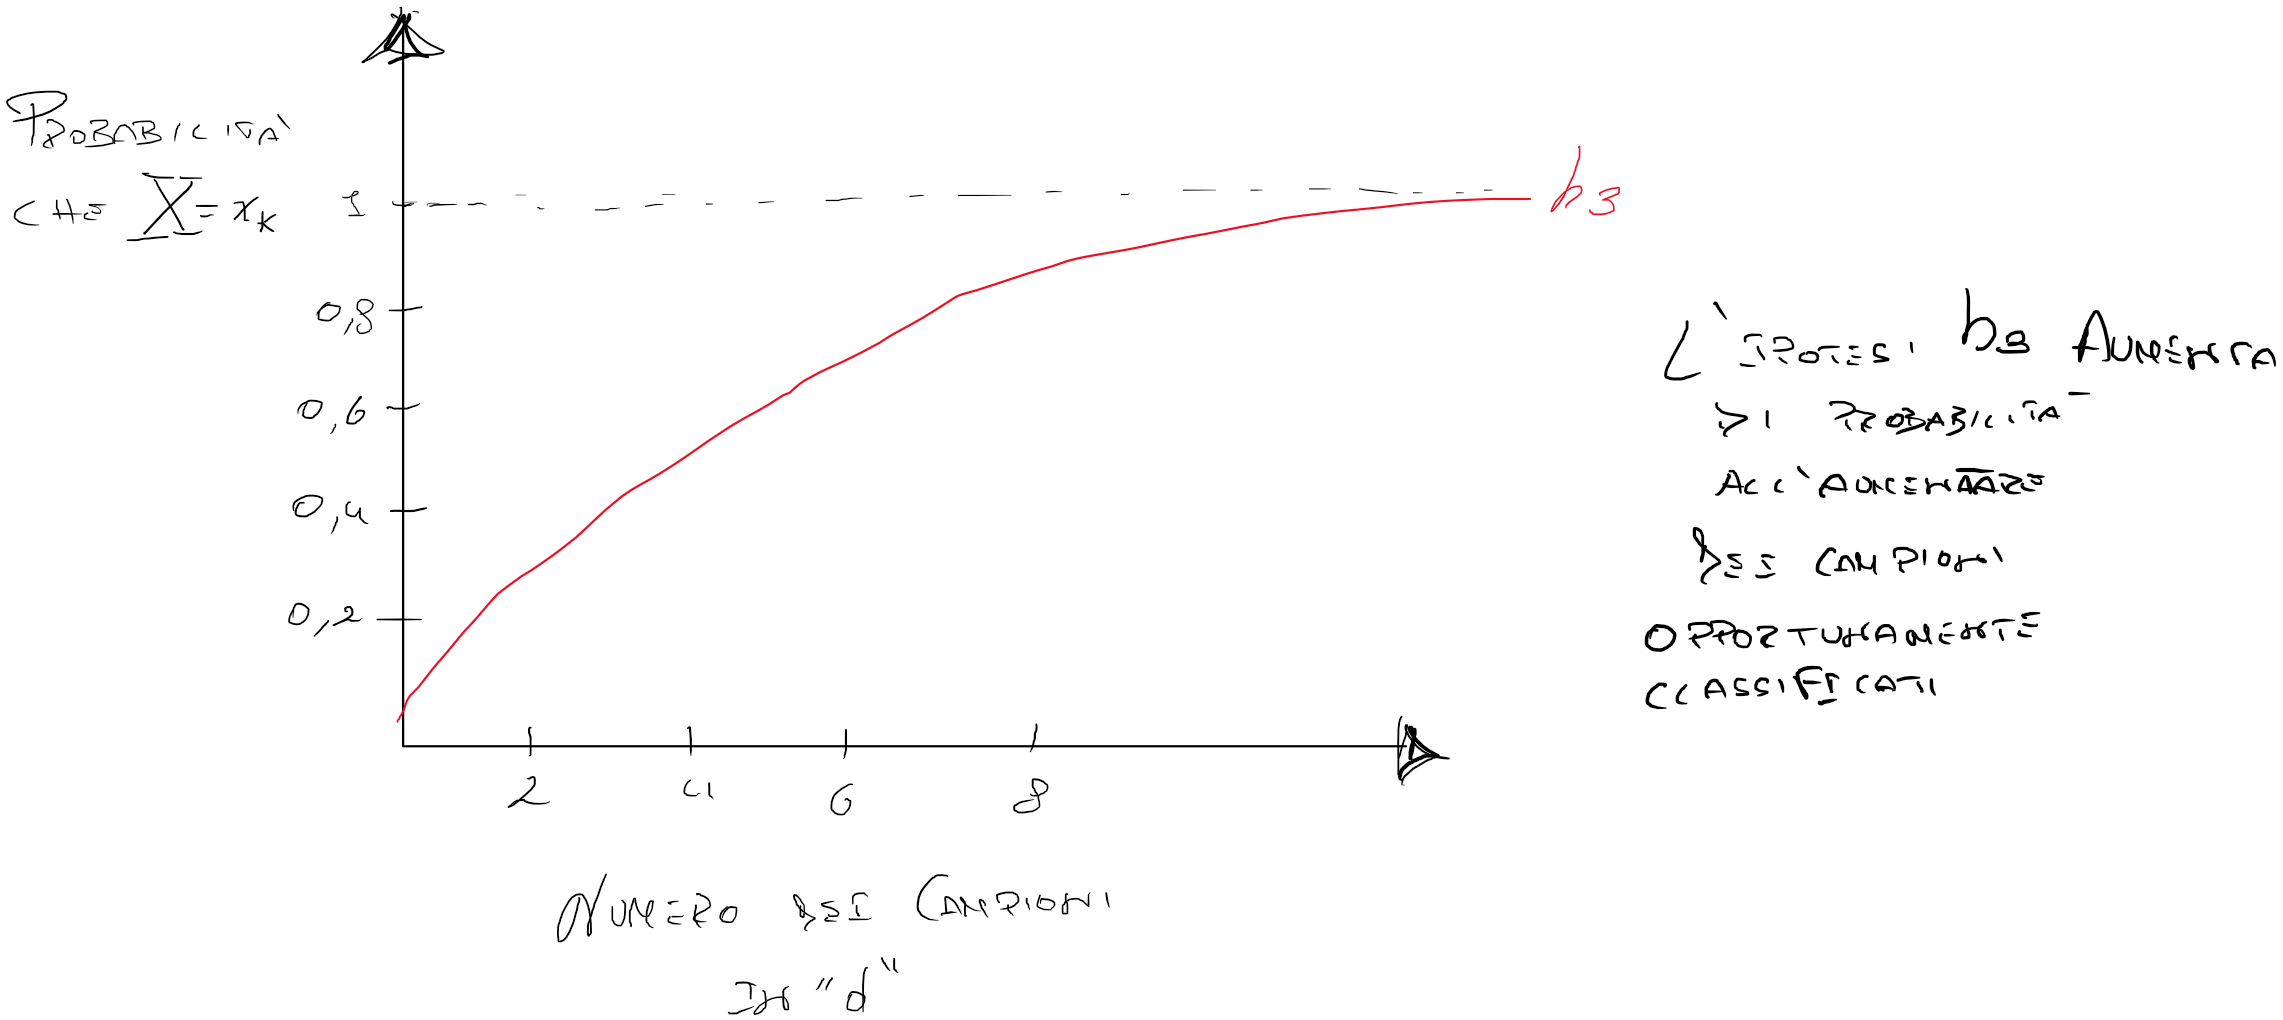
\includegraphics[width=1\textwidth]{img/prob2.png}
    \caption{Predizione bayesiana $P(d_{n+1} = x_k | d1 \dots d_n)$}
    \label{fig:Prob2}
\end{figure}
\begin{definizione}[Verosimiglianza]
  La verosimiglianza dei dati è calcolata partendo dal presupposto che le osservazioni $d_j$ in un dataset \textbf{d}, siano indipendentemente e identicamente distribuite (\textbf{i.i.d}), così che:
  \[P(d|h_i)=\prod_{j}P(d_j|h_i)\]
\end{definizione}
La figura \ref{fig:Prob1} mostra come cambia la probabilità a posteriori di alcune ipotesi man mano che viene osservata una sequenza di elementi in \textbf{d}.
\begin{figure}[H]
    \centering
    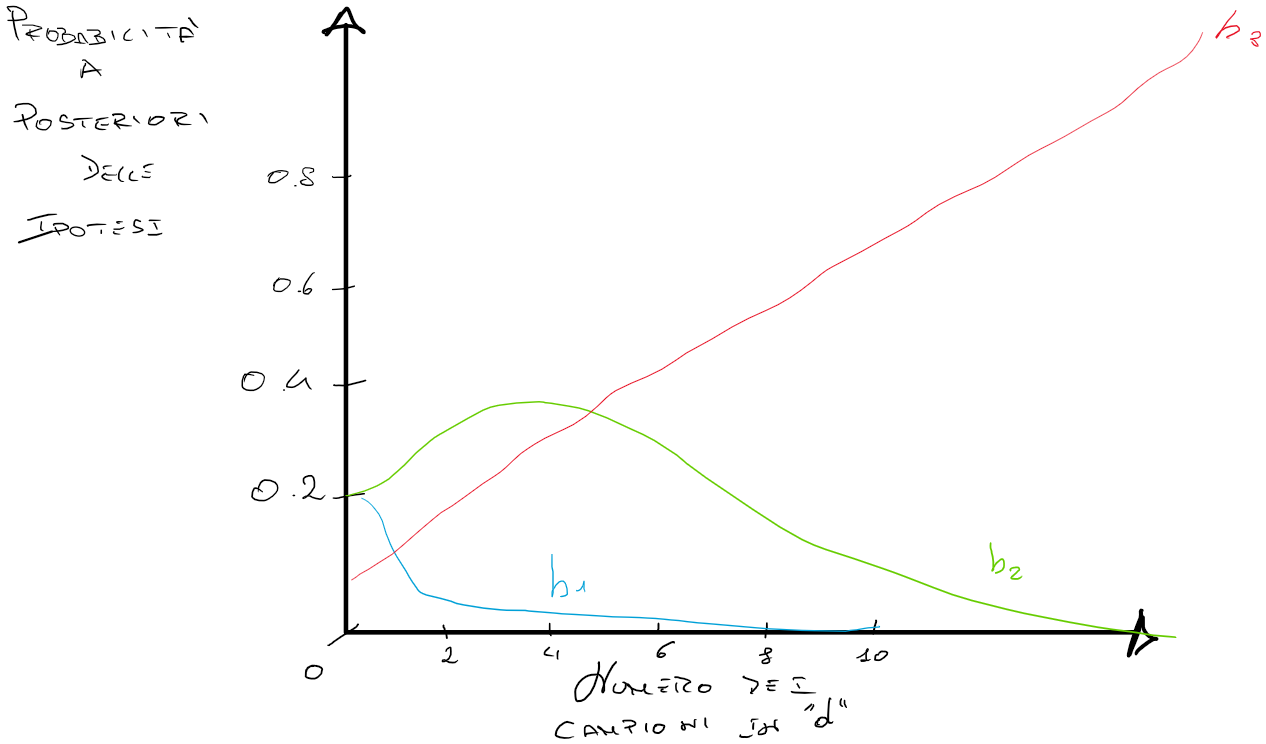
\includegraphics[width=1\textwidth]{img/prob1.png}
    \caption{Predizione delle ipotesi al variare dei campioni correttamente predetti.}
    \label{fig:Prob1}
\end{figure}
\subsection{Massima a posteriori}
La predizione bayesiana è \textbf{ottima}, indipendentemente dalle dimensioni dell'insieme dei dati: in altre parole, sarà corretta più spesso di qualsiasi altra predizione. Naturalmente c'è un prezzo da pagare per l'ottimalità dell'apprendimento bayesiano. Difatti nei sistemi reali i dati da gestire sono molti e spesso si deve ricorrere forzatamente ad una qualche forma ti approssimazione. \\ 
Un'approssimazione molto comune è formulare predizioni che si basano su un'ipotesi più probabile: la $h_i$ che massimizza $P(h_i| d)$. Questa viene spesso denominata \textbf{massimo a posteriori} o MAP. Le predizioni che si basano su un'ipotesi $h_{MAP}$ sono approssimativamente bayesiane dal momento che:
\[P(X|d) \approx P(X|h_{MAP})\]
La figura \ref{fig:Prob1} mostra difatti che l'ipotesi $h_2 = h_{MAP}$ dopo un certo numero di classificazioni tali per cui $d_{n+1} = x_k$ (ovvero dopo aver predetto una certa sequenza di classificazioni), per cui un agente MAP predirà che l'\textit{n-esimo} valore sarà opportunamente classificato con $x_k$ con probabilità 1. 
Man mano che vengono elaborati nuovi dati, la predizione MAP e quella bayesiana si avvicinano (dato che le altre predizioni "candidate" MAP diventano meno probabili). Generalmente trovare l'ipotesi MAP è più facile poiché si sta risolvendo un problema di ottimizzazione anziché eseguire una grande sommatoria.
\begin{definizione}
  Definiamo le \textit{ipotesi maximum a posteriori (MAP)} ogni ipotesi
  massimamente probabile:
  \[h_{MAP}=\operatorname*{argmax}_{h\in H}P(h|d)\]
  \[\operatorname*{argmax}_{h\in H}\frac{P(d|h)P(h)}{P(d)}\]
  Ma $P(d)$ può essere cancellato in quanto costante e indipendente da $h$,
  ottenendo:
  \[h_{MAP}=\operatorname*{argmax}_{h\in H}P(d|h)P(h)\]
\end{definizione}
\subsection{Massima Verosimiglianza}
Un'ultima semplificazione si può ottenere presupponendo una distribuzione a priori uniforme dello spazio delle ipotesi. Spesso si assume anche che ogni ipotesi è, a priori, equiprobabile e quindi possiamo semplificare i conti. La massima verosimiglianza (maximum likehood) si indica con ML. Esso è un approccio ragionevole quando non c'è ragione di preferire a priori un'ipotesi all'altra.
\begin{definizione}
  Dato che $P(d|h)$ viene spesso chiamata \textbf{likehood
    (\textit{probabilità})} di $D$ data $h$ viene definita \textbf{ipotesi
    maximum likehood (ML)} ogni ipotesi che massimizza $P(d|h)$:
  \[h_{ML}=\operatorname*{argmax}_{h\in H}P(d|h)\]
  potendo quindi trascurare $P(h)$ in quanto equivalente $\forall\, h\in H$
\end{definizione}
\subsubsection{Learn a Read-Value Function}
Ipotizziamo di voler trovare un'ipotesi per una funzione target:
\begin{figure}[H]
    \centering
    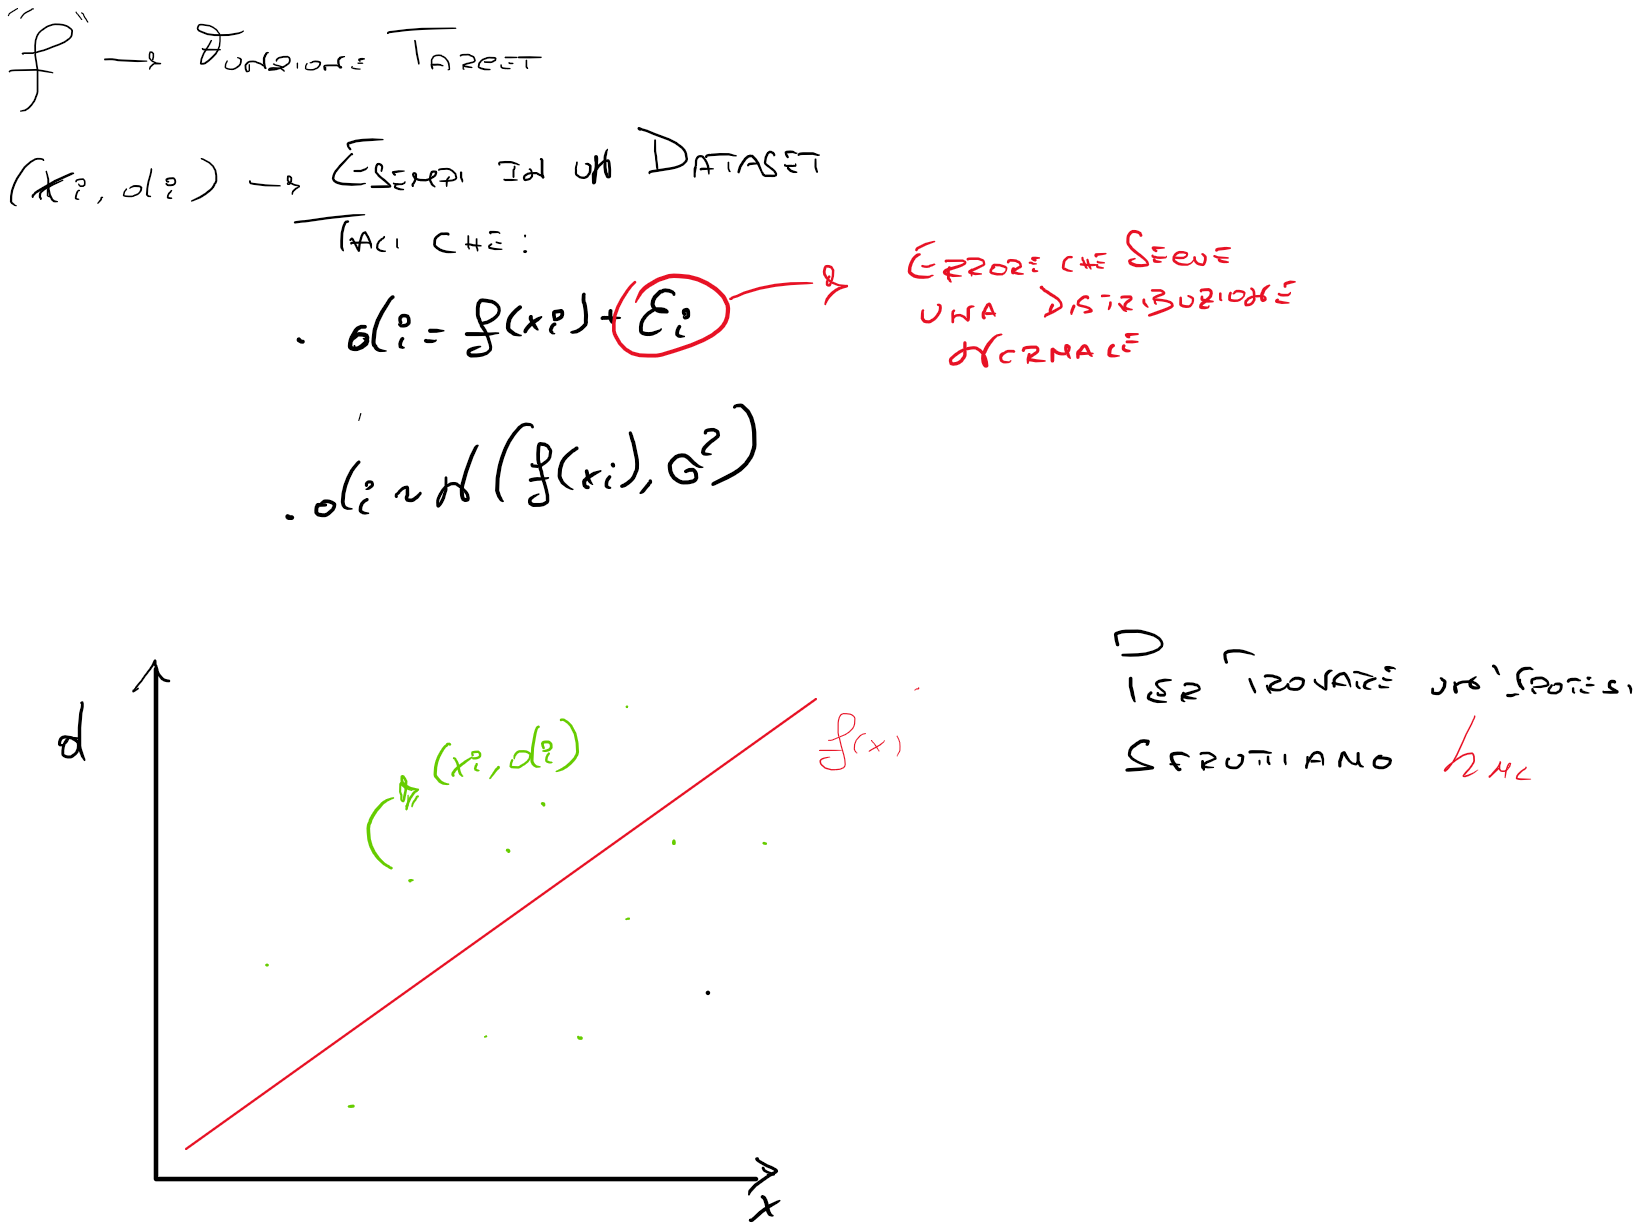
\includegraphics[width=1\textwidth]{img/hml.png}
\end{figure}
Avendo quindi che $h_{ML}=\operatorname*{argmax}_{h\in H}P(d|h)$ e che gli
eventi di training vengono assunti come indipendenti si ha che:
\[h_{ML}=\operatorname*{argmax}_{h\in H}\prod_{i=1}^mP(d_i|h) = \operatorname*{argmax}_{h\in H}P(d|h) \]
Dato quindi l'errore e$_i$ distribuito normalmente con media zero e varianza
sconosciuta $\sigma^2$ si ha che anche ogni $d_i$ segue la stessa
distribuzione attorno al target $f(x_i)$. Poiché stiamo scrivendo l'espressione
per $P(d|h)$, assumiamo che $h$ sia la descrizione corretta per $f$, quindi:
\[\mu=f(x_i)=h(x_i)\]
e avendo quindi, per la distribuzione normale:
\[h_{ML}=\operatorname*{argmax}_{h\in H}
  \prod_{i=1}^m\frac{1}{\sqrt{2\pi\sigma^2}}
  e^{-\frac{1}{2\sigma^2}(d_i-h(x_i))^2}\]
È comune massimizzare il logaritmo meno complicato, a causa della monotonia di
questa funzione, avendo:
\[h_{ML}=\operatorname*{argmax}_{h\in
    H}\prod_{i=1}^m\frac{1}{\sqrt{2\pi\sigma^2}}
  -\frac{1}{2\sigma^2}(d_i-h(x_i))^2\]
ma il primo termine è costante e indipendente da $h$ e quindi può essere
cancellato:
\[h_{ML}=\operatorname*{argmax}_{h\in
    H}\prod_{i=1}^m -\frac{1}{2\sigma^2}(d_i-h(x_i))^2\]
Sapendo che massimizzare questo termine negativo equivale a ridurre al minimo il
termine positivo corrispondente:
\[h_{ML}=\operatorname*{argmin}_{h\in
    H}\prod_{i=1}^m \frac{1}{2\sigma^2}(d_i-h(x_i))^2\]
e avendo che anche tutte le costanti sono indipendenti da $h$ e quindi possono
essere rimosse:
\[h_{ML}=\operatorname*{argmin}_{h\in H}\prod_{i=1}^m (d_i-h(x_i))^2\]
trovando che $h_{ML}$ è ciò che minimizza gli errori quadratici. \\
Si specifica la scelta della normale in quanto:
\begin{itemize}
  \item buona approssimazione di molti tipi di rumore nei sistemi fisici 
  \item il definizione del Limite Centrale mostra che la somma di un numero
  sufficientemente grande di variabili casuali indipendenti e identicamente
  distribuite obbedisce a una distribuzione Normale 
\end{itemize}
\textbf{\textit{Si considera solo il rumore sul valore del target e non sugli
    attributi che descrivono le istanze stesse}}.
% \subsection{Brute-Force MAP LEARNING}
% Si può usare il definizione di Bayes per specificare un algoritmo di apprendimento
% molto semplice detto \textbf{algoritmo Brute-Force MAP LEARNING} che si articola
% in 2 step:
% \begin{enumerate}
%   \item $\forall\, h\in H$ calcolo la probabilità a posteriori tramite il definizione
%   di Bayes:
%   \[P(h|d)=\frac{P(d|h)P(h)}{P(d)}\]
  
%   \item restituisco l'ipotesi $h_{MAP}$ con la più alta probabilità a
%   posteriori:
%   \[h_{MAP}=\operatorname*{argmax}_{h\in H}P(h|d)\]
% \end{enumerate}
% Però, per specificare il problema d'apprendimento per l'algoritmo, bisogna
% obbligatoriamente specificare i valori di:
% \begin{itemize}
%   \item $P(h)$
%   \item $P(d|h)$
% \end{itemize}
% e quindi dobbiamo obbligatoriamente fare una serie di assunzioni:
% \begin{itemize}
%   \item il training set deve essere privo di rumore, avendo:
%   \[d_i=c(x_i)\]
%   \item il target concept deve essere contenuto nello spazio delle ipotesi:
%   \[\exists h\in H \mbox{t.c. }h(x)=c(x),\,\,\,\forall\, x\in X\]
%   \item devo assumere che le ipotesi siano equiprobabili e quindi:
%   \[P(h)=\frac{1}{|H|}\,\,\,\forall\, h\in H\]
%   e avendo quindi:
%   \[P(d|h)=
%     \begin{cases}
%       1&\mbox{se } d_i=h(x_i),\,\,\,\forall\, d_i\in D\\
%       0&\mbox{altrimenti}
%     \end{cases}
%   \]
% \end{itemize}
% Si ha quindi che il problema di apprendimento per l'algoritmo è completamente
% definito. Possiamo quindi specificare che, nel primo step, ovvero quando si
% cerca $P(h|d)$, posso avere due casi:
% \begin{enumerate}
%   \item $h$ è inconsistente con $D$, avendo quindi:
%   \[P(h|d)=\frac{0\cdot P(h)}{P(d)}=0\]
%   \item $h$ è consistente con $D$, avendo quindi:
%   \[P(h|d)=\frac{1\cdot \frac{1}{|H|}}{P(d)}=\frac{1\cdot
%       \frac{1}{|H|}}{\frac{|VS_{H, D}|}{|H|}}=\frac{1}{|VS_{H, D}|}\] 
% \end{enumerate}
% Si ha quindi che questa analisi implica che, sotto le condizioni sopra definite,
% ogni ipotesi coerente è un'ipotesi MAP, perché per ogni ipotesi coerente si ha
% che:
% \[P(h|d)=\frac{1}{|VS_{H, D}|}\]
% \begin{figure}
%   \centering
%   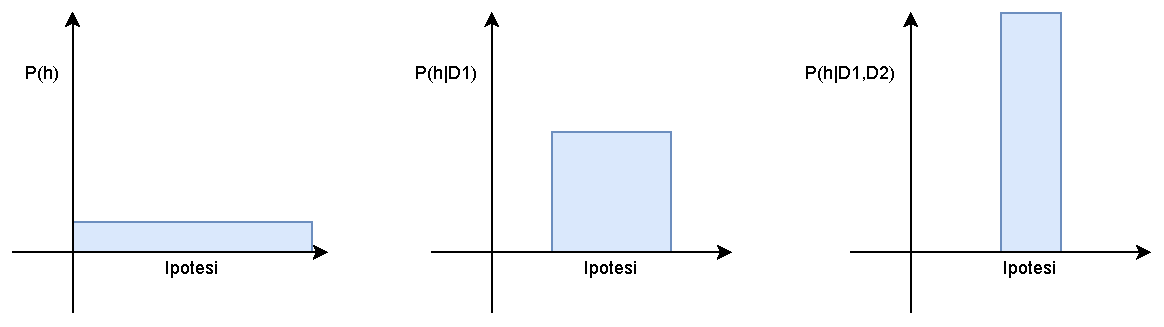
\includegraphics[scale = 0.6]{img/map.pdf}
%   \caption{Nell'immagine le evoluzioni di probabilità delle
%     ipotesi. Nel primo grafico tutte le ipotesi hanno la stessa probabilità, è
%     il punto di partenza. Con gli altri due grafici si ha che man mano che i
%     dati di addestramento si accumulano, la probabilità a posteriori delle
%     ipotesi inconsistenti diventa zero mentre la probabilità totale che si somma
%     a 1 è condivisa equamente tra le ipotesi consistenti rimanenti.}
% \end{figure}
% Si ha che ogni learner consistente ha in output ipotesi MAP se si assume a
% priori la distribuzione uniforme delle probabilità su $H$ dati di training
% deterministici e privi di rumore.\\
% Riprendendo per esempio anche l'algoritmo find-S si ha che:
% \begin{itemize}
%   \item ha in output ipotesi consistenti e quindi ipotesi MAP sotto la
%   distribuzione di probabilità $P(h)$ e $P(d|h)$
%   \item $\forall\, P(h)$ che favorisce le ipotesi più specifiche find-S trova
%   appunto le ipotesi MAP
% \end{itemize}
% A riprova che il metodo Bayesiano è un modo per caratterizzare il comportamento
% degli algoritmi di apprendimento.\\
% inoltre, identificando $P(h)$ e $P(d|h)$ base alle quali l'output è l'ipotesi
% ottimale, è possibile caratterizzare le ipotesi implicite dell'algoritmo ovvero
% il \textbf{bias induttivo} dell'algoritmo (avendo anche che l'inferenza
% induttiva è modellata da un sistema di ragionamento probabilistico equivalente
% basato sulla definizione di Bayes). \\
% Si introduce ora il problema di apprendere funzioni target a valori continui
% (reti neurali regressione lineare etc$\ldots$). Si ha che in base a determinate
% ipotesi, qualsiasi algoritmo di apprendimento che minimizzi l'errore quadratico
% tra l'ipotesi di output e i dati di addestramento, produrrà un'ipotesi
% ML. Prepariamo quindi il nostro insieme di assunzioni per il problema:
% \begin{itemize}
%   \item $h:X\to\mathbb{R},\,\,\,\forall\, h\in H$
%   \item li esempi sono della forma $\langle x_i, d_i\rangle$
%   \item la funzione target è definita come $f:X\to\mathbb{R}$
%   \item si hanno $m$ esempi di training dove il valore target di ogni esempio è
%   ``sporcato'' dal rumore casuale $e_i$ secondo una distribuzione di probabilità
%   normale con media nulla, avendo $d_i=f(x_i)+e_i$
% \end{itemize}
\subsection{Minima Lunghezza della descrizione}
Sia nell'apprendimento bayesiano che in quello MAP la distribuzione a priori delle ipotesi $P(h_i)$ ha un ruolo importante difatti ha il ruolo di \textit{penalizzare la complessità} nel caso di \textbf{overfitting}. Tipicamente le ipotesi più complesse hanno una probabilità a priori più bassa, sebbene abbiano una maggior capacità di adattarsi ai dati. Quindi la probabilità a priori rappresenta un compromesso tra la sua complessità e la sua capacità di adattarsi ai dati.
Anche in questo caso si usa il Rasoio di Occam, scegliendo di usare il principio
\textbf{Minimum Description Length (\textit{MDL})}, scegliendo la spiegazione
più breve per i dati osservati.\\
Tramite MDL posso ``giustificare'' la scelta di $h_{MAP}$ in base alla teoria
dell'informazione, infatti:
\[h_{MAP}=\operatorname*{argmax}_{h\in H}P(d|h)P(h)\]
\[=\operatorname*{argmax}_{h\in H}\log_2P(d|h)+\log_2P(h)\]
\[=\operatorname*{argmin}_{h\in H}-\log_2P(d|h)-\log_2P(h)\]
e queste equazioni possono essere interpretate come un'affermazione che sono
preferite ipotesi brevi, assumendo un particolare schema di rappresentazione per
la codifica d'ipotesi e dati.\\
Il principio MDL fornisce un modo per scambiare la complessità delle ipotesi
per il numero di errori commessi dall'ipotesi.\\

\textbf{Su slide altre informazioni su teoria dell'informazione.}
\section{Classificatore Bayesiano ottimo}
Ci si chiede quindi qual è la \textbf{classificazione più probabile} della nuova istanza
secondo i dati di training.\\
Vediamo con un esempio che non basta applicare $h_{MAP}$:
\begin{esempio}
  Sia $H=\{h_1, h_2, h_3\}$ con $P(h_1)=0.4$ e $P(h_2)=P(h_3)=0.3$.\\
  Si ha quindi che:
  \[h_{MAP}=h_1\]
  Consideriamo però una nuova istanza $x$ classificata positiva per $h_1$ e
  negativa per le altre due. Si ha quindi che:
  \begin{itemize}
    \item la probabilità che $x$ sia positivo è 0.4
    \item la probabilità che $x$ sia negativo è 0.6
  \end{itemize}
  e quindi la classificazione più probabile non è quella di $h_{MAP}$.
\end{esempio}
Abbiamo che la classificazione più probabile si ottiene combinando le previsioni
di tutte le ipotesi, ponderate in base alle loro probabilità posteriori. Data
$P(X|d)$ come la probabilità che la classificazione corretta sia $X$:
\[P(X|d)=\sum_{h_i\in H}P(X|h_i)P(h_i|d)\]
ottenendo che il classificatore Bayesiano ottimo è:
\[\operatorname*{argmax}_{X\in V}\sum_{h_i\in H}P(X|h_i)P(h_i|d)\]
dato $V$ come insieme di tutte le possibili predizioni esistenti.
\begin{esempio}
  Vediamo un esempio chiarificatore.\\
  Sia $V=\{+,-\}$ e siano:
  \begin{itemize}
    \item $P(h_1, d) =0.4,\,\,\, P(-, h_1) = 0,\,\,\, P(+, h_1) = 1$
    \item $P(h_2, d) =0.3,\,\,\, P(-, h_2) = 1,\,\,\, P(+, h2) = 0$
    \item $P(h_3, d) =0.3,\,\,\, P(-, h_3) = 1,\,\,\, P(+, h3) = 0$
  \end{itemize}
  Si hanno:
  \[\sum_{h_i\in H}P(+|h_i)P(h_i|d)=0.4\]
  \[\sum_{h_i\in H}P(-|h_i)P(h_i|d)=0.6\]
  \[\operatorname*{argmax}_{X\in \{+,-\}}\sum_{h_i\in H}P(X|h_i)P(h_i|d)= - \]
\end{esempio}
\section{Classificatore Bayesiano naive}
Il modello di rete bayesiana più usato nell'apprendimento automatico è probabilmente quello  \textbf{bayesiano ingenuo/naive}. Tale nomenclatura è data poiché il modello presume che gli attributi siano tutti condizionalmente indipendenti l'uno dall'altro, data la classe.
Il Classificatore Bayesiano naive si applica alle attività di learning in
cui ogni istanza $x$ è descritta da una giunzione di valori di attributi e in
cui la funzione target $f(x)$ può prendere un valore qualsiasi dall'insieme
finito $V$. Descriviamo gli esempi di training come $\langle d_1, d_2,\ldots
d_n\rangle $. \\
Applicando il metodo Bayesiano si ha:
\[h_{MAP}=\operatorname*{argmax}_{h\in V}P(h|d_1, d_2,\ldots d_n)\]
\[=\operatorname*{argmax}_{h\in V}\frac{P(d_1, d_2,\ldots d_n|h)P(h)}{P(d)}\]
e, rimuovendo le i fattori indipendenti:
\[h_{MAP}=\operatorname*{argmax}_{h\in V}P(d_1, d_2,\ldots d_n|h)P(h)\]
Avendo che:
\begin{itemize}
  \item $P(h)$ può essere stimato tramite la frequenza di $h$ in $D$
  \item $P(d_1, d_2,\ldots d_n|h)$ non può essere stimato in questo modo ma il
  numero di questi termini è pari a $|X|\cdot |V|$
\end{itemize}
Con il classificatore Bayesiano naive si hanno diverse semplificazioni. In primis
i valori degli attributi sono condizionatamente indipendenti:
\begin{itemize}
  \item $P(d_1, d_2,\ldots d_n|h)=\prod_iP(d_i|h)$
  \item il numero dei termini $d_1, d_2,\ldots d_n$ è pari a:
  \[|DA|\cdot |DT|+|DT|\]
  ove:
  \begin{itemize}
    \item $DA$ sta per attributi distinti/unici
    \item $DT$ sta per valori di target distinti/unici
  \end{itemize}
  \item non si ha la ricerca esplicita dentro $H$ ma solo il contro delle
  frequenze 
\end{itemize}
Si ha quindi il classificatore Bayesiano naive:
\[v_{NB}=\operatorname*{argmax}_{h\in V}P(h)\prod_iP(d_i|h)\]
\newpage
\begin{esempio}
  Vediamo un esempio chiarificatore.\\
  Sia dato il seguente dataset, con il target \textit{PlayTennis}:
  \begin{figure}[H]
    \centering
\    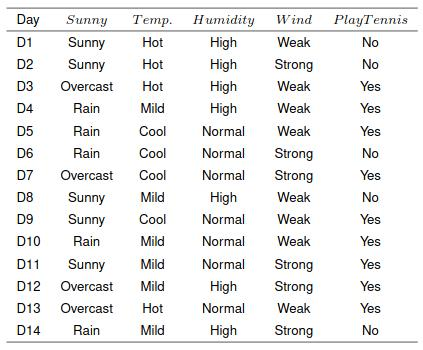
\includegraphics[scale = 0.7]{img/cbn.jpg}
  \end{figure}
  Si ha la nuova istanza:
  \[\langle Outlook=Sunny, Temperature=Cool, Humidity=High,
      Wind=Strong \rangle\]
  Si ha quindi che:
  \[\prod_iP(a_i|h)=(Outlook=sunny|h)\cdot
      P(Temperature=cool|h)\]\[\cdot P(Humidity=high|h)\cdot
      P(Wind=strong|h)\]
 
  Avendo la stima delle probabilità:
  \[P(PlayTennis=yes)=\frac{9}{14}=0.64\]
  \[P(PlayTennis=no)=\frac{5}{14}=0.36\]
  In modo analogo calcolo le probabilità condizionali. Per esempio per
  $Wing=Strong$:
  \[P(Wing=Strong|PlayTennis=yes)=\frac{3}{9}=0.33\]
  \[P(Wing=Strong|PlayTennis=no)=\frac{3}{5}=0.60\]
  Posso quindi calcolare $v_{NB}$:
  \[P(yes)\cdot P(Sunny|yes)\cdot P(cool|yes)\cdot P(high|yes)\cdot
    P(cool|yes)=0.0053\]
  \[P(no)\cdot P(Sunny|no)\cdot P(cool|no)\cdot P(high|no)\cdot
    P(cool|no)=0.0206\]
  Quindi si ha che:
  \[v_{NB}=no\]
  e normalizzando:
  \[\frac{0.0206}{0.0206+0.0053}\]
\end{esempio}
Si è visto come, normalmente, le probabilità sono stimate dalla frazione di
volte in cui si osserva che l'evento si verifica sul numero totale di
opportunità $N$:
\[\frac{n_c}{N}\]
è spesso questo metodo fornisce una buona stima.\\
Si ha però un limite se $n_c$ è molto piccolo, avendo risultati errati con:
\begin{itemize}
  \item sottovalutazione delle probabilità a causa di un bias
  \item se addirittura $n_c$ è nullo esso ``dominerà'' sul classificatore
  Bayesiano 
\end{itemize}
Si introduce un nuovo approccio Bayesiano sfruttando il cosiddetto
\textbf{m-estimate}, ovvero: 
\[\frac{n_c+m\cdot p}{n+m}\]
dove $p$ è una stima precedente della probabilità che desideriamo determinare,
ed $m$ è una costante chiamata \textit{equivalent sample size} che determina
quanto sia importante il peso di $p$ rispetto ai dati osservati.\\
In assenza d'informazioni aggiuntive $p$ ha distribuzione uniforme quindi si
ha, per $k$ numero di possibili valori di attributo:
\[p=\frac{1}{k}\]
Si nota che per $m$ nullo si ha che l'm-estimate è uguale a:
\[\frac{n_c}{n}\]
e quindi $m$ può essere interpretato come il numero di campioni virtuali
distribuiti su $p$ a cui vengono aggiunti gli $n$ esempi effettivi osservati.
\section{Esempi}
Si ricorda che si cerca una strategia per trovare la miglior ipotesi nello
spazio delle ipotesi. In questo caso si parla di ``migliore'' in termini di più
``probabile''. \\
Quando si fa inferenza bayesiana è tutto governato da \textit{incertezza} ma
permette di sfruttare conoscenze a priori.\\
Ricordiamo quindi la formula di Bayes:
\[P(h|d)=\frac{P(d|h)P(h)}{P(d)}\]
con:
\begin{itemize}
  \item $D$ è il dataset
  \item $h$ che per noi è l'ipotesi
  \item $P(h|d)$ che è la distribuzione a posteriori
  \item $P(h)$ è la distribuzione a priori
  \item $P(d|h)$ è la verosimiglianza
  \item $P(d)$ è l'evidenza
\end{itemize}
Sapendo che:
\[P(d)=\sum_i(d, h_i)=\sum_i P(d|h_i)P(h_i)\]
$P(d)$ è invariante rispetto al valore dell'ipotesi e quindi possiamo benissimo
rimuoverlo nel calcolo in quanto non influisce sulla probabilità a posteriori:
\[P(h_i|d)\varpropto P(d|h_i)P(h_i)\]
\begin{nota}
    Si ricorda che $\varpropto$ indica "\textit{proposizionale a}" quindi che due
cose sono uguali al più di una costante.
\end{nota}
Ricordiamo inoltre che la massima ipotesi a posteriori è:
\[h_{MAP}=\operatorname*{argmax}_{h\in H}P(h|d)=
  \operatorname*{argmax}_{h\in H}P(d|h)P(h)\]
Se si sa che anche la conoscenza a priori è ininfluente, essendo distribuita
seconda una distribuzione uniforme, e si parla d'ipotesi di massima
verosimiglianza:
\[h_{ML}=\operatorname*{argmax}_{h\in H}P(d|h)\]
L'approccio di Bayes nel machine learning è abbastanza oneroso, dovendo
calcolare tutte le probabilità a posteriori di ogni ipotesi (se $H$ è grande
diventa molto costoso).
\begin{esercizio}
  Si assuma di avere:
  \begin{table}[H]
    \centering
    \begin{tabular}{c||c|c|c|c}
      temp & $h_1$ & $h_2$ & $h_3$ & $h_4$\\
      \hline
      \hline
      hot & no & no & yes & yes\\
      cold & no &yes & no & yes \\
      \hline
      \hline
      $P(d|h)$ & 0 & 0 & 1 &0
    \end{tabular}
  \end{table}
  Si calcoli $h_{MAP}$, assumendo una conoscenza a priori con distribuzione
  uniforme su tutto lo spazio $H$.\\
  Si hanno quindi 4 ipotesi, ciascuna che esprime il valore dei due attributi
  $hot $ e $cold$. L'ultima riga ci dice anche la verosimiglianza di ogni
  ipotesi.\\
  Faccio quindi i conti, sapendo che ogni $P(h_i)=\frac{1}{4}$, avendo
  distribuzione uniforme per tutte le ipotesi.\\
  Calcolo innanzitutto:
  %14
  \[P(d)=\sum_i(d, h_i)=\sum_i
    P(d|h_i)P(h_i)=0\cdot\frac{1}{4}+0\cdot\frac{1}{4}+
    1\cdot\frac{1}{4}+0\cdot\frac{1}{4}=\frac{1}{4}\]
  
  e quindi:
  \[P(h_0|d)=\frac{P(d|h_0)P(h_0)}{P(d)}=
    \frac{0\cdot\frac{1}{4}}{\frac{1}{4}}=0\]
  \[P(h_1|d)=\frac{P(d|h_1)P(h_1)}{P(d)}=
    \frac{0\cdot\frac{1}{4}}{\frac{1}{4}}=0\]
  \[P(h_2|d)=\frac{P(d|h_2)P(h_2)}{P(d)}=
    \frac{1\cdot\frac{1}{4}}{\frac{1}{4}}=1\]
  \[P(h_3|d)=\frac{P(d|h_3)P(h_3)}{P(d)}=
    \frac{0\cdot\frac{1}{4}}{\frac{1}{4}}=0\]
  Si ottiene infine:
  \[h_{MAP}=1\]
\end{esercizio}
\begin{esercizio}
  Si consideri un problema di diagnostica medica con due ipotesi alternative:
  \begin{enumerate}
    \item il paziente ha il raffreddore (indichiamo la cosa con $raffreddore$)
    \item il paziente non ha il raffreddore (indichiamo la cosa con $\neg raffreddore$)
  \end{enumerate}
  Si hanno inoltre due possibili outcome per i dati dei laboratori:
  \begin{itemize}
    \item positivi, indicati con ``+'' (che indica se si pensa che si abbia il
    raffreddore)
    \item negativi, indicati con ``-'' (che indica se si pensa che non si abbia
    il raffreddore)
  \end{itemize}
  Abbiamo quindi le seguenti probabilità:
  \begin{itemize}
    \item $P(raffreddore)=0.008$
    \item $P(\neg raffreddore)=0.992$
    \item $P(test=+|raffreddore)=0.98$
    \item $P(test=-|raffreddore)=0.02$
    \item $P(test=+|\neg raffreddore)=0.03$
    \item $P(test=-|\neg raffreddore)=0.97$
  \end{itemize}
  Si supponga ora che un laboratorio studi un nuovo paziente e che ottenga un
  risultato positivo ``+'' e vediamo se possiamo dire se ha il raffreddore:
  \[P(raffreddore|test=+)\varpropto P(test=+|raffreddore)P(raffreddore)=0.0078\]
  \[P(\neg raffreddore|test=+)\varpropto P(test=+|\neg raffreddore)P(\neg raffreddore)=0.0298\]
  Quindi:
  \[h_{MAP}=\neg raffreddore\]
  Posso inoltre determinare la corretta probabilità normalizzando a 1:
  \[P(raffreddore|test=+)=\frac{0.0078}{0.0078+0.0298}=0.21\]
  \[P(\neg raffreddore|test=+)=\frac{0.0298}{0.0078+0.0298}=0.79\]
  Si nota quindi come il risultato dipenda molto dalla conoscenza a priori (che
  deve essere disponibile).
\end{esercizio}
\begin{esercizio}
  Si consideri la seguente tabella con un attributo e il target, entrambi
  booleani:
  \begin{table}[H]
    \centering
    \begin{tabular}{c||c}
      Temperature & Play Tennis\\
      \hline
      \hline
      H & yes\\
      H & yes\\
      H & no\\
      C & yes\\
      H & yes\\
      C & no\\
      C & no\\
      C & no\\
      C & yes\\
    \end{tabular}
  \end{table}
  Si hanno quindi vari calcoli:
  \begin{itemize}
    \item $P(H|yes)=0.6$
    \item $P(H|no)=0.25$
    \item $P(C|yes)=0.4$
    \item $P(C|no)=0.75$
    \item $P(yes)=0.56$
    \item $P(no)=0.44$
  \end{itemize}
  Si ha anche:
  \[P(H)=P(H|yes)P(yes)+P(H|no)P(no)=0.6\cdot 0.56+0.25\cdot 0.44 \]
  \[= 0.336+0.11=0.447\]
  \[P(C)=P(C|yes)P(yes)+P(C|no)P(no)=0.4\cdot 0.56+0.75\cdot 0.44 \]
  \[= 0.224+0.33=0.554\]
\end{esercizio}
Ricordiamo che per Naive Bayes si ha, avendo una sequenza $d_1, d_2\ldots d_n$ di
osservazioni: 
\[h_{MAP}=\operatorname*{argmax}_{h\in H}P(h|d_1, d_2\ldots d_n)\]
\[=\operatorname*{argmax}_{h\in H}\frac{P(d_1, d_2\ldots d_n|h)P(h)}{P(d)}\]
\[\varpropto\operatorname*{argmax}_{h\in H}P(d_1, d_2\ldots d_n|h)P(h)\]
Per semplificare, tramite naive Bayes, si può assumere:
\[P(d_1, d_2\ldots d_n|h)=\prod_iP(d_i|h)\]
ovvero indipendenza condizionata (dicendo che un valore $d:i$ è indipendente da
un qualunque $d_j$) e quindi si ha, sostituendo:
\[h_{MAP}=\operatorname*{argmax}_{h\in H}P(h)\prod_iP(d_i|h)\]
\newpage
\begin{esercizio}
  Dati 6 esempi con tre attributi e target $T$ (attributi e target sono
  booleani): 
  \begin{table}[H]
    \centering
    \begin{tabular}{c||c|c|c|c}
      Esempi & $A$ & $B$ & $C$ & $T$\\
      \hline
      \hline
      $x_1$ & 1 & 1 & 1 & 0\\
      $x_2$ & 0 & 1 & 1 & 0\\
      $x_3$ & 1 & 0 & 1 & 1\\
      $x_4$ & 0 & 0 & 0 & 1\\
      $x_5$ & 0 & 1 & 0 & 1\\
      $x_6$ & 1 & 1 & 0 & ?\\
    \end{tabular}
  \end{table}
  Si completi la tabella con la label $T$ per $x_6$.\\
  Dividiamo in:
  \begin{itemize}
    \item $h_0=[T=0]$
    \item $h_1=[T=1]$
  \end{itemize}
  Si ha quindi per la prima ipotesi ($h_0$), sempre pensando a $x_6$:
  \[P(T=0|A=1, B=1, C=0)=\frac{P(A=1, B=1, C=0|T=0)P(T=0)}{P(x_6)}\]
  elimino l'evidenza:
  \[\varpropto P(A=1, B=1, C=0|T=0)P(T=0)\]
  uso l'assunzione di Naive Bayes:
  \[\varpropto P(A=1|T=0)P(B=1|T=0)P(C=0|T=0)P(T=0)
    \varpropto \frac{1}{2}\cdot 1\cdot 0\cdot \frac{2}{5}\]
  Avendo quindi, svolgendo il conto:
  \[P(h_0|x_6)\varpropto  \frac{1}{2}\cdot 1\cdot  0\cdot\frac{2}{5}=0\]
  

  Si passa poi alla seconda ipotesi ($h_1$), sempre pensando a $x_6$:
  \[P(T=1|A=1, B=1, C=0)=\frac{P(A=1, B=1, C=0|T=1)P(T=1)}{P(x_6)}\]
  elimino l'evidenza:
  \[\varpropto P(A=1, B=1, C=0|T=1)P(T=1)\]
  uso l'assunzione di Naive Bayes:
  \[\varpropto P(A=1|T=1)P(B=1|T=1)P(C=0|T=1)P(T=1)
    \varpropto \frac{1}{3}\cdot \frac{1}{3}\cdot \frac{2}{3}\cdot\frac{3}{5}\]
  Avendo quindi, svolgendo il conto:
  \[P(h_1|x_6)\varpropto  \frac{1}{3}\cdot \frac{1}{3}\cdot
    \frac{2}{3}\cdot\frac{3}{5}=\frac{2}{45}\]
  So quindi che $h_{MAP}=h_1$, avendo che la probabilità con $h_1$ è maggiore di
  quella con $h_0$. Si ha quindi, avendo che per $x_6$ scelgo $h_1$ che
  corrisponde ad avere $T=1$:
  \begin{table}[H]
    \centering
    \begin{tabular}{c||c|c|c|c}
      Esempi & $A$ & $B$ & $C$ & $T$\\
      \hline
      \hline
      $x_1$ & 1 & 1 & 1 & 0\\
      $x_2$ & 0 & 1 & 1 & 0\\
      $x_3$ & 1 & 0 & 1 & 1\\
      $x_4$ & 0 & 0 & 0 & 1\\
      $x_5$ & 0 & 1 & 0 & 1\\
      $x_6$ & 1 & 1 & 0 & 1\\
    \end{tabular}
  \end{table}
  
  Si può anche calcolare, per completezza:
  \[P(x_6)=\sum_iP(x_6, h_i)=\sum_{i\in\{0, 1\}}P(A=1, B=1, C=0|T=i)P(T=i)\]
  \[= P(A=1|T=0)P(B=1|T=0)P(C=0|T=0)P(T=0)+\]
  \[P(A=1|T=1)P(B=1|T=1)P(C=0|T=1)P(T=1)\]
  \[=( \frac{1}{2}\cdot 1\cdot  0\cdot\frac{2}{5})+(\frac{1}{3}\cdot
    \frac{1}{3}\cdot \frac{2}{3}\cdot\frac{3}{5})\]
  \[=\frac{1}{3}\cdot \frac{1}{3}\cdot
    \frac{2}{3}\cdot\frac{3}{5}=\frac{2}{45}\]

  Posso quindi calcolare:
  \[P(h_1|x_6)=P(T=1|A=1, B=1, C=0)=\frac{P(A=1, B=1, C=0|T=1)P(T=1)}{p(x_6)}\]
  \[=\frac{P(A=1|T=1)P(B=1|T=1)P(C=0|T=1)P(T=1)}{p(x_6)}\]
  \[=\frac{\frac{1}{3}\cdot \frac{1}{3}\cdot
      \frac{2}{3}\cdot\frac{3}{5}}
    {\frac{1}{3}\cdot \frac{1}{3}\cdot
      \frac{2}{3}\cdot\frac{3}{5}}=1\]
  Ugualmente dovrei calcolare $P(h_0|x_6)$ ma sapendo che i valori sono booleani
  e quindi ho solo $h_1$ e $h_0$, avendo $P(h_1|x_6)=1$ so che
  $P(h_0|x_6)=0$. \\
  Si hanno quindi:
  \begin{itemize}
    \item $h_{MAP}=h_1:=[T=1]$
    \item $P(x_6)=\frac{1}{3}\cdot \frac{1}{3}\cdot
    \frac{2}{3}\cdot\frac{3}{5}=\frac{2}{45}=0.04$
    \item $P(x_6|T=0)P(T=0)= \frac{1}{2}\cdot 1\cdot  0\cdot\frac{2}{5}=0$
    \item $P(x_6|T=0)= \frac{1}{2}\cdot 1\cdot  0=0$
    \item $P(A=1|T=0)=\frac{2}{5}$
    \item $P(T=0)=\frac{2}{5}$
    \item $P(h_0|x_6)=P(T=0|x_6)=0$
    \item $P(x_6|T=1)P(T=1)=\frac{1}{3}\cdot \frac{1}{3}\cdot
    \frac{2}{3}\cdot\frac{3}{5}=\frac{2}{45}=0.04$
    \item $P(x_6|T=1)=\frac{1}{3}\cdot \frac{1}{3}\cdot
    \frac{2}{3}=\frac{2}{27}=0.07$
    \item $P(B=1|T=1)=\frac{1}{3}$
    \item $P(T=1)=\frac{3}{5}$
    \item $P(h_1|x_6)=P(T=1|x_6)=1$
  \end{itemize}
\end{esercizio}%6

%---------- Clustering ----- 
\chapter{Clustering}
\begin{figure}[H]
    \centering
    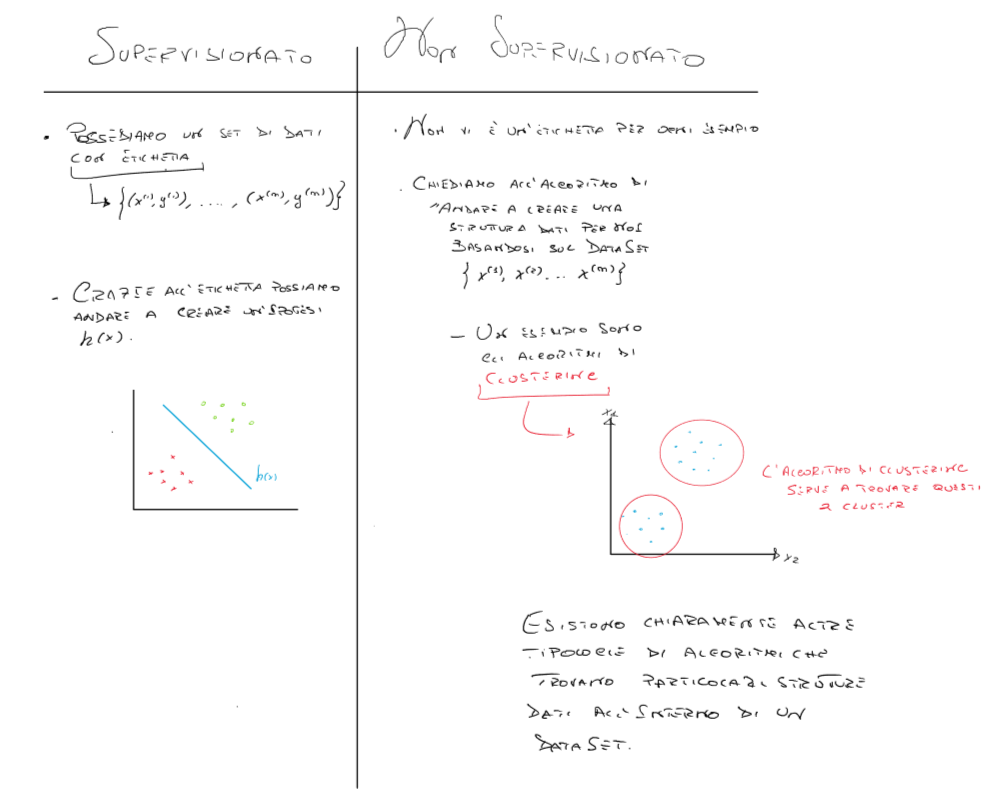
\includegraphics[width=1\textwidth]{img/LearningNonSupervisionato.png}
\end{figure}
Il \textbf{clustering} è un approccio non supervisionato. Come se stessimo
lavorando ``ad occhio'' si potrebbero avere vari criteri per effettuare il
raggruppamento delle istanze, in mancanza di label. Il criterio di scelta è
praticamente arbitrario e il termine ``classificare'' diventa più un
``raggruppare''. Il sistema è quindi flessibile nel decidere i criteri (che non
può essere scelto in base alle label) sfruttando concetti come la distribuzione
dei dati. I risultati ottenuti da un apprendimento
non supervisionato potrebbero ``sorprendere'' in quanto potrebbero essere
imprevedibili a priori. In ogni caso l'incertezza del clustering non è la sola,
in quanto anche un sistema supervisionato potrebbe comunque lasciare spazio ad
incertezza sulle ipotesi (non riuscendo magari ad avere tutte le label possibili
per l'insieme dei casi).\\ 
Possiamo pensare di rappresentare nello spazio (con dimensione pari al numero di
attributi delle istanze) le varie istanze per poi cercare di capire come
etichettare le varie istanze la cui etichetta non è nota. Si procede quindi
\textbf{raggruppando per distanza} (se è vicina a istanze con una certa
etichetta nota uguale anche istanza di cui cerchiamo l'etichetta avrà
quell'etichetta), usando la \textit{distanza di Hamming} o la \textit{distanza
  Euclidea}, ma prima di parlarne introduciamo meglio tutto il discorso. \\
La ``decisione forte'' è raggruppare e quindi scegliere in base alla distanza,
definendo prima la distanza stessa, misurando poi il risultato secondo un certo
criterio di misura (sempre basato sulla distanza).\\
Avendo una classificazione non supervisionata si ha una scarsa conoscenza a
priori dei dati da analizzare, puntando quindi all'estrazione automatica delle
classi mentre in quella supervisionata si partiva da classi etichettate, avendo
magari speso costo computazionale per ottenerle, e da una struttura
classificatoria conosciuta (avendo un set d'ipotesi possibili). I sistemi non
supervisionati tornano comodo quando la distribuzione dei valori degli attributi
è informazione sufficiente per separare le istanze in più classi, si hanno
quindi domini dove questo fattore è determinante. Con l'apprendimento non
supervisionato quindi la non conoscenza a priori è anche un vantaggio (magari le
etichette che uso nel supervisionato potrebbero essere errate), insieme
alla riduzione dell'errore umano. Un altro pro è che tutte le classi con
caratteristiche uniche vengono identificati e quindi i metodi di apprendimento
non supervisionato sono efficaci con elementi di tipo numerico, che diventano
coordinate in uno spazio, e con elementi dotati di ordinamento intrinseco, per
il calcolo delle distanze. Di contro le classi ottenute non per forza hanno un
significato. Inoltre l'utente ha poco controllo sulla procedura e sui risultati
e tali metodi sono meno efficaci con elementi ordinati in modo arbitrario o
parziale. \\
Si cerca quindi di separare un insieme di elementi in sottoinsiemi con elementi
accomunati da caratteristiche comuni, in base a uno o più attributi con la
scelta dell'attributo viene fatta dall'algoritmo di apprendimento. Tra i campi
d'intersse si hanno:
\begin{itemize}
  \item data mining
  \item pattern recognition
  \item image analysis 
  \item bioinformatica 
  \item ricerche di mercato
  \item pianificazione urbana 
  \item sismologia 
  \item astronomia
\end{itemize}
Ogni elemento da classificare viene specificato da un vettore caratteristico e
si ha una misura di similarità tra elementi. Si hanno quindi due criteri da 
rispettare:
\begin{itemize}
  \item \textbf{omogeneità} quando elementi dello stesso cluster hanno alto
  livello di similarità, quindi dentro il cluster
  \item \textbf{separazione} quando elementi di cluster diversi hanno basso
  livello di similarità, quindi tra cluster
\end{itemize}
\section{Definizioni Generali}
\begin{definizione}
  Dato $N=\{e_1,\ldots, e_n\}$ un insieme di $n$ elementi e sia
  $C=\{C_1,\ldots, C_k\}$ una partizione di $N$ in sottoinsiemi. Ogni $C_i$ è
  detto \textbf{cluster} e $C$ è detto \textbf{clustering} di $N$.
\end{definizione}
\begin{definizione}
  Dati due elementi di $N$ essi sono \textbf{mates} rispetto a $C$ se
  appartenenti allo stesso cluster $C_i$
\end{definizione}
Un elemento può essere rappresentato da un vettore di numeri reali, ciascuno dei
quali misura una specifica caratteristica (feature).\\
\begin{definizione}
  Definiamo la \textbf{misura di similarità} tramite la \textbf{distanza tra
    vettori}. Si hanno tre distanze:
  \begin{itemize}
    \item la \textbf{distanza euclidea} (che è la solita distanza ottenuta dal
    definizione di Pitagora, è semplicemente la lunghezza del segmento che collega
    due punti nello spazio):
    \[d(\vec{x},\vec{y})=\sqrt{\sum_i (x_i-y_i)^2} = \lVert x_i - y_i \rVert^2\]
    è invariante rispetto alle  traslazioni e rotazioni degli assi
    \item la \textbf{distanza di Manhattan} (misuro gli spostamenti, che hanno
    peso 1, tra due punti in termini di somma ti tali spostamenti che formano
    una linea spezzata):
    \[d(\vec{x},\vec{y})=\sum_i (x_i-y_i)\]
    Non è invariante rispetto a traslazioni o rotazioni degli assi e pone meno
    enfasi sulle variabili con distanze maggiori, non elevando al quadrato le
    differenze
    
    \item la \textbf{distanza di Minkowski} (dando un peso diverso rispetto alla
    distanza euclidea):
    \[d(\vec{x},\vec{y})=\sqrt[k]{\sum_i (x_i-y_i)^k}\]
    In altri termini questa è la forma generica, infatti al variare di $k$ si
    hanno le varie distanze:
    \begin{itemize}
      \item con $k=1$ ottengo la distanza di Manhattan
      \item con $k=2$ ottengo la distanza euclidea
      \item con $k=\infty$ ottengo la distanza di Lagrange-\v{C}eby\v{s}\"{e}v
    \end{itemize}
    Useremo soprattutto il caso euclideo.
  \end{itemize}
\end{definizione}
In generale si hanno varie tipologie di clustering, come da figura \ref{fig:clu}
in base all'approccio di studio delle istanze o di studio dei confini tra
cluster. Questo discorso non lo approfondiremo ma si ha:
\begin{itemize}
  \item \textbf{gerarchico} quando collocano gli elementi in input in una
  struttura gerarchica ad albero, in cui le distanze tra nodi riflettono le
  similarità degli elementi. Gli elementi sono localizzati sulle foglie
  dell’albero. Come pro si ha intuitività grazie a una struttura singola,
  coerente e globale. Si ha quindi:
  \begin{itemize}
    \item \textbf{Agglomerativi} quando bisogna scegliere la coppia di cluster da fondere
    \item \textbf{divisivi}, quando si deve determinare il cluster da dividere
  \end{itemize}
  Come algoritmi si hanno:
  \begin{itemize}
    \item Neighbor joining
    \item Metodo del centroid
  \end{itemize}
  \item \textbf{non gerarchico/partitivo} quando mirano a ripartire le $n$ unità
  della popolazione in $K$ gruppi, fornendo una sola partizione anziché una
  successione di partizioni tipica dei metodi gerarchici.\\
  Come algoritmo si ha, ad esempio, \textbf{K-means}
  definendo $K$ cluster tali per cui si abbiano punti vicini in cluster
  separati. È un algoritmo iterativo
\end{itemize}
\begin{figure}
  \centering
  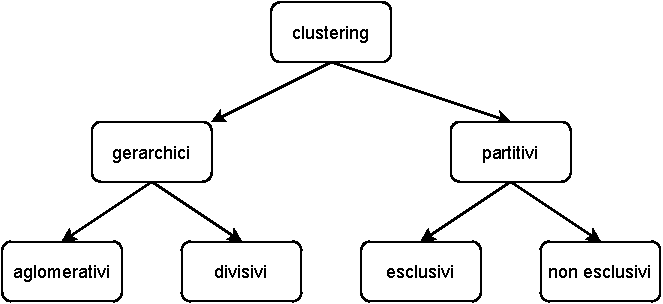
\includegraphics[scale = 1]{img/clu.pdf}
  \caption{Albero delle tipologie di clustering}
  \label{fig:clu}
\end{figure}
\section{K-Means}
\begin{definizione}
  definiamo \textbf{dendrogramma} come un albero (grafo) utilizzato per
  visualizzare la somiglianza nel processo di ``raggruppamento''.
  
\end{definizione}
Questi algoritmo è quello che vedremo per il metodo non approssimato. Si ha che
la  soluzione non è visualizzabile attraverso dendrogrammi e assume che il
numeor $K$ di cluster sia noto, puntando a minimizzare le distanze tra elementi
e i centroidi (un punto geometrico di riferimento per i cluster) dei clusters
loro assegnati.\\
L'algoritmo lavora con dati numerici in cinque step e si basa su due principali funzioni:
\begin{enumerate}
    \item \textbf{Assegnazione del Cluster}: ogni elemento viene assegnato ad un cluster mediante il centroide più vicino.
    \item \textbf{Movimento dei Centroidi}: i centroidi vengono spostati finché non viene rintracciati i cluster ottimi.
\end{enumerate}
\begin{enumerate}
  \item Si fissano randomicamente $K$ centroidi iniziali di altrettanti cluster
  \begin{figure}[H]
    \centering
    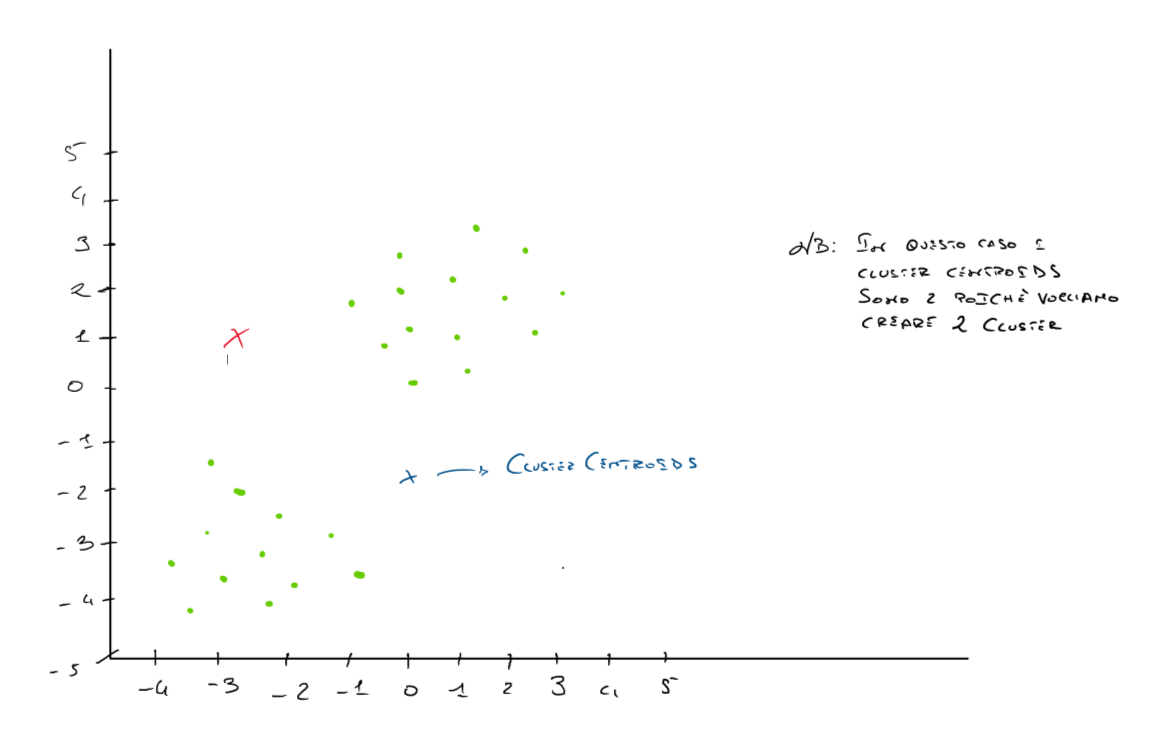
\includegraphics[width=1\textwidth]{img/kmeans1.PNG}
\end{figure}
  \item Per ogni elemento si calcola la distanza da ciascun centroide e lo si
  assegna al più vicino. L'assegnazione ad un centroide indica l'assegnazione al relativo cluster.
  \begin{figure}[H]
    \centering
    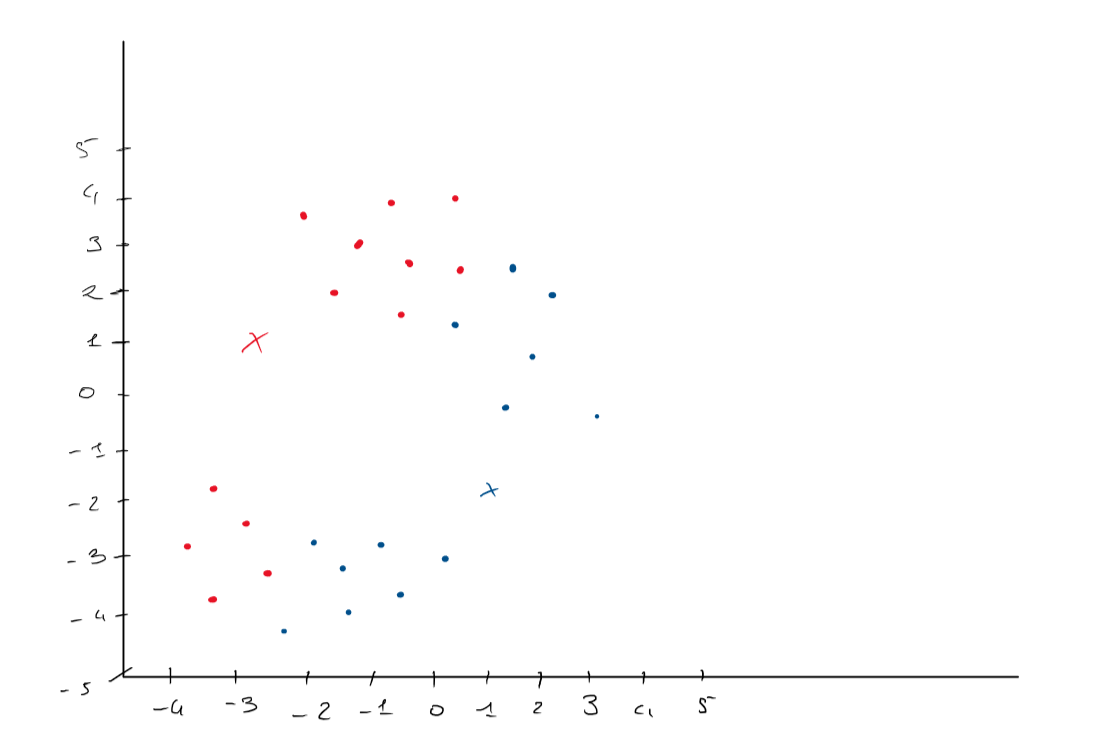
\includegraphics[width=1\textwidth]{img/kmeans2.PNG}
\end{figure}
    \begin{nota}
     Qualora $x^{(i)} \approx c^{(j)} \implies x^{(i)} \in Cluster_j$
    \end{nota}
  \item Per la partizione provvisoria così ottenuta si ricalcolano le posizioni dei centroidi per ogni cluster. Ciò avviene sfruttando la media aritmetica dei punti del cluster parziale. I centroidi vengono spostati in relazione alla media stessa.
  \begin{figure}[H]
    \centering
    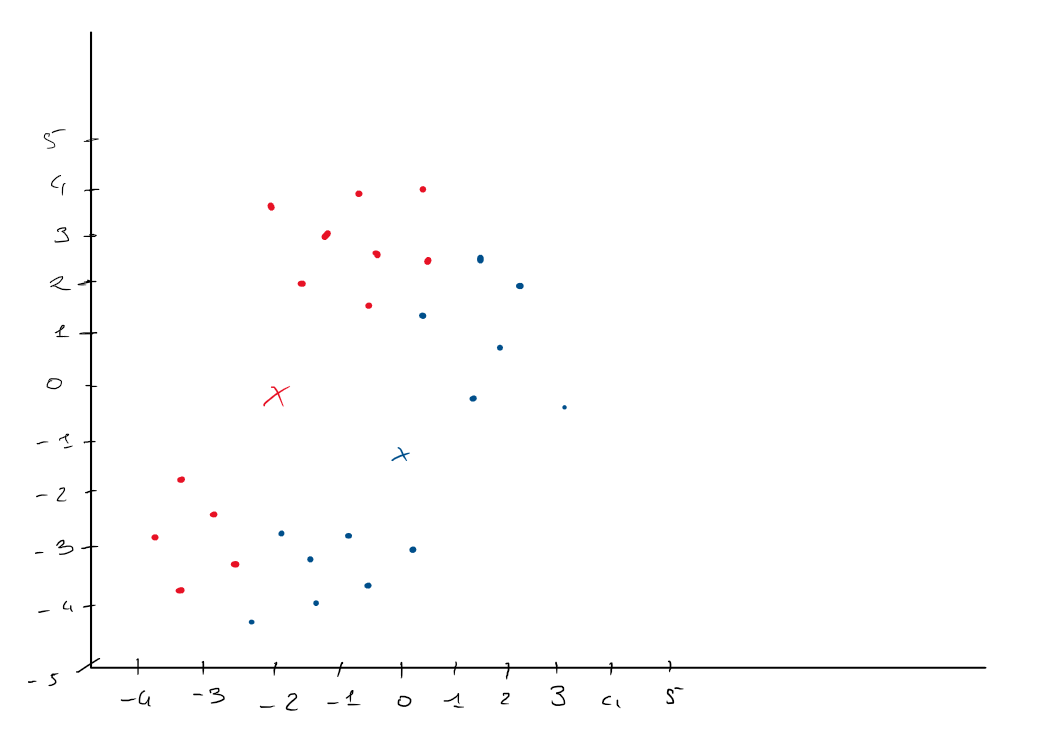
\includegraphics[width=1\textwidth]{img/kmeans3.PNG}
\end{figure}
  \item si ripetono le operazioni 3 e 4 finché Si raggiunge il numero massimo di
  iterazioni impostate, avendo un euristica, o non si verificano altri
  spostamenti, avendo una stabilità di risultato, avendo il risultato
  ``migliore'' 
      \begin{figure}[H]
    \centering
    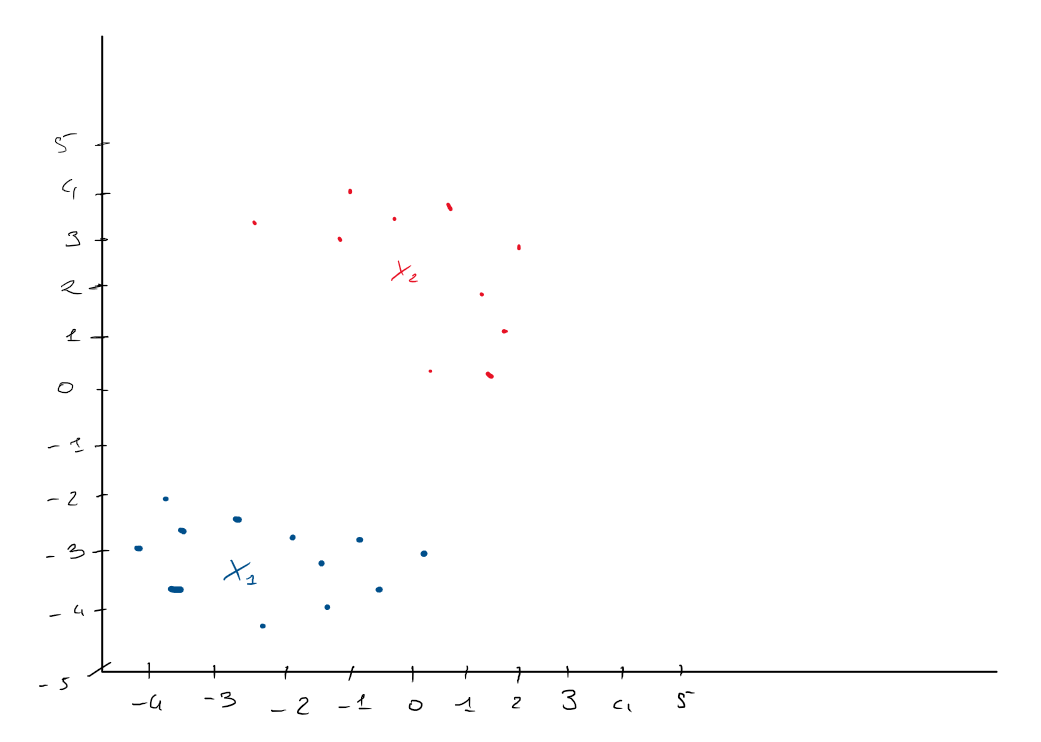
\includegraphics[width=1\textwidth]{img/kmeans4.PNG}
\end{figure}
%GIF
\begin{nota}
Gif animation: \url{https://machinelearningmedium.com/assets/2018-04-19-k-means-clustering/fig-1-clustering-animation.gif?raw=true}
\end{nota}
\end{enumerate}
Si nota quindi la semplicità d'implementazione e un tempo di calcolo in :
\[O(tKn)\]
con:
\begin{itemize}
  \item $n$ cardinalità dell'insieme dei dati
  \item $K$ numero di cluster
  \item $t$ numero d'iterazioni del ciclo (avendo quindi $kt<<n$)
\end{itemize}
\subsection{Algoritmo Formale}
Ipotizziamo che sia i centroidi $\mu$ che gli esempi $x$ siano \textbf{vettori}.
\textbf{Input:}
\begin{itemize}
    \item  $K$: numero di clusters
    \item $x^{(1)}, x^{(2)}, \cdots, x^{(m)}$: trainingset non supervisionato
\end{itemize}
\textbf{Algoritmo:}
\begin{itemize}
    \item $\mu_1, \mu_2, \cdots, \mu_k \in \mathbb{R}^n$: scelta randomica di centroidi.
\end{itemize}
% <![CDATA[
\begin{align*}
Repeat \{ \\
    \text{for }i &= 1\text{ to }m \text{ ---> Assegnazione del cluster}\\
        & c^{(i)} =\text{ indice (from }1\text{ to }K\text{) del centroide più vicino a }x^{(i)}\text{ -----> } min_k \lVert x^{(i)} - \mu_k \rVert^2 \\
    \text{for }k &= 1\text{ to }K \text{---> Movimento dei centroidi} \\
        & \mu_k =\text{ media dei punti assegnati al cluster }k\text{ -----> } \frac {\text{sum of } x^{(i)}\text{, where }c^{(i)} = k} {\text{number of }c^{(i)} = k} \\
\}
\end{align*} %]]>
Si noti che i due cicli for riguardano i due principali step da compiere. In particolare durante lo spostamento dei centroidi potrebbe accadere un esempio simile:
\begin{figure}[H]
    \centering
    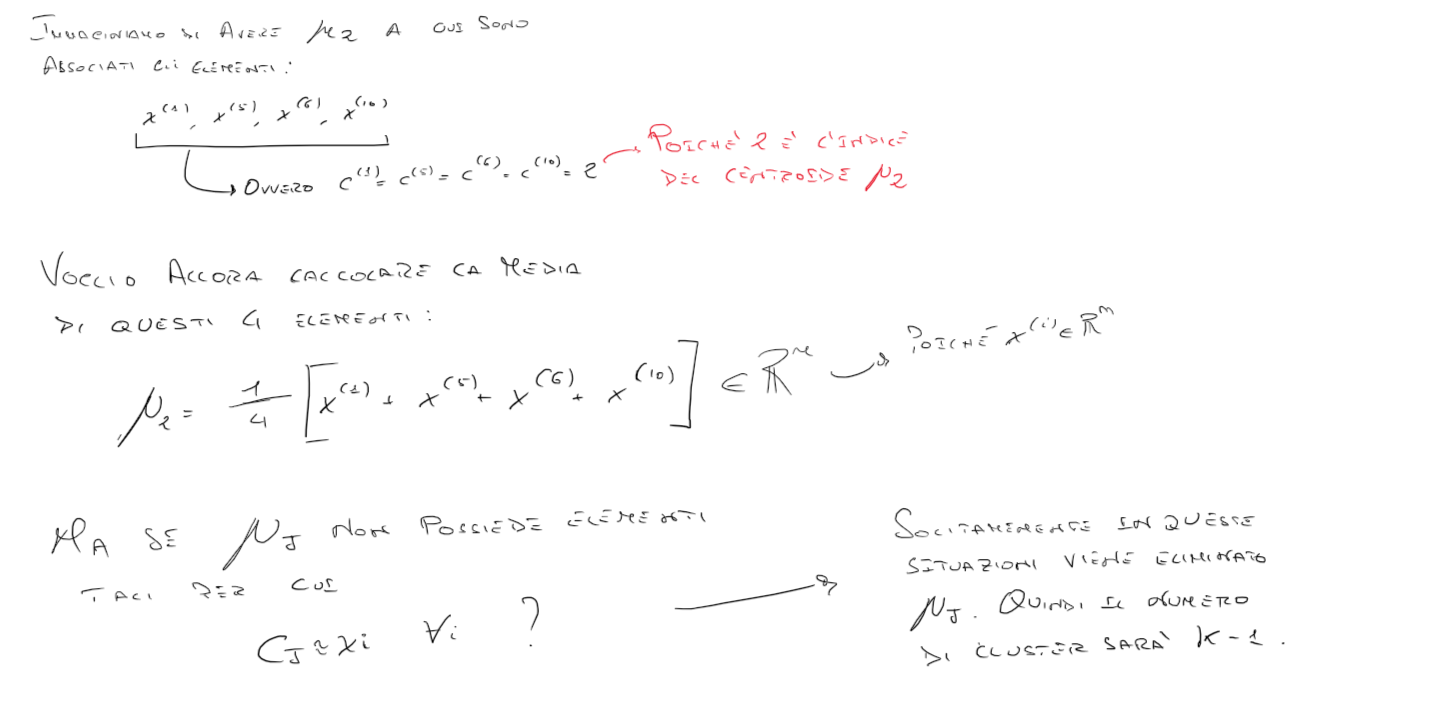
\includegraphics[width=1\textwidth]{img/kmeans16.PNG}
\end{figure}
\subsection{K-Means per clusters non separati}
Un altro problema è dato da dati distribuiti secondo diverse ``dimensioni''
nello spazio ma l'algoritmo lavorando sui centroidi potrebbe misclassificare
questo dettaglio, non distinguendo i corretti insiemi di punti. Analogamente
succede se si hanno insiemi di punti più o meno densi, portando a
misclassicazioni. Sempre in modo analogo le proprietà di distribuzione
geometrica degli elementi comporta problemi (anche con un $K$ adeguato).
Per superare queste difficoltà si può provare ad aumentare il numero di cluster,
unendo poi, in un secondo passaggio, i vari cluster secondo certi criteri,
magari avendo una netta separazione lineare tra cluster.
 \begin{figure}[H]
    \centering
    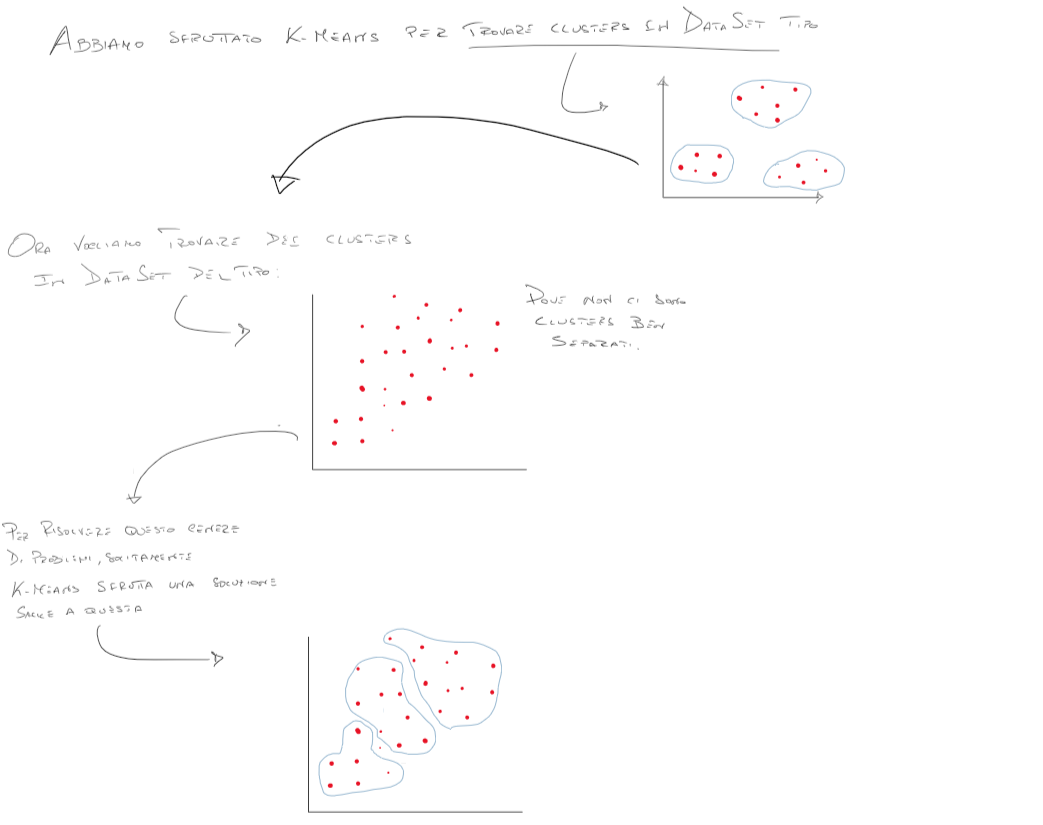
\includegraphics[width=1\textwidth]{img/kmeans5.PNG}
\end{figure}
\subsection{Optimization Objective}
\begin{definizione}
  Siano:
  \begin{itemize}
      \item $c^{(i)}$: l'\textbf{indice} del cluster a cui è assegnato l'esempio $x^{(i)}$. 
      \begin{nota}
      Gli indici dei clusters $c^{(i)}$ variano nell'insieme $1 \cdots K$.
      \end{nota}
      \item $\mu_k$ il centroide k-esimo.
      \item $\mu_{c^{(i)}}$ il centroide del cluster a cui è stato assegnato 'esempio $x^{(i)}$.
      \begin{nota}
      $x^{(5)} \in \mu_1 \implies c^{(5)} = 1$
      \end{nota}
  \end{itemize}
  Allora definiamo la funzione di costo (\textbf{funzione di distorsione}), come:
  \[J(c^{(1)}, c^{(2)}, \cdots, c^{(m)}, \mu_1, \mu_2, \cdots, \mu_K) = {1 \over m} \sum_{i=1}^m \lVert x^{(i)} - \mu_{c^{(i)}} \rVert^2\]
  Da cui si evince la funzione di ottimizzazione:
  \[min_{c^{(1)}, c^{(2)}, \cdots, c^{(m)},\\ \mu_1, \mu_2, \cdots, \mu_K} J(c^{(1)}, c^{(2)}, \cdots, c^{(m)}, \mu_1, \mu_2, \cdots, \mu_K)\]
\end{definizione}
\begin{nota}
$\lVert x^{(i)} - \mu_{c^{(i)}} \rVert^2$ è la distanza tra un esempio e un centroide.
 \begin{figure}[H]
    \centering
    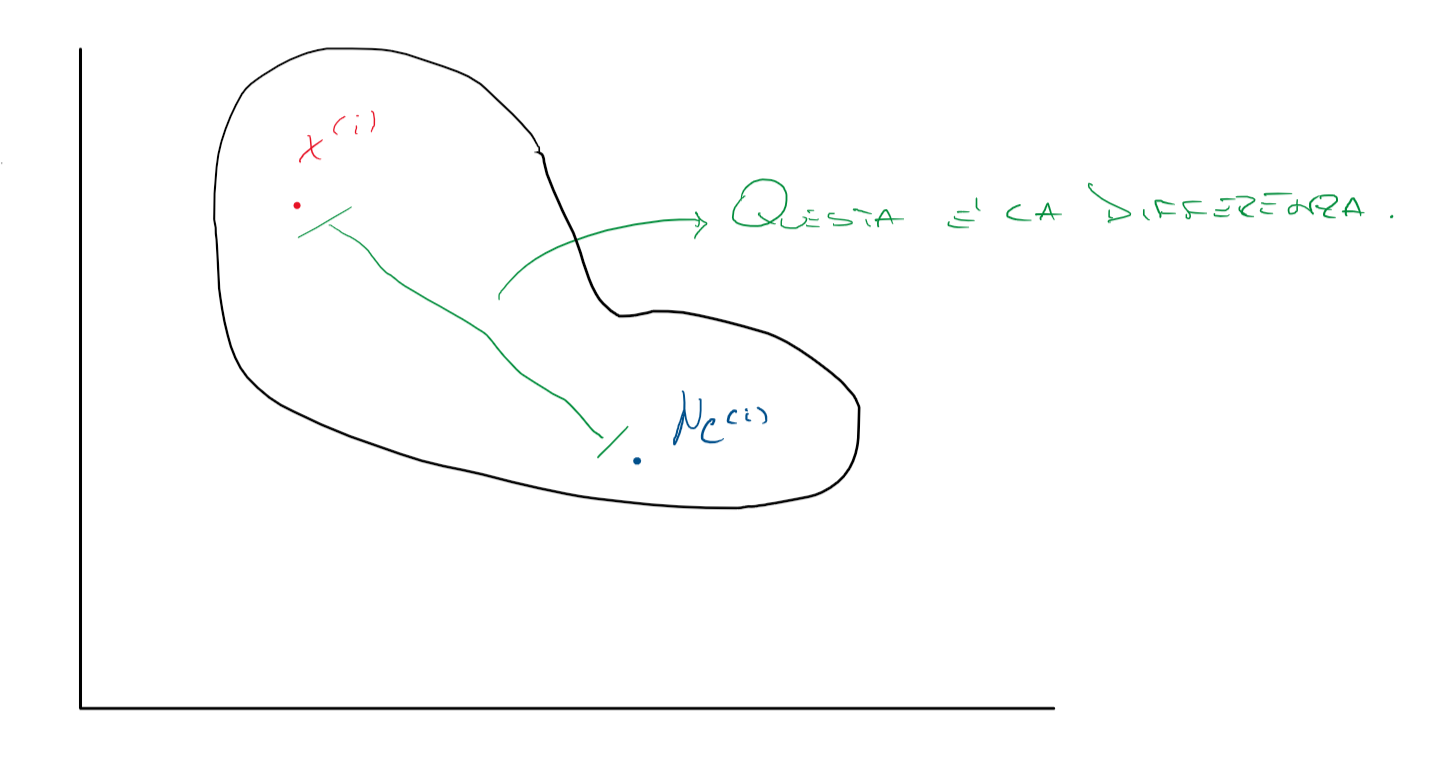
\includegraphics[width=0.7\textwidth]{img/kmeans6.PNG}
\end{figure}
\end{nota}
Dalla funzione di costo notiamo alcune particolarità nell'algoritmo:
 \begin{figure}[H]
    \centering
    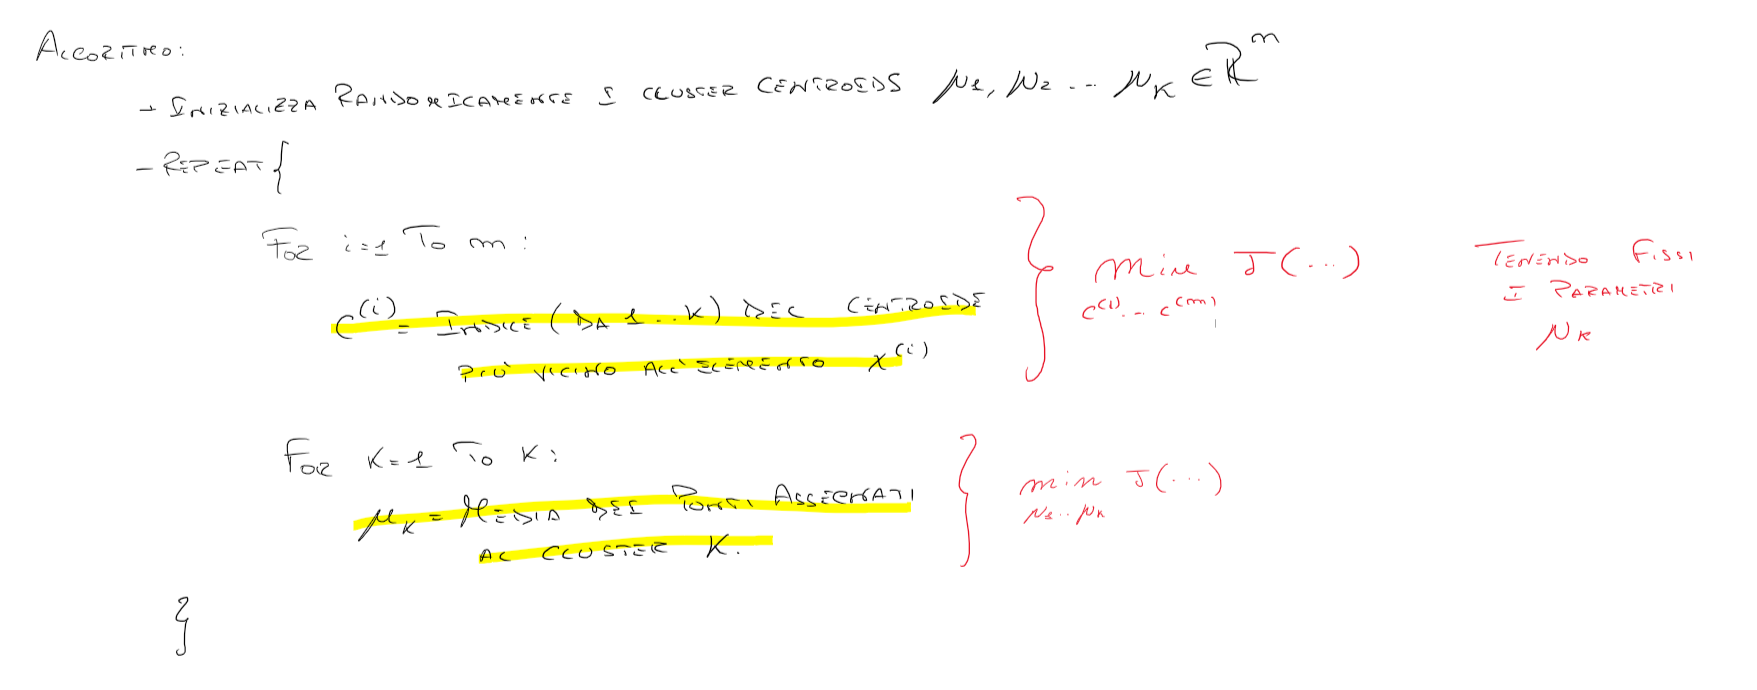
\includegraphics[width=1\textwidth]{img/kmeans14.PNG}
\end{figure}
\subsection{Inizializzazione randomica dei centroidi}
Si è dimostrato che grossolani valori iniziali corrompano l'intero processo. Quindi, i cari lettori si staranno chiederanno: \textit{"Mario, quindi come facciamo a inizializzare i centroidi nel modo opportuno?"}.
\begin{enumerate}
    \item Prendiamo in considerazione $k$ elementi all'interno del dataset.
    \begin{nota}
    Non potendo avere più centroidi che elementi nel dataset, dovremo avere $k<m$.
    \end{nota}
     \begin{figure}[H]
    \centering
    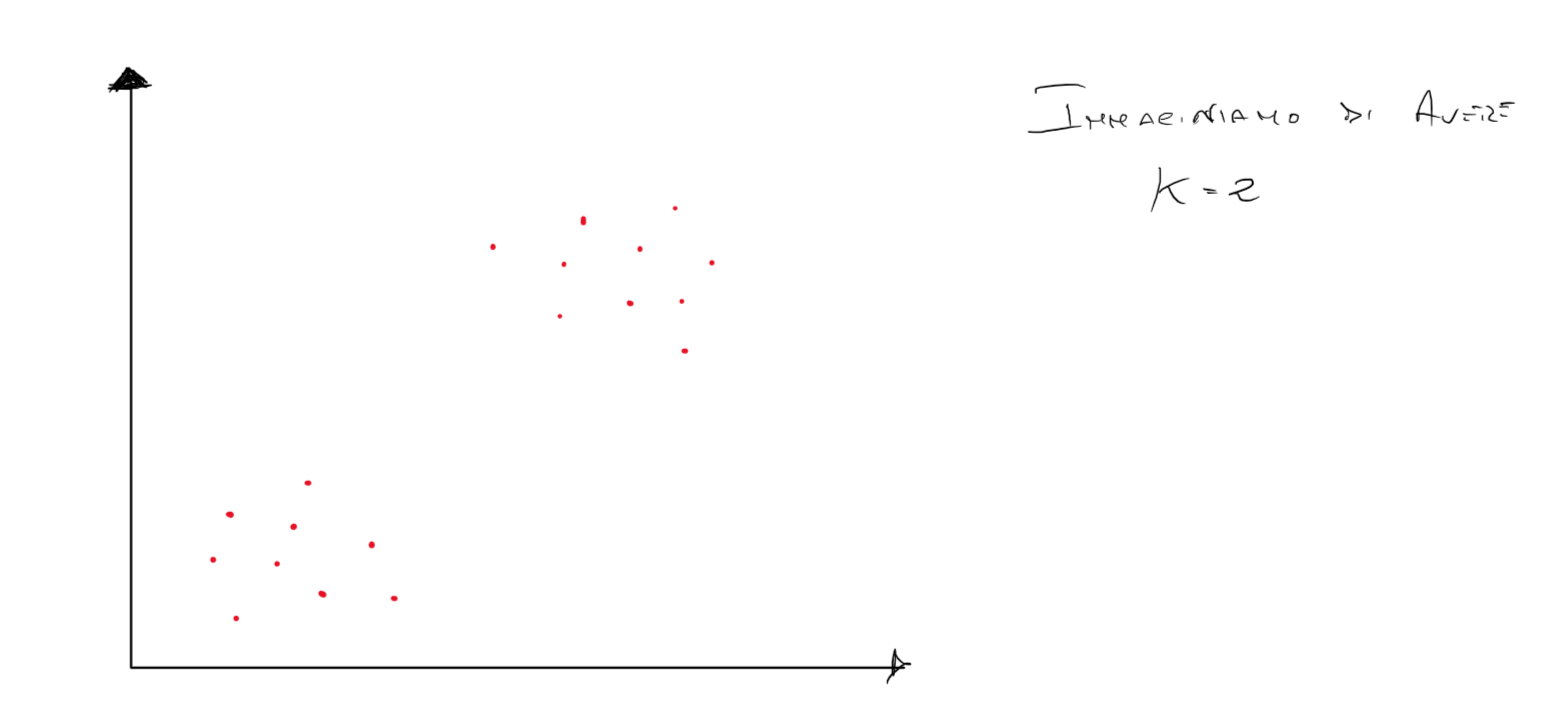
\includegraphics[width=0.7\textwidth]{img/kmeans7.PNG}
\end{figure}
    \item Impostiamo $\mu_1 \cdots \mu_k$ in base ai $k$ esempi presi in considerazione.
     \begin{figure}[H]
    \centering
    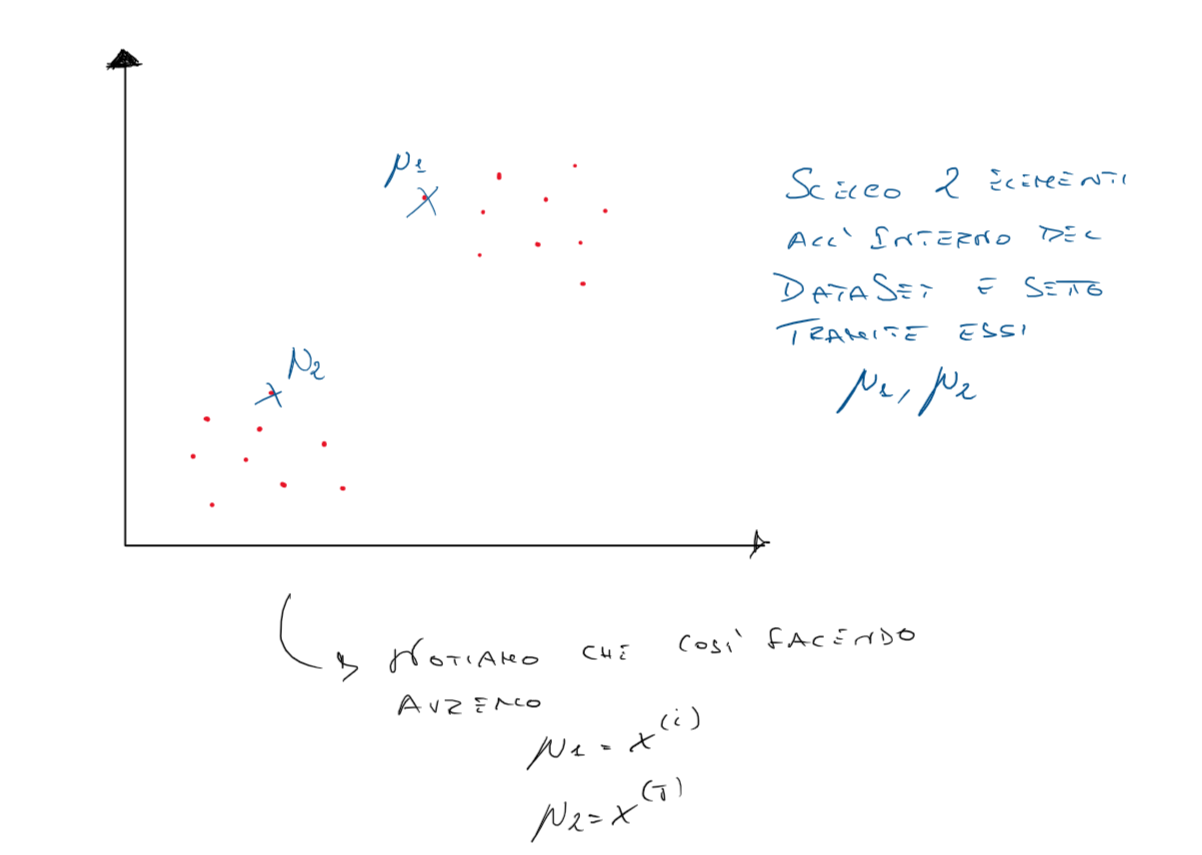
\includegraphics[width=0.7\textwidth]{img/kmeans8.PNG}
\end{figure}
\end{enumerate}
I cari lettori sempre molto attenti avranno notato un problema all'interno della procedura: \textit{"Se i centroidi venissero inizializzati in modo errato?"}.
     \begin{figure}[H]
    \centering
    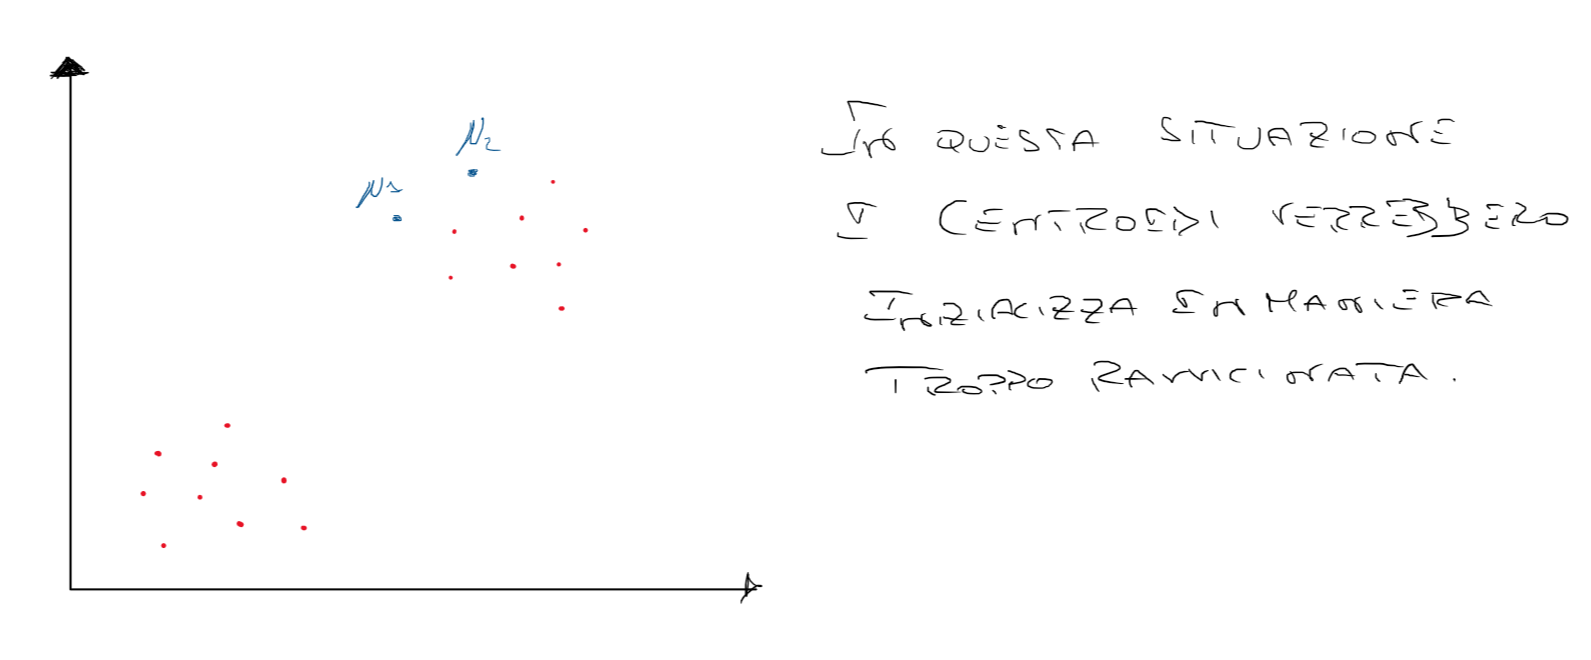
\includegraphics[width=1\textwidth]{img/kmeans9.PNG}
\end{figure}
     \begin{figure}[H]
    \centering
    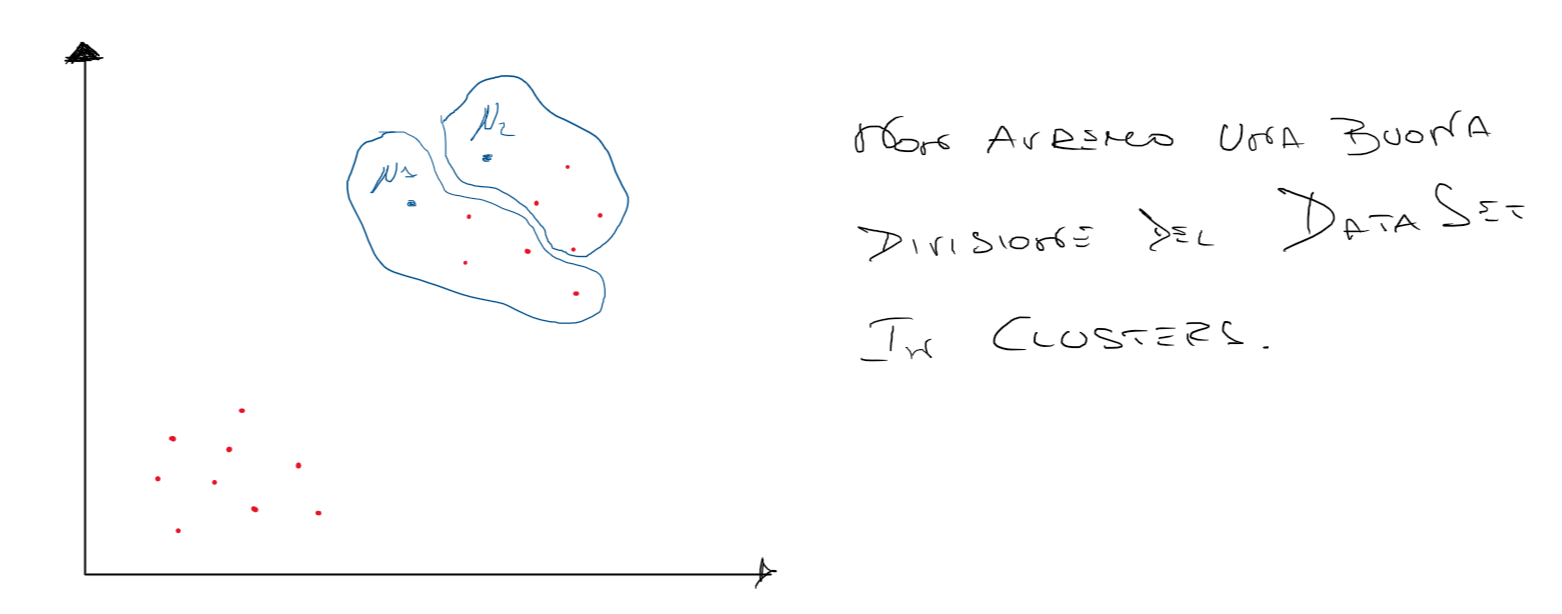
\includegraphics[width=1\textwidth]{img/kmeans10.PNG}
\end{figure}
Una possibile soluzione al problema è quella di eseguire l'inizializzazione e l'algoritmo per un certo numero di volte.
     \begin{figure}[H]
    \centering
    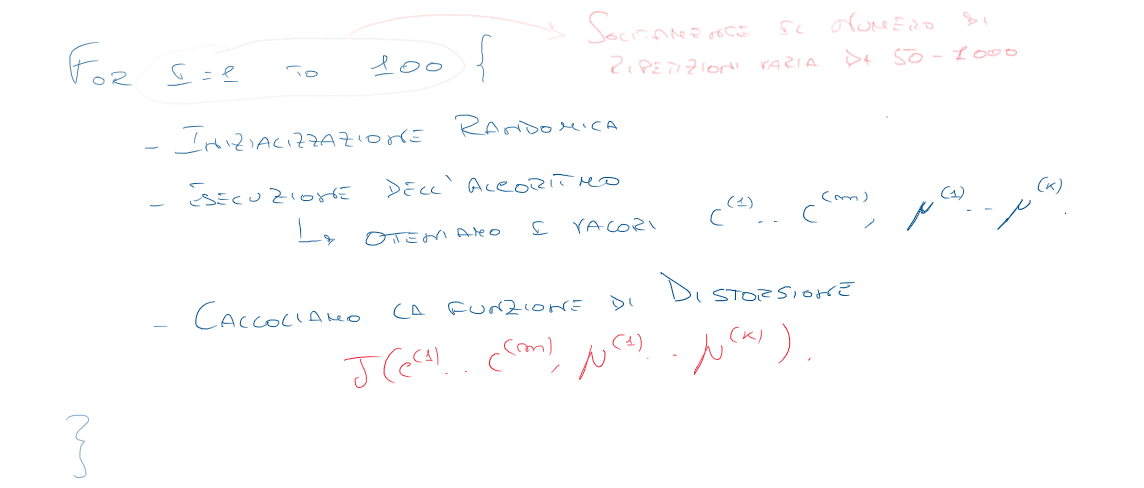
\includegraphics[width=1\textwidth]{img/kmeans15.PNG}
\end{figure}
Dopo un certo numero di iterazioni avremo diversi modi per classificare i dati in clusters. L'idea è quella di scegliere la soluzione \textbf{la cui funzione di costo è minore}. Il numero di iterazioni varia molto in relazione al parametro $k$:
\begin{itemize}
    \item Se $k \approx 10$ allora il numero di iterazioni sarà minore poiché il numero di cluster da analizzare è minore.
    \item Se $k >> 10$ avviene l'inverso.
\end{itemize}
\subsection{La scelta del parametro $K$}
Non sapendo a priori il numero di $K$ posso ottenere scarsi risultati magari non
avendo abbastanza centroidi. Adattarsi a un numero
``erato'' di centroidi può portare a risultati ``sporchi''. La scelta migliore per trovare il numero di clusters ottimali ricade \textbf{sempre} nell'analizzare per bene un dataset prima di agire. Difatti potrebbe risultare ambiguo far eseguire tale procedura ad un algoritmo.
     \begin{figure}[H]
    \centering
    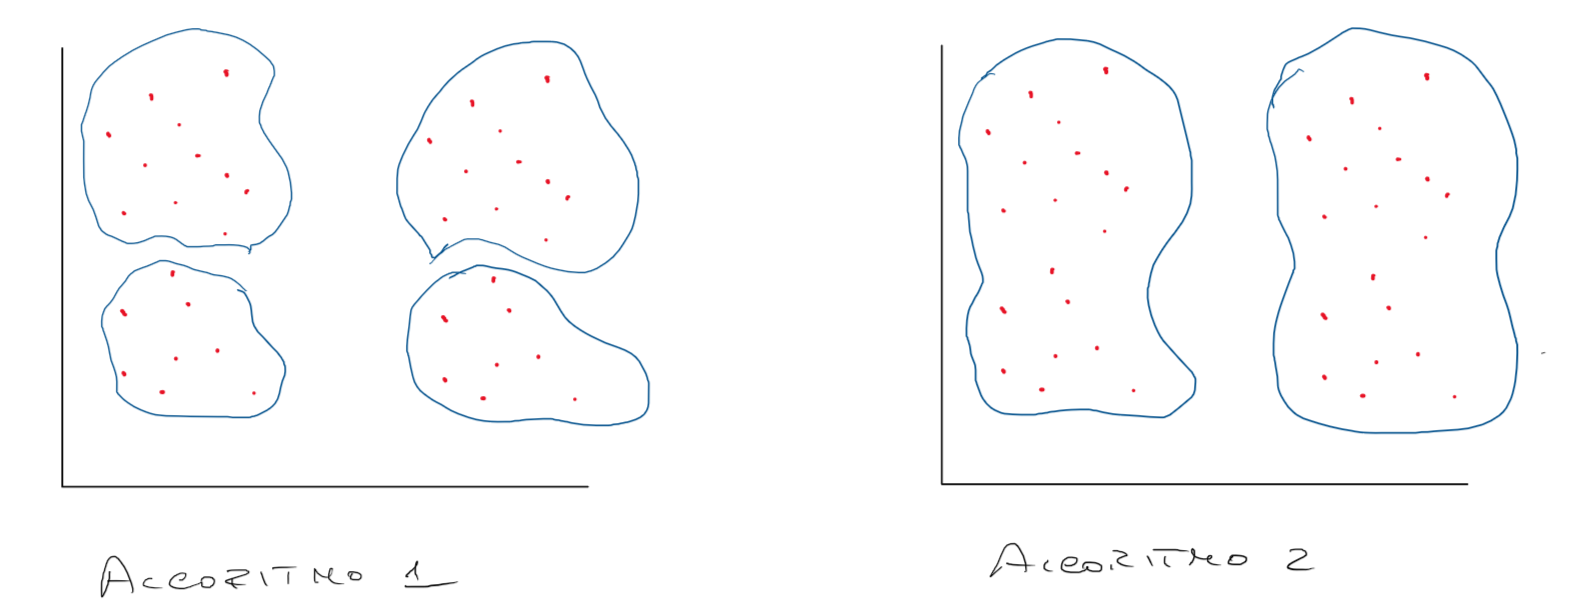
\includegraphics[width=1\textwidth]{img/kmeans11.PNG}
\end{figure}
Esistono però metodi più o meno efficaci per eseguire automaticamente tale procedura.
\subsubsection{Elbow Method}
\begin{definizione}(Elbow Method)
  From Wikipedia: Nell'analisi dei cluster, il metodo gomito è un metodo euristico utilizzato per determinare il numero di cluster in un set di dati. Il metodo consiste nel tracciare la variazione spiegata in funzione del numero di cluster e selezionare il gomito della curva come numero di cluster da utilizzare.
\end{definizione}
\begin{figure}[!htb]
   \begin{minipage}{0.48\textwidth}
     \centering
     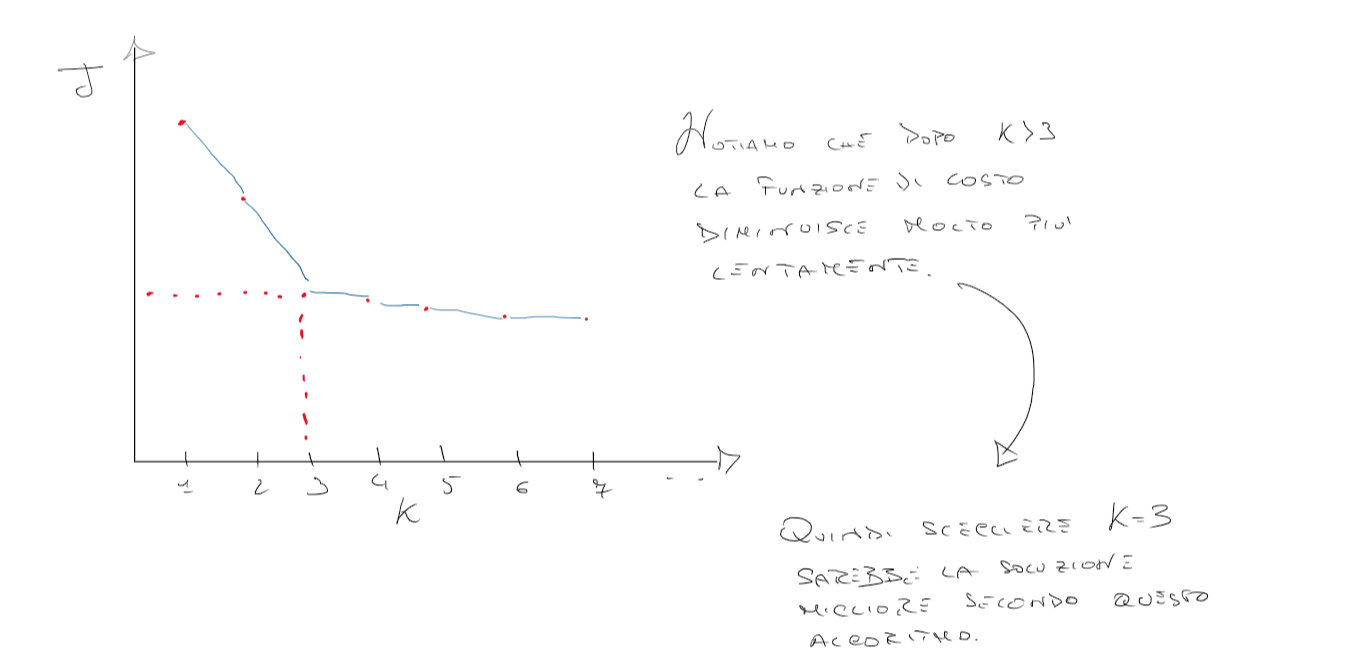
\includegraphics[width=1\linewidth]{img/kmeans12.PNG}
   \end{minipage}\hfill
   \begin{minipage}{0.48\textwidth}
     \centering
     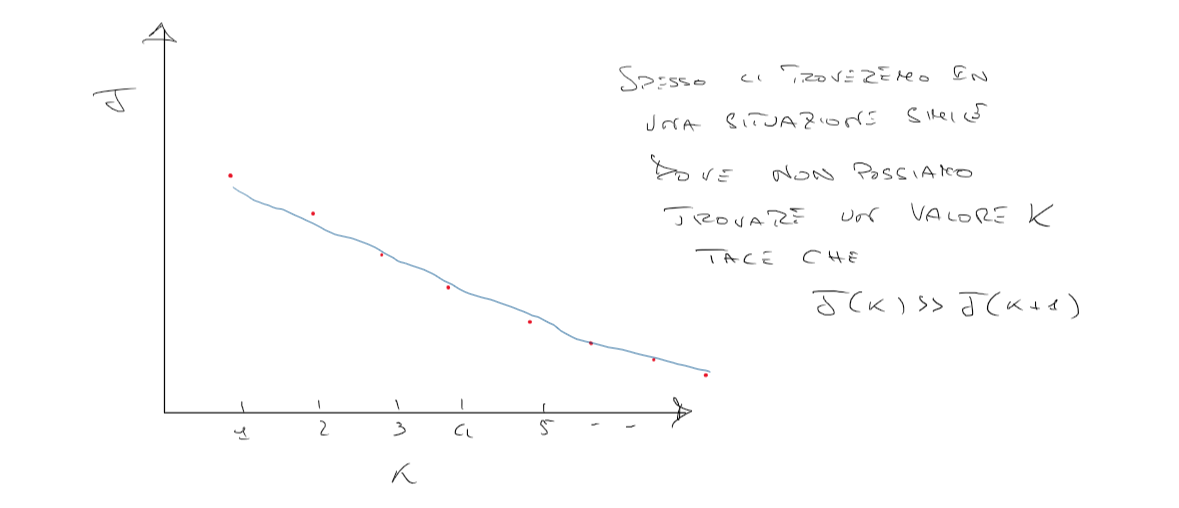
\includegraphics[width=1\linewidth]{img/kmeans13.PNG}
   \end{minipage}
\end{figure}
\subsection{Silhouette}
Per misurare le prestazioni di clustering bisogna capire come classificare i
risultati. Si usa la \textbf{misura di silhouette} per capire se un clustering è
migliore di un altro. Tale misura si basa sempre sul concetto di distanza. Si
ha una tecnica di misura, supponendo che ogni cluster abbia almeno due
elementi, avendo tecniche diverse qualora si abbia cardinalità 1, avendo la
distanza tra due elementi $d(i, j)$ e due concetti:
\begin{enumerate}
  \item \textbf{distanza media ``intra-cluster''}, ovvero dentro i cluster
  \[a(i)=\frac{1}{|C_i|-1}\sum_{j\in C_i, i\neq j}d(i, j)\]
  è buono se il valore è basso
  \item \textbf{distanza media ``inter-cluster''}, ovvero tra cluster:
  \[b(i)=\min_{k\neq i}\frac{1}{|C_k|}\sum_{j\in C_k}d(i, j)\]
  è buono se il valore è alto
\end{enumerate}
ottenendo quindi la \textbf{silhouette per il punto $i$}:
\[s(i)=\frac{b(i)-a(i)}{\max{a(i), b(i)}}\]

La qualità viene quindi visualizzata da un diagramma che studia la silhouette al
variare di $K$ per ogni valore di ogni attributo (mettendo per ogni attributo in
alto i valori più studiabili).\\
La media $s(i)$ su tutti i punti di un cluster è una misura di quanto siano
strettamente raggruppati tutti i punti del cluster. Pertanto, la media s (i) su
tutti i dati dell'intero set di dati è una misura di quanto adeguatamente i dati
sono stati raggruppati. Se ci sono troppi o troppo pochi cluster, come può
accadere quando una scelta sbagliata di $k$ viene utilizzata nell'algoritmo di
clustering, alcuni dei cluster mostreranno tipicamente
linee molto più strette rispetto al resto nel diagramma di silhouette. Quindi
grafici e media di silhouette 
possono essere utilizzati per determinare il numero ``naturale'' di cluster
all'interno di un set di dati. 
\subsection{Esempi}
\begin{esempio}
  Siano dati i seguenti 8 esempi:
  \begin{enumerate}
    \item $A1=(1, 10)$
    \item $A2=(2, 5)$
    \item $A3=(8, 4)$
    \item $A4=(5, 8)$
    \item $A5=(7, 5)$
    \item $A6=(6, 4)$
    \item $A7=(1, 2)$
    \item $A8=(4, 9)$
  \end{enumerate}
  $K=3$ e la distanza euclidea.\\
  Si supponga che all'inizio i tre centroidi (rispettivamente $seed1$, $seed2$ e
  $seed$3) siano $A1$, $A4$ e $A7$ avendo: 
  \begin{figure}[H]
    \centering
    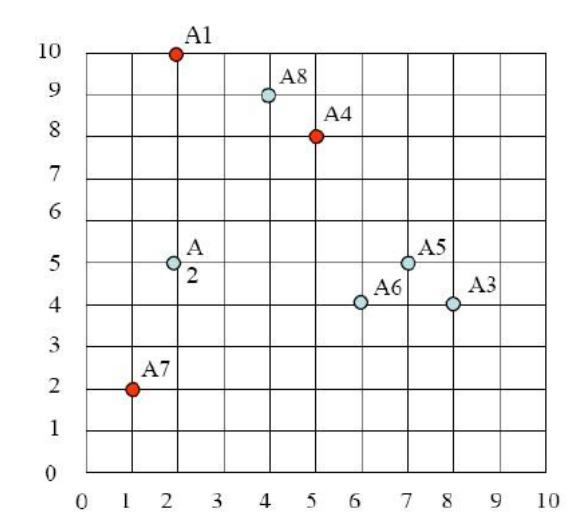
\includegraphics[scale = 0.4]{img/clue.jpg}
  \end{figure}
  \noindent
  e si esegua un'iterazione per ricalcolare i centroidi e i cluster associati.\\
  Usando la distanza euclidea procedo coi calcoli per generare i cluster,
  associando il cluster scegliendo il centroide che dista meno:
  \begin{itemize}
    \item per $A1$:
    \begin{itemize}
      \item $d(A1, seed1)=0$ essendo $A1$ il $seed1$ attuale
      \item $d(A1, seed2)=3.6$
      \item $d(A1, seed3)=8.06$
    \end{itemize}
    quindi $A1\in cluster1$
    \item per $A2$:
    \begin{itemize}
      \item $d(A2, seed1)=5$ 
      \item $d(A2, seed2)=4.24$
      \item $d(A2, seed3)=3.16$
    \end{itemize}
    quindi $A2\in cluster3$
    \item per $A3$:
    \begin{itemize}
      \item $d(A3, seed1)=6$ 
      \item $d(A3, seed2)=5$
      \item $d(A3, seed3)=7.28$
    \end{itemize}
    quindi $A3\in cluster2$
    \item per $A4$:
    \begin{itemize}
      \item $d(A4, seed1)=2.6$ 
      \item $d(A4, seed2)=0$ essendo $A4$ il $seed2$ attuale
      \item $d(A4, seed3)=7.21$
    \end{itemize}
    quindi $A4\in cluster2$
    \item per $A5$:
    \begin{itemize}
      \item $d(A5, seed1)=7.07$ 
      \item $d(A5, seed2)=3.6$
      \item $d(A5, seed3)=6.7$
    \end{itemize}
    quindi $A5\in cluster2$
    \item per $A6$:
    \begin{itemize}
      \item $d(A6, seed1)=7.21$ 
      \item $d(A6, seed2)=4.12$
      \item $d(A6, seed3)=5.38$
    \end{itemize}
    quindi $A6\in cluster2$
    \item per $A7$:
    \begin{itemize}
      \item $d(A7, seed1)=8.06$ 
      \item $d(A7, seed2)=7.21$ 
      \item $d(A7, seed3)=0$ essendo $A7$ il $seed3$ attuale
    \end{itemize}
    quindi $A7\in cluster3$
    \item per $A8$:
    \begin{itemize}
      \item $d(A8, seed1)=5$ 
      \item $d(A8, seed2)=2$
      \item $d(A8, seed3)=7.6$
    \end{itemize}
    quindi $A8\in cluster2$
  \end{itemize}
  Quindi nei nuovi cluster si ha:
  \begin{itemize}
    \item $cluster1=\{A1\}$
    \item $cluster2=\{A3, A4, A5, A6, A8\}$
    \item $cluster3=\{A2, A7\}$
  \end{itemize}
  Visualmente:
  \begin{figure}[H]
    \centering
    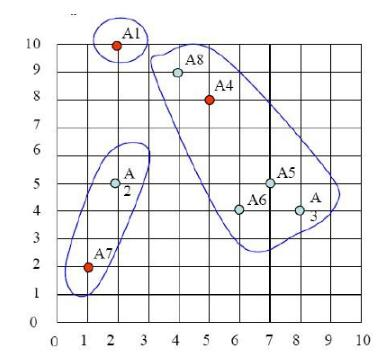
\includegraphics[scale = 0.4]{img/clue2.jpg}
  \end{figure}
  Posso fare le medie dei punti di ogni cluster per calcolare i nuovi
  centroidi: 
  \begin{itemize}
    \item $seed1New=(2, 10)$
    \item $seed2New=\left(\frac{8+5+7+6+4}{5},\frac{4+8+5+4+9}{5}\right)=(6, 6)$
    \item $seed3New=\left(\frac{2+1}{2},\frac{5+2}{2}\right)=(1.5, 3.5)$
  \end{itemize}
  Ovvero, segnando con una $x$ rossa i nuovi centroidi:
  \begin{figure}[H]
    \centering
    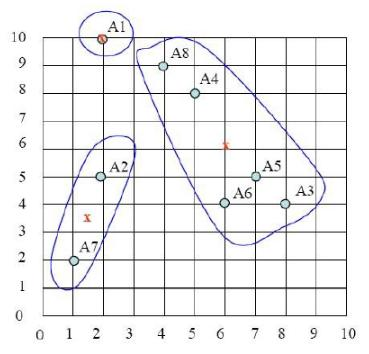
\includegraphics[scale = 0.4]{img/clue3.jpg}
  \end{figure}
  Avendo una sola epoca da calcolare mi fermo.
\end{esempio}
\chapter{Reinforcement learning}
\textit{Brevissima introduzione a caso}.\\
Questi metodi sono usati spesso in ambienti in cui serve trainare una macchina
magari per giocare a un gioco.\\
Si inserisce una maggiore ``distanza'' tra l'errore di prestazione del sistema e
la modalità di affinamento del comportamento. In questo tipo di apprendimento
l'errore è rappresentato come premio/punizione per il comportamento, non
vedendolo più come ``distanza'' per come era intesa in concept learning, SVM,
reti etc$\ldots$.\\
Quindi, nell'esempio di un gioco, si ha un ambiente con delle regole e dei
punteggi e questi vengono usati per il training, modificando il comportamento in
base ai punti, modificando le policy del comportamento. L'algoritmo che deve
cambiare le azioni dell'\textbf{agente} in base alle indicazioni dell'ambiente è
il fulcro del reinforcement learning. La definizione di tale algoritmo è quindi
ad hoc sul sistema in analisi e avere più informazioni implica una migliore
evoluzione. La variante più grossa è capire cosa si ha sbagliato in base ai
punti ottenuti.  \\
\textbf{Non si vede altro in merito.}
\chapter{Deep learning}
\textit{Brevissima introduzione, nelle slide c'è un approfondimento. L'argomento
comunque pare non essere nel programma d'esame (il prof l'ha detto due
volte)}.\\ 
Ad oggi la fama dei sistemi di apprendimento è associata al \textbf{deep
  learning}.\\
Dalle reti neurali si passa a reti multi-layer ``complete'', con algoritmi di
discesa del gradiente, funzioni di attivazioni, strumenti di regolarizzazione,
dati (tanti) e calcoli (tanti). Si hanno quindi sia aspetti qualitativi (come
l'uso di strumenti di regolarizzazione) che quantitativi (dati e calcoli).\\
Bisogna quindi studiare algoritmi di learning anche in queste ``nuove reti'',
per esempio appunto le \textbf{deep neural net}. Potrei avere anche reti con
cicli tra le sinapsi, ricorrenze, salvataggio in memoria, studi temporali
etc$\ldots$, \textbf{convultional neural net} e \textbf{recurrent neural net}
etc$\ldots$ (per uno schema vedere figura \ref{fig:neu}). Spesso tali reti sono
usate nel riconoscimento d'immagini, soprattutto le \textit{convultional
  neural net} (anche il passaggio da immagine a feature, prima manuale, è
stato integrato nelle reti). Si ha quindi un arricchimento di quanto studiato
fin'ora.\\
\begin{figure}
  \centering
  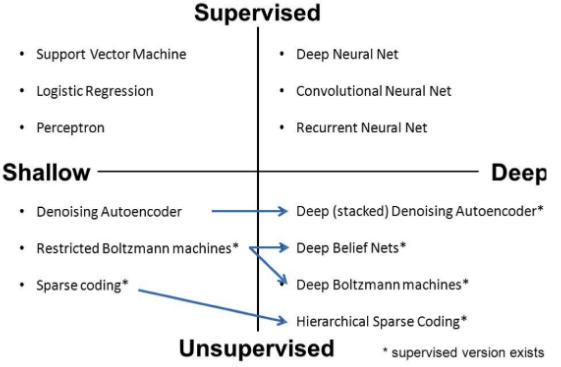
\includegraphics[scale = 0.6]{img/neu.jpg}
  \caption{Tassonometria delle reti neurali}
  \label{fig:neu}
\end{figure}
Una rete tradizionale, magari con due livelli (uno d'input e uno nascosto), e
lo applichiamo a un esempio base d'immagine: riconoscere una matrice di
numeri scritti a mano, detto \textbf{MNIST}. Si hanno 60000 immagini (di 784
pixel l'una, $28\times28$) di train e 10000 di test. Per lo studio si
appiattisce la matrice di pixel in un array. Usando una rete come appena
descritta, con tutto quanto, ha prestazioni di gran lunga superiore a quelle
classiche. Si ha uno studio approfondito delle varie funzioni di
attivazione. Tradizionalmente serviva una funzione derivabile mentre si
introducono funzioni non derivabili in qualche punto, modificando la discesa del
gradiente per funzionare anche in questo caso.\\
Lo schema base delle reti di questo tipo prevede l'arricchimento con molti
layer, completamente connessi tra loro (avendo tutte le possibili connessioni
tra loro), aumentando la complessità computazionale. Si ha inoltre un parametro
$\alpha$ che riduce i pesi verso lo zero, controllando la regolarizzazione.\\
Un'altra struttura usata è l'\textbf{autoencoder} che non è ``deep'' ma moderna
come gli strumenti ``deep'' ed è usata per l'apprendimento non
supervisionato. In questo caso si hanno uno o più layer nascosti con una certa
funzione di attivazione ma con meno neuroni delle feature in input. Non avendo
un'etichetta, non essendo supervisionato, addestro il sistema sul confronto tra
gli output (che quindi è di cardinalità pari al numero di feature in input) e
gli input, in modo ciclico. Come per le reti altero i pesi in base all'errore
calcolato (in questo caso direttamente tra input e output).\\
I pesi a fine addestramento possono anche dirmi quali connessioni sono diventate
``più forti''. Ogni layer nascosto è quindi una codifica del dato.
Questo approccio può essere usato per MNIST.\\
Il \textbf{deep learning} è quindi appunto l'apprendimento nei layer (molti). I
layer sono associati via via a concetti sempre più complicati. Mettendo insieme
le astrazioni via via più complesse si ottengono i risultati. Questo ``schema''
si è ``scoperto'' sperimentalmente, le varie feature vengono infatti definite
automaticamente, per aggiornamento progressivo dei pesi. \\
Negli anni si è passati anche a dataset più complessi di MNIST, magari come
CIFAR-100, per testare algoritmi di deep learning sempre più complessi.\\
In merito allo studio delle immagini si hanno anche le \textbf{convoluzioni} e
le \textbf{max pooling}. Le max pooling seleziona i segnali più
dominanti/``forti'' di un gruppo di neuroni in una certa regione, riducendo la
cardinalità dell'insieme dei segnali (è una sorta di estrazione delle
informazioni). Le convoluzioni, che nel cervello umano sono 
connessioni tra neuroni che evidenziano il campo visuale, invece, rappresentano
il fatto che pixel vicini in ingresso alimentano singole zone di neuroni nel
layer successivo (se ho vari input per un pixel nel layer successivo saranno
tutti reindirizzati a un singolo neurone, perlomeno a livello parziale). Non si
ha più un connessione completa tra i neuroni ma una più specifica (non tutti con
tutti ma singole ``zone'' con alcuni neuroni).\\
Con regolarizzazione, il \textbf{dropout}, si indica invece l'evitare
l'overfitting ``sfumando'' lo spazio/ipotesi appreso, migliorando l'astrazione
uccidendo neuroni in una certa quantità (si ha una probabilità di eliminazione
associata ad ogni neurone). L'eliminazione è fatta progressivamente
nell'apprendimento della rete. \\
Tutte queste nuove tecniche permettono prestazioni migliori di
classificazione.\\
\textbf{Su slide esempio reale di struttura di deep learning per CIFAR-100.}
\chapter{Misura delle performance}
\textbf{Questa parte è stata fatta per il laboratorio, è parecchio incompleta ed
è bene guardare anche le slide.}\\
Si studia quanto ci si può fidare di un modello e come classificare i risultati
di un modello, per capire se è migliore di un altro.
\section{Modelli supervisionati}
Partiamo dagli approcci supervisionati. \\
Uno egli indicatori è legato alla misurazione dell'errore sui dati di training e
testing (facendo training sul training e testing sempre sul training) ma questa
non è una buona misura ma si fa per capire se il modello ha buone performance su
dati ``ovvi'' ma questo non è garanzia di qualità, non studiando dati non
osservati in fase di training. Si rischiano overfitting/underfitting (nel primo
caso si impara molto bene sui dati di training ma quel modello appreso ha
performance basse e complessità computazionale alta su dati nuovi mentre nel
secondo caso il modello ha già performance basse e quindi risultati pessimi su
nuovi dati, anche se si ha minor complessità computazionale, avendo magari meno
parametri).
\begin{figure}
  \centering
  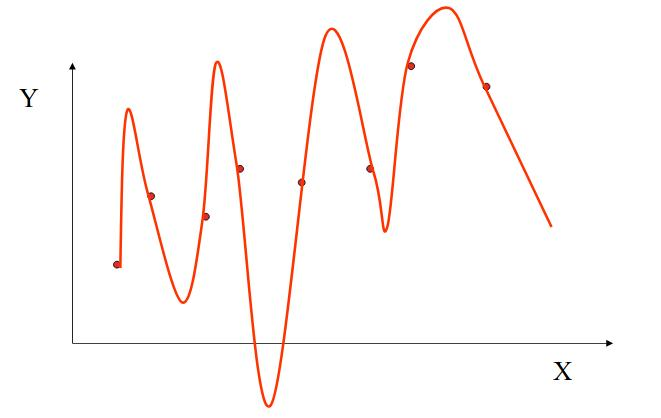
\includegraphics[scale = 0.3]{img/of.jpg}
  \caption{Esempio di modello in overfitting}
  \label{fig:over}
\end{figure}
Normalmente quindi si fa il testing su un testing set. Spesso è meglio avere un
modello meno preciso ma con complessità computazionale adeguata al dominio in
cui sto lavorando.
\begin{figure}
  \centering
  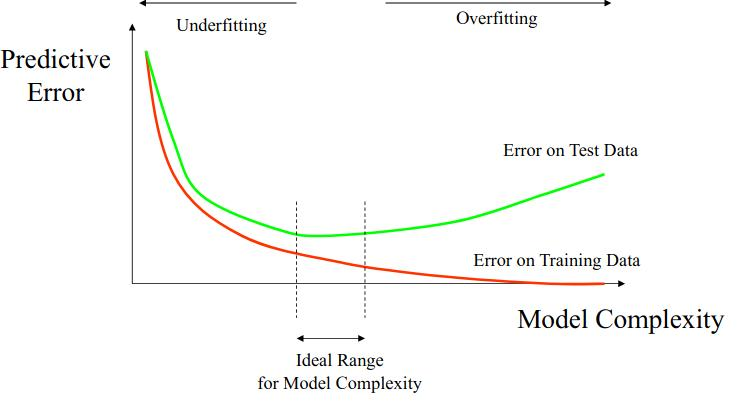
\includegraphics[scale = 0.5]{img/of2.jpg}
  \caption{Andamento di overfitting/underfitting sulla qualità del modello, con
    indicato il range ideale. Spesso sull'asse delle $x$ si ha il numero di
    iterazioni necessarie per capire quando terminarle per non andare in
    overfitting, come nel caso delle reti neurali}
  \label{fig:over2}
\end{figure}
Si hanno quindi varie misure di performance:
\begin{itemize}
  \item error rate e accuratezza
  \item true/false positive/negative
  \item precisione, recall, F-Measure
  \item curve ROC
  \item complessità temporale
\end{itemize}
Si hanno quindi:
\begin{itemize}
  \item successo, se le istanze sono predette correttamente
  \item errore, se le istanze non sono predette correttamente
\end{itemize}
Calcolando, per il primo punto:
\begin{itemize}
  \item l'error rate come percentuale di errori commessi sull'intera serie di
  istanze 
  \item accuratezza come proporzione d'istanze classificate correttamente
  sull'intero set d'istanze 
\end{itemize}
Passiamo al secondo punto.\\
Normalmente si munta a minimizzare falsi positivi/negativi anche se tutte e 4 le
entry della matrice di confusione andrebbero ottimizzate (con le entry che
possono avere costi 
diversi a seconda del dominio, si pensi alle diagnosi mediche dove i falsi
negativi sono più gravi dei falsi positivi).\\
In un problema multiclasse ho su righe e colonne le classi reali e le classi
predette, rispettivamente, non avendo più chiari i veri/falsi positivi/negativi,
che comunque possono essere ricavati per ogni classe.\\
\begin{definizione}
  Definiamo (in pratica per il caso binario):\\
  \textbf{accuratezza}:
  \[\frac{TP+TN}{TP+TN+FP+FN}\]
  (che nel caso multiclasse è la somma dei valori sulla diagonale principale
  diviso la somma del resto)\\
  \textbf{precisione}:
  \[\frac{TP}{TP+FP}\]
  \textbf{recall}:
  \[\frac{TP}{TP+FN}\]
  \textbf{F-measure}:
  \[\frac{2\cdot precisione\cdot recall}{precisione+ recall}\]
  \textbf{Queste sono le tradizionali misure globali.}
\end{definizione}
Si costruiscono quindi le matrici di confusione a seconda del caso binario o
multiclasse. Ma per il caso multiclasse posso calcolare solo la precisione di
una singola classe, come anche per recall e F-measure.\\
Spesso quindi si lavora a livello di classe.
\begin{definizione}
  Si hanno, data una label $l$ nell'insieme delle etichette $L$:\\
  \textbf{precisione}:
  \[P(l)=\frac{\# \text {of instances correctly predicted as } 1}{\#\text {of
        instances predicted as } 1}\]
  \textbf{recall}:
  \[R(l)=\frac{\# \text {of instances correctly predicted as } 1}{\#\text {of
        instances of class } 1}\] 
  \textbf{F-measure} (ovvero tramite media armonica):
  \[F(l)=\frac{2 \cdot P(l) \cdot R(l)}{P(l)+R(l)}\]
  Potrei avere un parametro $\beta$ per dare più importanza a una certa classe.
\end{definizione}
Si hanno modi per aggregare le misure di performance per scoprire comportamenti
particolari. 
\begin{definizione}
  Data un'etichetta $l$ ho due tecniche di aggregazione:\\
  \textbf{Macro-average} di una misura di performance $Perf$:
  \[\text {Perf}\,^{*}=\frac{1}{|L|} \sum_{i=1}^{|L|} \text {Perf}(l)\]
  dicendo che tutte le classi sono ugualmente importanti e hanno tutte lo stesso
  peso.\\
  \noindent
  \textbf{Micro-average} dove ho una media pesata:
  \[\text {Perf}\,^{*}=\sum_{l=1}^{|L|} \frac{|class(l)|}{\#\text{of istances}}
    \text {Perf}(l)\] 
  Dando quindi più peso alle classi più ``corpose'' e predominanti.
\end{definizione}
Parliamo ora di curve \textbf{Receiver Operating Characteristic (\textit{ROC})},
che rappresentano delle curve che dimostrano la 
capacità discriminativa di un modello al variare di una certa soglia. Si
confrontano veri/falsi positivi al variare di una certa soglia (che varia la
variabile sperimentale). Variare la
soglia permette di avere decisioni diverse e permette di costruire la curva
ROC. In problemi con tante classi, soprattutto se alcune sotto dimensionate, si
rischia di non riconoscerle queste classi ma abbassando la soglia si può aiutare
il modello a riconoscerle. \textbf{Si ha una curva ROC per ogni classe} (con una
soglia unica però). L'uso delle curve ROC è comodo per fare tuning su modelli
indotti da dati molto sbilanciati. Si confrontano i vari modelli a seconda delle
singole classi studiando l'impatto della soglia. 
\begin{figure}
  \centering
  \includegraphics[scale = 0.5]{img/roc.jpg}
  \caption{Esempio di curva ROC per una certa classe. Se una curva, associata ad
    un certo metodo, domina tutte le altre allora quello è il metodo
    migliore. Se vale per ogni classe non si hanno più dubbi.}
  \label{fig:roc}
\end{figure}
Passiamo ora alla \textbf{learning curve}. Sono utili per studiare come evitare
l'overfitting, confrontando la cardinalità degli esempi con una miusra di
performance, come l'accuratezza. a un certo punto si arriva a un plateau e
quindi è inutile aumentare il numero di esempi (e la complessità computazionale)
se tanto non si hanno miglioramenti. Non solo, si aumenta anche la probabilità
di overfitting. 
\begin{figure}
  \centering
  \includegraphics[scale = 0.5]{img/lc.jpg}
  \caption{Esempio di learning curve.}
  \label{fig:roc}
\end{figure}
Normalmente abbiamo lavorato con train e test (divisi circa per $\frac{2}{3}$ e
$\frac{1}{3}$, rispettivamente, per poi trainare il modello sul training e
testare i risultati sul test) ma questa è una visione parziale.  \\
In generale più è grande il test set e più accurata la stima
dell'errore. D'altro canto più è grande il training set e meglio sarà fatta la
classificazione, al più di overfitting. Il test set non deve essere usato per il
training e per il tuning ma si usa il validation set per il tuning, che quindi è
un set aggiuntivo usato per ottimizzare i parametri (soglia, parametro di
complessità della SVM etc$\ldots$) quando il dataset è abbastanza grande da
permetterlo. Il validation è solitamente il $10\%$ del training set.\\
Se il dataset è piccolo magari la divisione appena detta non è rappresentativa
ma si usano tecniche di \textbf{repeated holdout}, in cui si divide più volte
usando di volta i dati nei vari set. Si usa la \textbf{cross-validation} e la
\textbf{k-fold-cross-validation} dove si hanno due step:
\begin{enumerate}
  \item i dati vengono suddivisi in $k$ sottoinsieme di uguale dimensione 
  \item ogni sottoinsieme a sua volta viene utilizzato per il test e il resto
  per l'addestramento 
\end{enumerate}
pesso i sottoinsiemi vengono stratificati prima che venga eseguita la cross
validation e viene calcolata la media delle stime di errore per fornire una 
stima complessiva dell'errore.\\
Per costruire una matrice di confusione su una time-fold-convalidation
costruisco per ogni iterazione di folding la matrice di confusione dello
specifico test set e alla fine le si somma per ottenere la matrice finale.\\
Una variante è la \textbf{stratified ten-fold cross-validation} in quanto
esperimenti approfonditi hanno dimostrato che questa è la scelta migliore per
ottenere una stima accurata (usare 10 fold) e avendo che la distribuzione delle
istanze selezionate, rispetto alla classe da prevedere in ogni volta, è simile
alla distribuzione originale del set di dati (per lo stratified). La
stratificazione riduce la stima  
della varianza ma è ancora meglio ripetere tale stratificazione dieci volte.\\
Si hanno altre tecniche definite di \textbf{bootstrap} che utilizzano il
campionamento con rimpiazzo dal training set, avendo che la stessa istanza può
finire puiù volte nello stesso ``esperimento'' di time fold cross validation. Le
istanze del dataset originale che non compaiono nel nuoo training set vengono
usate come test. \textbf{Su slide 0.632 bootstrap, una tecnica empiricamente
  efficiente ma poco usata per la distorsione dei risultati a casua del suo
  pessimismo intrinseco}.\\
Una tecnica alternativa è \textbf{leave-one-out} che perfeziona il bootstrap. In
questa tecnica si ha una $k$ fold validation con $k$ pari al numero delle
istanze. Un'istanza sola viene lasciata per il test e tuutte le altre per il
training, cambiando ad ogni iterazione quella di testing fino ad esaurimento. È
computazionalmente pesante ($n$ fold per $n$ istanze) ma fa il miglior uso dei
dati. \\
Da un punto di vista metodologico vediamo ora come misurare la robustezza di un
modello, anche rispetto a un altro modello. Si misurano quindi gli
\textbf{intervalli di confidenza} per un certo livello di confidenza. Tra
modelli si confrontano quindi gli intervalli di confidenza, preferendo quello
con intervallo più stretto (per l'intervallo esempi con t-student). Oltre alle
misure già elencate precedentemente si 
usa anche l'entropia (\textbf{esempio su slide}).\\
Un secondo elemento per preferire un modello a un altro (dicendo che
``out-performa'' l'altro) è usare i \textbf{test di significatività}. Per farlo
si usa il \textbf{test della t-student} e se i due modelli stanno lavorando
sulla stessa configurazione di fold allora posso usare il \textbf{paired t-test}
confrontando direttamente le predizioni, non avendo variabilità sperimentale tra
i due risultati. \textbf{Sulle slide eventuali formule per il calcolo riprese
  dalle basi di statistica}.\\
Quindi:
\begin{itemize}
  \item si fissa il livello di significatività desiderato (normalmente $95\%$)
  \item si divide per due avendo un test a due cose
  \item si cerca il valore di $z$
  \item se $t\leq -z$ o $t\geq z$ la differenza è significativa
\end{itemize}
Potrebbe capitare che un t-test paired non sia effettuabile, anche solo se nel
mezzo del lancio dei modelli si ha un fattore di randomicità o avendo una $k$
diversa di fold convalidation.\\
In generale:
\begin{itemize}
  \item non basarsi solo sui numeri per le prestazioni
  \item guardare bene l'output del modello
  \item non trascurare la complessità del modello
\end{itemize}
\section{Modelli non supervisionati}
Si hanno diverse tecniche per studiare la bontà del clustering tra cui:
\begin{itemize}
  \item clustering tendency
  \item clustering quality
\end{itemize}
Per la \textbf{cluster tendency} ci dice che bisogna verificare se i dati hanno
una certa tendenza e che non siano punti distribuiti uniformemente nello
spazio. Per studiare la cosa all'aumentare delle dimensioni si usano:
\begin{itemize}
  \item \textbf{Hopkin statistic} che studia la probabilità che il dataset sia
  generato con distribuzione uniforme, campionando $N$ punti e calcolando la
  distanza da ogni punto rispetto al punto più vicino. Si genera quindi un
  dataset simulato, campionando da una distribuzione uniforme e infine si
  calcola con:
  \[H=\frac{\sum_{i=1}^{n} y_{i}}{\sum_{i=1}^{n} x_{i}+\sum_{i=1}^{n} y_{i}}\]
  $H$ (hopkin statistic) oltre $0.75$ indica clustering tendency al $90\%$ di
  livello di confidenza
  \item  \textbf{VAT algorithm} dove si calcola la matrice di dissimilarità e si
  mettono vicini gli elementi simili, creando una matrice a blocchi riducendo il
  problema ad due dimensioni, facilmente visualizzabile
\end{itemize}
In merito al \textbf{clustering quality} posso misurare misure interne
(silhouette, somma dei quadrati etc$\ldots$) ma anche esterne (precisione,
recall etc$\ldots$), qualora si abbia a che fare con anche le classi ottenute
dal cluster. Posso quindi fare t-test paired o unpaired a seconda della
situazione. %7

%----------------------------------------------------------------------------------------
%	BIBLIOGRAPHY
%----------------------------------------------------------------------------------------
\printbibliography
%----------------------------------------------------------------------------------------
\end{document} 

% LocalWords:  Machine Learning machine learning dataset fit overfitting sse 
% LocalWords:  Concept concept experience learner rewards inductive validation
% LocalWords:  find Find findS version List biased Hypothesis unbiased bias yes
% LocalWords:  bias prover information gain slide level sibling distance wind
% LocalWords:  weak outlook sunny humidity high normal overcast rain branch IG
% LocalWords:  primis True backtracking greedy overfit split Description Length
% LocalWords:  cloudy rainy warm cold sky temp humid forecast same change Venn
% LocalWords:  darkgreen list then example label dell nell refractory Hebb pre
% LocalWords:  McCulloch Pitts sigmoide Percettrone percettroni iperpiano error
% LocalWords:  function Papert Minsky perceptron Recall feedforward layer Unit
% LocalWords:  Linear Treshold LTU soddisfacibilità replace percettrone ALVINN
% LocalWords:  retropropagazione nodes branches leef outcome pdf red Shannon VC
% LocalWords:  Support Vector Machines SVM Machines Vector Support LocalWords
% LocalWords:  iperpiani Cervonenkis Vapnik support vector kernel trick Bayes
% LocalWords:  riscalato Bayesano clustering Lagrange feature
